\documentclass[11pt,twoside]{report}

\usepackage[utf8]{inputenc} % En premier 

\usepackage[T1]{fontenc} % Pour taper les lettre accentuées
\usepackage{graphicx}
\usepackage{lscape}
\usepackage{array, multirow, makecell}
\usepackage{geometry}
\usepackage{amsmath}
\usepackage{fancyhdr}
\usepackage{float}
\usepackage[dvipsnames]{xcolor}
\usepackage{eurosym}
\usepackage{colortbl}
\pagestyle{headings}
\renewcommand{\baselinestretch}{1.2}

\usepackage[french]{babel} % En avant dernier
\usepackage{hyperref} % En dernier
\hypersetup{         % parametrage des hyperliens
    colorlinks=true, % colorise les liens
    breaklinks=true, % permet les retours à la ligne pour les liens trop longs
    urlcolor= blue,  % couleur des hyperliens
    linkcolor= black, % couleur des liens internes aux documents (index, figures, tableaux, equations,...)
    citecolor= black % couleur des liens vers les references bibliographiques
    }

\title{Prédiction des consommations totales et réelles des bâtiments incluant le comportement des usagers}
\author{Quentin Darakdjian}

\parskip=5pt % Espace entre 2 paragraphes
\geometry{hmargin=2.5cm,vmargin=1.5cm} % Reglage grossier des marges

\begin{document}
\setcounter{tocdepth}{2} % Supprime les subsections de la table des matières
\tableofcontents
%\listoffigures
%\listoftables
%\chapter*{Nomenclature}

\begin{tabular}{l|l}
AIE & Avenir Investir Environnement \\
BE & Bureau d'Etude \\
BET & Bureau d'Etude Technique \\
CIFRE & Convention Industrielle de Formation par la REcherche \\
ECS & Eau Chaude Sanitaire \\
IAD & Intelligence Artificielle Distribuée\\
SMA & Système Multi-Agents\\
STD & Simulation Thermique Dynamique \\
\end{tabular}

\chapter*{Introduction générale}
\addcontentsline{toc}{chapter}{Introduction générale}

Cette introduction présente le contexte mondial, l'organisation et les enjeux de la thèse et enfin le plan de ce manuscrit.

----- Ajouter quelque part: IEA EBC Annex53(2013) has proven that, concerning the total energy use in buildings, the 3 majorcauses of energy performance gaps are:
1- Human factor - responsible for 80\% of performance gap
2- Climate factor - responsible for 15\% of performance gap
3- Building intrinsic factor -  responsible for 5\% of performance gap
----- This number are from the paper of Peter Op't Veld and Ad van der Aa, Stakeholder analysis and impact areas in relation to occupant behavior in buildings - Positioning Annex66 ----------

\section*{Contexte}

La crise économique des années 2010 touche l'ensemble de l'économie occidentale et s'accompagne de la dégradation de plusieurs fondamentaux sociaux et environnementaux de notre société. Cette situation nous oblige à repenser nos modèles de développement et en particulier à nous interroger sur l'avenir de l'énergie qui fonde le développement du monde que l'on connait. Comme le confirme à chaque rapport le GIEC \cite{GIEC-14}, abondante et bon marché depuis la seconde révolution industrielle, l'énergie fossile apparaît aujourd'hui et depuis les chocs pétroliers comme rare et de plus en plus chère dans un contexte où la menace du changement climatique se renforce. Accentué par l'évolution démographique, c'est dans ce contexte que le controversé essayiste et scientifique Rifkin \cite{Rifkin-12} promeut la troisième révolution industrielle et considère la transition vers des systèmes énergétiques décarbonés comme prioritaires. Néanmoins la démarche de transition énergétique (Energiewende) est à mettre au crédit de l'Allemagne de 1980 qui a été le précurseur mondial de l'application d'énergie renouvelable à l'échelle industrielle. En France et à la suite du Grenelle de l'Environnement, cette transition énergétique est partagée par la grande majorité des politiques, afin d'atteindre l'engagement national du facteur 4 \footnote{Le facteur 4 en France correspond à une réduction des émissions par quatre des GES entre 1990 et 2050} en 2050, tout en restant compétitif sur les marchés internationaux. L'association Negawatt \footnote{La sémantique du terme Négawatt quantifie une puissance en moins, c'est-à-dire une puissance économisée par un changement de technologie ou de comportement} a une forte notoriété pour la mise en œuvre de la transition énergétique de manière concrète et plus technique que le travail de Rifkin. L'accord de Paris de 2015 signé suite aux négociations de la COP21, est le dernier signe d'une volonté internationale de réduire le recours aux énergies fossiles et de réduire l'émission de gaz à effet de serre.

Cette contrainte de réduction des consommations d'énergie confronte nos sociétés à un défi d'une ampleur considérable. La consommation d'énergies fossiles à grande échelle est le socle qui a rendu possible le développement de nos sociétés modernes où aucune activité humaine n'échappe à la consommation d'énergie. En occident, le premier secteur consommateur d'énergie est le bâtiment, suivi des transports et de la production industrielle $Ref en fin de these$. Pour parvenir à l'objectif d'une société plus sobre en énergie, le secteur du bâtiment est donc une priorité tant son potentiel est jugé important et accessible à moyen terme. Compte tenu de l'état des technologies et par rapport aux transports, le bâtiment apparaît comme le domaine le plus mature pour la transition énergétique.

Cette amélioration continue des performances énergétiques des bâtiments neufs et anciens a été accompagnée par le développement d'outils de plus en plus performants et précis en termes de modélisation numérique. A l'inverse des premiers outils de calcul des déperditions statiques ne tenant même pas compte des apports solaires, les outils de simulations thermiques dynamiques actuels permettent d'intégrer l'ensemble des paramètres influençant le fonctionnement d'un bâtiment: climat, physique du bâtiment, équipements et usages. Alors que le niveau d'incertitude concernant les paramètres statiques liés à l'enveloppe, tels que les propriétés des matériaux ou le contrôle qualité de chantier, sont de plus en plus faibles, les incertitudes sur l'utilisation effective du bâtiment et le comportement des utilisateurs sont quant à elles très importantes. En résulte dans la pratique des écarts parfois considérables entre consommations théoriques et mesurées, d'autant plus élevés que la performance du bâtiment est grande. Au travers de l'amélioration des modèles des bâtiments, cette thèse doit permettre de mieux prendre en considération le comportement des usagers notamment par un état de l'art d'études sociologiques appliquées à l'énergétique du bâtiment et de développer un module de simulation pour le bureau d'études, AI Environnement, la structure d'accueil.

\section*{Force collective}

Comme nous venons de le voir, les pouvoirs publics ainsi que les associations non gouvernementales prennent des mesures pour panser les maux de notre monde. Certes, les moyens ne semblent pas toujours à la hauteur des enjeux, néanmoins les comportements individuels peuvent mener à des améliorations significatives. Cette philosophie a été imagée par l'histoire du mouvement Colibris de Pierre Rabhi: "Un jour, il y eut un immense incendie dans la forêt, seul un colibri déposa, goutte après goutte, de l'eau sur les arbres. "Tu crois que ce sont tes gouttes d'eau qui vont arrêter l'incendie?", se moquèrent les autres oiseaux. Et le colibri de répondre: "Seul, non, mais j'aurais fait ma part." Le projet de la tour Elithis de Dijon, se voulant être le premier bâtiment tertiaire à énergie positive, est un exemple d'application du mouvement Colibris. Lors de sa mise en service la tour ne consommait que 20 $kWh/m^2/an$, soit six fois moins qu'un bâtiment tertiaire standard, mais toujours 20 $kWh/m^2/an$ de trop pour véritablement atteindre l'objectif. Or, ce n'est pas un acharnement technologique qui a permis cela, mais l'accompagnement des employés vers des comportements en adéquation avec ce bâtiment et son environnement. % Mettre en référence Perrine Moulinié.

Colibris et les mouvements semblables sont des accélérateurs de transition, en s'appuyant sur la capacité de chacun à changer et à incarner ce changement dans des expériences concrètes et collectives. Cela encourage l'émergence et l'incarnation de nouveaux modèles de société fondés sur l'autonomie, l'écologie et l'humanisme.

\textit{"Les Colibris, ce sont tous ces individus qui inventent, expérimentent et coopèrent concrètement, pour bâtir des modèles de vie en commun, respectueux de la nature et de l'être humain."} P. Rabhi

\section*{Thèse en entreprise}

Le travail présenté dans ce manuscrit est le produit d'une thèse en contrat CIFRE (Convention Industrielle de Formation par la Recherche) c'est à dire co-financée par une entreprise, supervisée par un laboratoire et subventionnée par l'ANRT (Association Nationale de la Recherche et de la Technologie). Dans une démarche d'innovation et pour structurer ses activités de recherche et développement, AI Environnement, le bureau d'études techniques et Antoine Boulla, ingénieur d'étude et encadrant principal de la thèse, ont ressenti le besoin de mieux appréhender le comportement des usagers pour leurs études énergétiques. C'est dans ce contexte que la synergie avec l'Université de La Rochelle, par l'entremise de Christian Inard et Jean-Marc Ogier respectivement du LaSIE (Laboratoire des Sciences de l'Ingénieur pour l'Environnement) et L3I (Laboratoire Informatique, Image et Interaction) s'est établie. Afin de pouvoir confronter les résultats du modèle à des données réelles, Bassam Moujalled, membre du CEREMA \footnote{CEREMA: Centre d'Etudes et d'expertise sur les Risques, l'Environnement, la Mobilité et l'Aménagement \url{http://www.cerema.fr/}}, a été greffé dés le début du projet de thèse pour sa connaissance de la modélisation dynamique des bâtiments et sa proximité à des projets expérimentaux tests. Suite au départ d'Antoine Boulla d'AI Environnement en milieu de thèse, Sylvain Bille co-fondateur de l'entreprise en 2008 a repris l'encadrement. Enfin, à la suite d'un Master en Sciences et Techniques des Environnements Urbains à l'Ecole des Mines de Nantes, j'ai complété le groupe de travail afin de réaliser et articuler le projet.

La thèse en contrat CIFRE s'inscrit dans une logique de don contre-don où, par l'intermédiaire du doctorant, AI Environnement s'est lié à l'expérience de laboratoires de l'Université de La Rochelle tandis que les laboratoires ont recadré leurs activités de recherches aux besoins de la structure industrielle. Au milieu de cette synergie, le doctorant se retrouve parfois en situation inconfortable où il doit trouver l'équilibre entre les attentes des différentes parties tout étant l'acteur et le décideur principal du projet.

Au travers d'une telle thèse, le doctorant a un rôle d'interface entre le monde universitaire et le monde industriel. Bien que certains recruteurs voient encore la formation doctorale comme non professionnalisante, la CIFRE est vue d'une autre manière et tend à faire évoluer les mentalités. Les recruteurs industriels trouvent chez ces docteurs des compétences de pointe, d'une part de chercheur et d'autre part d'ingénieur familiarisé au milieu professionnel associé: double compétence valorisable.

\section*{Enjeux de la thèse et contribution}

C'est donc dans un contexte partagé entre le bureau d'études et les laboratoires, que cette thèse contribue à améliorer les résultats des projets thermiques et environnementaux. La recherche de hautes performances énergétiques et environnementales amène les bureaux d'études techniques à réaliser des STD (Simulations Thermiques Dynamiques) afin d'optimiser les constructions et rénovations en diminuant leurs consommations et en améliorant le confort des occupants. Le constat est que la prise en compte du comportement de ces derniers est actuellement le maillon faible de ce genre d'études. Face au manque d'informations concernant le comportement réel des usagers et leurs interactions avec le bâtiment, les thermiciens et énergeticiens sont contraints à en simplifier les hypothèses d'entrée. En effet, aujourd'hui ce comportement humain est grossièrement réduit à un taux d'occupation, une présence journalière répétitive via une approche très déterministe.

De nombreuses raisons ont été avancées pour expliquer la non-précision et la non-fiabilité des résultats des études de STD. Cependant, les résultats de l'Annexe 53 \cite{Annex-53-1}\footnote{Présentation et publications: \url{http://www.iea-ebc.org/index.php?id=141}}, \textit{Total Energy Use in Buildings: Analysis and Evaluation Methods}, projet de l'Agence Internationale de l'Energie (AIE), montrent que la principale cause d'incertitude provient de la mauvaise prise en compte du comportement des occupants. Dans la continuité à ce projet, l'Annexe 66, \textit{Definition and Simulation of Occupant Behavior in Buildings}\footnote{Site internet: \url{http://www.annex66.org/}} a été lancée avec des objectifs et des problématiques de recherche qui coïncident à ceux de la thèse, à savoir:
\begin{itemize}
\item Identification quantitative et classification du comportement des occupants sur les besoins énergétiques du bâtiment
\item Création d'une base de données sur les comportements des occupants au sein des modèles
\item Implémentation des modèles dans les outils de simulation énergétique des bâtiments
\item Évaluation des modèles de comportement développés par des études de cas
\end{itemize}
L'intérêt de cette Annexe et la période de travail (2014-2017) m'a donc amené à intégrer ce groupe de travail international et à participer aux différentes réunions (Nottingham, Berkley, Karlsruhe, Vienne). Des participations à ces types de regroupements font partie du travail des chercheurs, car elles permettent d'échanger et de mettre en commun les connaissances et avancées.

\section*{Plan du manuscrit}

Nous proposons une lecture du manuscrit qui peut être découpée en plusieurs parties. Le premier chapitre évoque la situation de la conception et de la construction des bâtiments en France. Le second chapitre traite de la différence de performance théorique et réelle...
\part{Etat de l'art}

\chapter{Conception et construction des bâtiments}

L'architecte est le chef d'orchestre d'un projet de construction. Il a une vision d'ensemble du projet et est le plus qualifié pour réaliser l'ensemble des missions, de l'étude de faisabilité du projet à la livraison en passant par la conception, la sélection des entreprises et la phase de chantier. Selon les exigences de la maîtrise d'ouvrage, l'architecte propose ses services de maître d'œuvre afin d'assurer une construction efficiente du bâtiment d'un point de vu technique mais aussi et surtout humain. 

La maîtrise d'œuvre, organisée autour de l'architecte, est composée selon les particularités des projets de bureaux d'études technique, d'économistes et d'autres partenaires. Les bureaux d'études thermique ont pour objectifs d'assister l'architecte dans les différentes phases du projet, afin d'une part d'attester la conformité du projet selon les normes en vigueur et d'autre part d'optimiser les performances thermiques et énergétiques des bâtiments.

Le travail de conception et de construction pour les spécialistes thermique et énergétique consiste pour beaucoup à représenter la réalité sous forme de modèles numériques. Ce travail de modélisation est ainsi présenté dans ce chapitre, ainsi que les calculs conventionnels, les certifications et les labels qui en découlent. Les Simulations Thermiques Dynamiques sont également au programme de ce chapitre, afin d'évoquer d'une part leurs intérêts, dont l'évaluation des performances futures et du confort des occupants et d'autre part de référencer certains outils.

\section{Modélisation numérique des bâtiments}

La modélisation énergétique est dans la phase de conception d'un bâtiment une étape d'optimisation indispensable. Basée sur des hypothèses simplificatrices elle vise à donner une image aussi proche que possible de la réalité afin de simuler l'exploitation du bâtiment. Cet outil d'aide à la conception fonctionne comme une plateforme d'essais virtuelle visant à étudier les options et à trouver une solution optimale. Ce travail porte généralement sur deux facteurs d'intérêts: le confort et la consommation énergétique.

Le bâtiment dans son ensemble est un objet complexe qui nécessite des simplifications pour sa simulation numérique. Une modélisation trop fine ne serait pas compatible avec les exigences des architectes et designers. Le niveau de modélisation doit alors être cohérence avec les objectifs du projet.

Le principe de modélisation est commun à l'ensemble des outils, et consiste à décomposer les volumes d'air en zones, séparés entre eux et de l'extérieur par des parois opaques et vitrées. Tout comme une paroi, une zone ne possède qu'un seul ensemble de variables d'état aux grandeurs homogènes (température, humidité, pression). Le couplage entre les zones se fait soit par conduction par l'intermédiaire des parois , soit par convection par l'intermédiaire des portes, fenêtres et infiltrations.

La simulation thermique dynamique permet d'obtenir les évolutions temporelles des variables de chaque zone. Le modèle du bâtiment est alors composé d'un ensemble d'équations de bilans enthalpiques et massiques qu'il est possible de résoudre en temps à condition de connaître les sollicitations thermiques environnantes.

\section{Calculs conventionnels}

Afin de créer un seuil minimum de performance énergétique des bâtiments, la législation a mis en place des réglementations thermiques évolutives. Ces règlementations imposent un calcul règlementaire indispensable pour obtenir un dépôt du permis de construire. La première réglementation fait suite au premier choc pétrolier de 1973 qui a déclenché une prise de conscience de la nécessité d'économiser l'énergie. Sa mise en place concerne les bâtiments neufs et date de 1974. Aujourd'hui et depuis le 1er janvier 2013, la Règlementation Thermique (RT) en vigueur est la RT 2012, elle précède la future Règlementation Bâtiment Responsable (RBR) 2020 et s'inscrit dans la continuité des RT 2005, 2000, 1988 et 1974 aux exigences croissantes. Depuis 2000, ces règlementations thermiques expriment des exigences sur les résultats en énergie primaire, alors que les RT antérieures imposaient des exigences de moyens, d'où leur absence sur la Figure \ref{fig:Evolution_des_performances_des_rt}. Impulsé par le Grenelle de l'Environnement les acteurs du bâtiment se préparent à une nouvelle évolution significative des performances à partir de 2020. Outre des améliorations techniques des matériaux, la RBR prendra également en considération les usages de l'électricité spécifique, l'énergie grise ainsi que de la mobilité qui est liée à la densité urbaine environnante. En effet, ces paramètres ne sont actuellement pas pris en considération dans la RT 2012 qui ne s'intéresse qu'à 5 postes de consommations (chauffage, climatisation, eau chaude sanitaire, éclairage et auxiliaires).

\begin{figure}
\centering
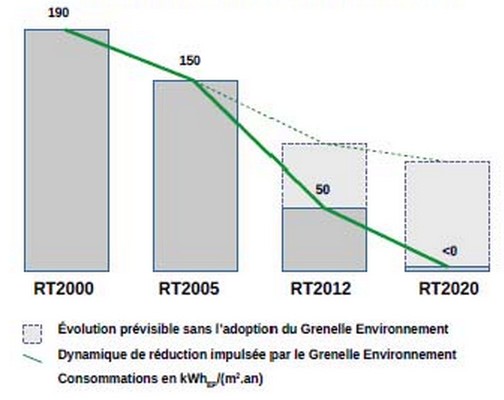
\includegraphics[scale=0.7]{Images/Evolution_des_performances_des_rt}
\caption{Évolution des exigences réglementaires de consommation énergétique des bâtiments neufs: une rupture opérée par le Grenelle Environnement. Source: Ministère de l'écologie, du développement durable et de l'énergie}
\label{fig:Evolution_des_performances_des_rt}
\end{figure}

La méthode de calcul actuelle (Th-BCE 2012), développée par le Centre Scientifique et Technique du Bâtiment (CSTB), n'a pas pour vocation de faire des calculs de consommations réelles mais de vérifier la normalité technique. Les paramètres du projet intervenant dans la méthode sont définis de façon conventionnelle, il s'agit notamment des données climatiques et relatives à l'usage des bâtiments. Plusieurs logiciels ont été développés en suivant le moteur de calcul Th-BCE 2012, les plus répandus en France sont Pleiades+COMFIE, Perrenoud, Clima-Win, DesignBuilder et CYPE.

\section{Certifications et labels}

Certains maîtres d'ouvrage éprouvent la volonté de construire des bâtiments plus performants que ce que les règlementations fixent. Les certifications et labels permettant de les catégoriser selon leurs modes de construction et leurs performances. Les certifications garantissent une construction ou une rénovation des bâtiments respectant de strictes exigences en termes de confort, santé, maîtrise des charges et environnementale. Les labels valorisent uniquement la performance énergétique des bâtiments, sans tenir compte des autres éléments. La diversité des certifications et des labels donnent la possibilité aux constructeurs puis aux futurs acquéreurs de choisir un logement répondant à leurs priorités et souhaits. Ainsi une certification couvre plus de champ qu'un label qui ne s'intéresse qu'à la dimension énergétique et qui ne peut être demandé qu'au sein d'une certification.

Plusieurs démarches ont été initiées dans les pays européens pour améliorer et codifier les démarches constructives. Les principes de l'éco-construction peuvent se décliner en France avec la certification de construction Haute Qualité Environnementale (HQE), définissant 14 cibles dans 4 domaines (éco-construction, eco-gestion, confort et santé) ou la certification \textit{BRE Environmental Assessment Method} BREAM, organisée autour de 10 catégories (gestion, bien-être et santé, énergie, transport, matériaux, eau, déchets, paysage et écologie, pollution et innovation). Les labels, tels qu'Effinergie ne peuvent être obtenus qu'après certification et intègrent donc également les principes de l'éco-construction. Les labels et certifications ne sont pas une spécificité française, en effet on peut retrouver Minergie en Suisse, Passivhaus en Allemagne, LEED en Amérique du Nord. En 2016, le label Bâtiment Bas CArbone (BBCA) a vu le jour afin d'évaluer l'empreinte carbone des opérations. Pour obtenir ce label un effort particulier doit être fait sur la construction elle-même. En effet, avec l'amélioration des performance énergétique des bâtiments en phase d'exploitation, une part très importante des émissions de gaz à effet de serre à lieu en phase de chantier. Ce label BBCA récompense alors les opérations qui utilisent des matériaux bio-sourcés et locaux ainsi que les chantiers qui recyclent leurs déchets.

Les intérêts de vouloir construire des bâtiments au delà des règlementations sont multiples. D'une part, cela apporte une visibilité au bâtiment car il mobilise des technologies nouvelles qui attisent la curiosité d'autres maîtres d'ouvrage et rendent donc le bâtiment désirable. Dans le domaine public les certifications peuvent être accompagnées de subventions ce qui permet de limiter d'éventuels sur-coûts. Aussi, par définition un bâtiment certifié ou labellisé est plus performant que la moyenne et réduira donc ses coûts d'exploitation pour un confort d'habitat à priori également amélioré. Un bâtiment certifié renvoie aussi à l'assurance que les meilleures pratiques de construction ont été intégrées au chantier. Alors que cette assurance de qualité, qui est une marque de reconnaissance, est sensée être recherchée par les maîtres d'ouvrage pour une future valorisation lors de la vente ou lors de la cession du bâtiment, il apparaît néanmoins que l'aspect économique inhibe bien souvent les bonnes volontés environnementales. La certification aborde les problèmes environnementaux dans leur globalité et permet aux promoteurs et concepteurs immobiliers d'amener de l'objectivité à la performance environnementale vis à vis de leurs clients.

La présentation des labels et certifications dans ce manuscrit se justifie par le fait que pour les attribuer il est nécessaire d'utiliser des logiciels qui quantifient les variables d'intérêts. La certification HQE impose par exemple des calculs d'éclairage, d'ensoleillement, d'Analyse de Cycle de Vie (ACV) et bien évidemment de Simulations Thermiques Dynamiques (STD).

\section{Simulations Thermiques Dynamiques}

Contrairement aux calculs conventionnels basés sur les règlementations thermiques, les STD offrent aux utilisateurs une liberté quasi totale sur le travail de modélisation avec pour objectif de s'approcher au maximum de la réalité. Avec l'accroissement des exigences de performances énergétiques et environnementales elle de plus en plus intégrée au processus de conception des bâtiments. Évaluer les besoins énergétiques et les puissances des systèmes d'un projet de construction requiert de disposer d'un certain nombre de données sur l'architecture, les conditions météorologiques et l'usage du bâtiment. La différence de résultats entre un calcul réglementaire et un calcul STD prévisionnel s'explique donc principalement par le fait que les que les scénarios réglementaires sont moyennés et éloignés de la réalité. Les variations s'expliquent principalement par le fait que le calcul réglementaire néglige ou sous estime certains postes de consommation d'énergie majeurs. Bien que la STD ait pour ambition de reproduire le comportement réel du bâtiment, elle ne peut être considérée comme une référence absolue. En effet, les hypothèses d'entrée du modèle et les modèles du calcul sont deux sources importantes d'erreurs de la simulation qu'il faut garder à l'esprit.

Un large panel de logiciels de STD est disponible pour simuler la performance énergétique et environnementale des bâtiments. Le \textit{Building Energy Software Tools} (BEST2016) \footnote{http://www.buildingenergysoftwaretools.com/} synthétise 45 d'entre eux et permet de les comparer entre eux. Les prochains paragraphes présentent des logiciels du domaine privé et de la recherche. Pleiades+COMFIE, DYMOLA, EnergyPlus , ESP-r , IDA-ICE et TRNSYS sont les logiciels qui ont à un moment donné retenu notre attention pour la réalisation de cette thèse et sont alors présentés en détails dans ce qui suit. Le potentiel d'amélioration est également évoqué pour chaque logiciel à travers des travaux de recherche significatifs.

\subsection*{Outils simplifiés}

Dans le cadre de projets nécessitant une simulation thermique dynamique pour une application particulière, il peut être nécessaire de développer son propre outil. Kampf et Robinson \cite{Kampf-07} ont développé un modèle simple basé sur des équivalences électriques, cinq résistances et deux capacités afin d'étudier les flux de chaleur dans le bâtiment. Le principe de cette approche est basé sur une analogie entre la thermique et l'électricité. Le bâtiment est assimilé à un circuit électrique où les résistances électriques représentent les résistances thermiques (murs, fenêtres, toit, sol) et les capacités représentent l'inertie du bâtiment. Ce modèle électrique, 5R2C, a été repris par Darakdjian \cite{Darakdjian-13} de l'Ecole des Mines de Nantes pour réaliser une étude de STD des bâtiments à l'échelle du quartier urbain. Pour cela, le modèle simplifié de Kampf et Robinson est couplé à un outil de Système d'Information Géographique (SIG) développé par l'Institut de Recherche en Science et Techniques de la Ville (IRSTV): OrbisGIS. Cela permet d'obtenir en sortie des informations géo-localisées sur les performances des bâtiments à l'échelle du quartier. Les résultats absolus sont certes moins fiables que des logiciels spécialisés mais adaptables et viables en temps de calcul.

Dans le cadre de la garantie de performance énergétique, ces logiciels simplifiés ne permettent pas d'obtenir des résultats pouvant être contractualisés, car ils sont incomplets pour une étude globale et non validés par les autorités compétentes, tel que le CSTB. On comprend alors aisément que l'utilisation de logiciels commercialisés, comme ceux des prochaines sous-sections sont plus appropriés à une démarche de fiabilité de résultats. Cette section peut paraître surprenante ici, mais montre surtout que pour répondre à un objectif donné, il faut savoir trouver ou créer un outil adapté.

\subsection*{Pleiades+COMFIE}

L'outil de simulation thermique dynamique, COMFIE, est développé par l'école des Mines de Paris et l'interface Pleiades par IZUBA Énergies. L'ensemble Pleiades+COMFIE se démarque de beaucoup de logiciel de STD par l'ergonomie de l'interface utilisateur. Aussi, la qualité de l'assistance technique participe à ce que le logiciel soit en France le plus utilisé par les bureaux d'études thermique. Le logiciel Alcyone, également développé par IZUBA, a été incorporé à Pleiades+COMFIE afin de réaliser la saisie graphique et de visualiser un rendu en trois dimensions. En sortie de simulation, l'exploitation de résultats est à un niveau avancé avec en outre la possibilité de générer des diagrammes de Sankey ou des zones de Brager. Bien que Pleiades+COMFIE soit fortement apprécié par les utilisateurs en bureau d'études, l'accessibilité au cœur du logiciel est nulle. Ainsi, dans un cadre de recherche, l'utilisation de Pleiades+COMFIE permet des études de sensibilité, mais empêche toute extension ou développement de modules, qui est réservé aux développeurs d'IZUBA. 

A ce propos, Vorger et al. \cite{Vorger-14} des Mines ParisTech ont travaillé sur l'amélioration de la prise en compte du comportement humain dans le logiciel en intégrant les activités des occupants par une modélisation stochastique. Ce travail consiste à générer aléatoirement des ménages et leurs équipements en ce basant sur des données statistiques de l'Institut National de la Statistique et des Etudes Economiques (INSEE). A partir de la génération de ces ménages les activités et comportements de chaque occupant sont également générés, ce qui permet d'y associer des consommations énergétiques. En réalisant plusieurs simulations, l'aspect stochastique de l'étude permet alors d'obtenir une fourchette de consommations, qui aide à s'engager dans le cadre d'un processus de Garantie de Performance Energétique (GPE) avec un risque d'erreur réduit.

\subsection*{DYMOLA}

\textit{DYnamic MOdelling LAboratoy} (DYMOLA) est un outil de modélisation et simulation, orienté R\&D et développé par Dassault Systèmes. Il permet de modéliser de manière pratique des systèmes dynamiques complexes sans se limiter au domaine du bâtiment. Bien que d'un intérêt limité dans notre cas, DYMOLA peut également permettre de modéliser des systèmes hydrologiques, électriques, ou encore relatifs au transport routier. Encore relativement peu utilisé dans le secteur du bâtiment, il est tout de même apprécié pour la description des systèmes énergétiques. En plus de la bibliothèque standard qui couvre plusieurs domaines d'ingénierie, les utilisateurs peuvent créer leurs propres bibliothèques de modèles pour leurs besoins spécifiques. 

Michaelsen et Eiden \cite{Michaelsen-09} ont développé la leur pour la prédiction du confort de l'occupant en se basant sur les travaux danois de Fanger, reportés par Charles \cite{Charles-03} sur les votes moyens prévisibles (\textit{Predicted Mean Vote} en anglais). Gaaloul \cite{Gaaloul-12} pour sa thèse a étudié l'interopérabilité de la simulation dynamique du bâtiment en couplant plusieurs outils. Pleiades+COMFIE est dédié à la modélisation de l'enveloppe, TRNSYS à la simulation des systèmes énergétiques du bâtiment, MATLAB/Simulink pour le contrôle de la simulation, BRAHMS pour la simulation du comportement des occupants (cf Section \ref{BRAHMS}) et enfin DYMOLA pour la modélisation avancée de la VMC double flux. Ainsi, les trois outils de STD, dont DYMOLA, sont couplés entre eux mais également à un modèle du comportement des occupants, BRAHMS.

\subsection*{EnergyPlus}

EnergyPlus, développé en Fortran par le département de l'énergie des Etats-Unis d'Amérique, est un des logiciels de simulation énergétique les plus connu dans le monde \cite{Sousa-13} et le plus utilisé par les chercheurs de l'Annexe 66, \textit{Definition and Simulation of Occupant Behavior}. EnergyPlus découle de la fusion de DOE et BLAST, deux logiciels qui ne sont plus développés. EnergyPlus est un logiciel de simulation autonome dépourvu d'interface graphique. Des interfaces comme celle de DesignBuilder ont été intégrée pour exploiter le potentiel du cœur de calcul dans un environnement convivial. Le couple DesignBuilder/EnergyPlus permet de réaliser des calculs règlementaires, des certification LEED, des simulations énergétiques, des calculs aérauliques, des calculs d'éclairement et même de coûts global. Aussi, il existe un module d'optimisation permettant de déterminer les paramètres du bâtiment offrant le meilleur compromis coût, confort et impact environnemental. Ainsi, EnergyPlus est considéré comme l'outil le plus complet du marché, tout en étant gratuit et totalement flexible.

Chapman et al. \cite{Chapman-14} de l'Université de Nottingham ont développé une plateforme multi-agents à base de modèles stochastiques qui se couple avec le logiciel de STD, EnergyPlus. Cette plateforme n'est pas détaillée dans cette section puisqu'elle a été reprise comme base de travail pour cette thèse. La présentation de cette plateforme, nommée \textit{Multi-Agent Stochastic Simulation} (MASS) se trouve en Chapitre \ref{MASS}.

\subsection*{ESP-r}

ESP-r est un logiciel de STD \textit{open-source} créé et développé par l'Université de Strathclyde en Ecosse, fonctionnant sous Linux, gratuit, libre mais sans interface utilisateur. En plus de modéliser les performances thermiques, il peut modéliser les performances visuels et acoustiques ainsi que les émissions de gaz associés. Les évolutions récentes du logiciel permettent également de modéliser l'aéraulique et l'humidité. ESP-r peut informer l'utilisateur sur les possibilités d'optimisation des performances du bâtiment. L'aspect totalement ouvert du logiciel permet d'une part aux utilisateurs d'accéder au cœur des algorithmes et d'en modifier les propriétés et d'autre part d'échanger avec des programmes extérieurs. Un inconvénient relevé d'ESP-r est le manque de documentations pour les utilisateurs lors de modélisations complexes, ainsi que des messages d'aides bourbeux.

Pour sa thèse de doctorat Bourgeois \cite{Bourgeois-05} l'a utilisé afin de simuler l'ensemble des interactions bâtiment-systèmes-environnement, afin d'en quantifier l'influence sur les besoins énergétiques. Bourgeois utilise le module SHOCC (\textit{Sub-Hourly Occupancy Control}) qui permet d'étudier les phénomènes relatifs aux comportements des occupants dans les bâtiments. SHOCC couplé à ESP-r gère alors la position des stores et les besoins des occupants concernant le chauffage. Ce modèle a par la suite été repris par Hoes et al. \cite{Hoes-09} dans le but d'améliorer la finesse de modélisation de la présence des occupants dans l'espace. Ce modèle baptisé USSU (\textit{User Simulation of Space Utilization}) a alors été associé à la paire SHOCC/ESP-r pour démontrer que les activités des occupants doivent être évaluées en détails pour que les estimations des performances des bâtiments gagnent en fiabilité.

\subsection*{IDA-ICE}

Développé à partir des années 1990, IDA-ICE est actuellement leader dans l'ensemble des pays scandinaves. Contrairement à Comfie+Pleiade qui apparait comme une boîte noire pour l'utilisateur, mais comme DYMOLA, EnergyPlus et ESP-r, le logiciel IDA-ICE est totalement ouvert aux modifications avec la possibilité d'accéder au cœur des composants du logiciel. Il permet en outre l'utilisation des modèles BIM (Maquette numérique du bâtiment) notamment générés, par ArchiCAD ou Revit. Bien qu'une réduction pour les étudiants soit disponible, le prix d'une licence commerciale devient rapidement élevé pour l'ensemble des fonctionnalités.

Le projet européen Tribute \footnote{Site officiel: http://www.plateforme-tipee.com/projet/le-projet-tribute/}, utilise IDA-ICE, et a également pour objectif de diminuer le \textit{performance gap} (cf Section \ref{performance gap}) en affinant la modélisation du comportement des occupants, en revisitant les modèles des systèmes et en considérant le vieillissement des matériaux et équipements. Pour ce projet, des bâtiments sont instrumentés ce qui permet de détecter en temps réel les défauts de performance énergétique des bâtiments en vue d'actions correctives.

\subsection*{TRNSYS}

TRaN SYstem Simulation (TRNSYS) program est un environnement complet de simulation des systèmes énergétiques développé par l'Université de Wisconsin-Madison au Etats-Unis depuis 1979. Ce logiciel permet d'intégrer toutes les caractéristiques du bâti mais aussi des systèmes de chauffage ou de climatisation afin de réaliser des simulations thermiques dynamiques. L'outil est basé sur une approche systémique des problèmes que l'on cherche à modéliser. Les modèles sont couplés entre eux par les interconnexions entre des entrées et des sorties de modules (appelés types). A l'image d'EnergyPlus, ESP-r, DYMOLA ou IDA-ICE l'accessibilité au cœur de calcul est bonne et le développement de modules annexes libres. La limite principale de TRNSYS est de ne pas pouvoir se connecter avec AutoCAD, ArchiCAD ou Revit pour l'importation et l'exportation de fichiers contrairement aux trois autres logiciels. Le bâtiment doit alors être dessiné sous Google Sketchup puis importé. Comme IDA-ICE, il est à noter que le prix du logiciel est assez onéreux.

Bonte \cite{Bonte-14} a développé un modèle basé sur le confort thermique et visuel des occupants, à l'Université de Toulouse, qu'il a intégré au logiciel TRNSYS-17. Ce modèle nommé OASys (\textit{Occupants’ Actions System}) permet alors de prendre en compte les préférences interindividuelles et permet la simulation des actions des occupants, en fonction de leurs sensations thermiques ou visuelles sur différents moyens d'actions tels que: la température de consigne, les stores, les fenêtres, l'éclairage ou la tenue vestimentaire. Ce modèle du comportement de l'occupant par intelligence artificielle fonctionne en deux phases: une phase d'apprentissage et une phase d'exploitation ou les agents réalisent les actions qui leur permettent d'améliorer leur confort.

\subsection*{Comparaison}

Le Tableau \ref{Tab:Synthese_logiciels_STD} synthétise les points forts et faiblesses de chacun de ces outils de simulations thermiques dynamiques. 

\begin{table}
\centering
\begin{tabular}{|p{3.4cm}||p{5.75cm}|p{5.75cm}|}
\hline Logiciels & Points forts & Points faibles \\
\hline
\hline Logiciels simplifiés & Personnalisé \newline Rapide en temps de calcul & Non certifiés et donc peu fiables \newline Investissement en développement lourd \\
\hline Pleiades+Comfie & Convivialité de l'interface \newline Large utilisation des BET français & Flexibilité \newline Coût \\
\hline DYMOLA & Simulation Multi-Ingénierie \newline Flexible & Peu utilisé en BET \newline Coût \\
\hline EnergyPlus & Gratuit \newline Flexible & Pas d'interface libre \newline Peu utilisé en France \\
\hline ESP-r & Gratuit \newline Flexible \newline Optimisation de projet automatisé & Manque de documentation \newline Peu utilisé en France \newline Bugs sous Windows \\
\hline IDA-ICE & Flexibilité \newline Interface conviviale & Peu utilisé en France \newline Coût \\
\hline TRNSYS & Flexibilité \newline Modélisation systèmes  & Interface peu conviviale \newline Gestion des géométries \newline Coût \\
\hline 
\end{tabular}
\caption{Tableau comparatif des logiciels de STD}
\label{Tab:Synthese_logiciels_STD}
\end{table}

Ayant à l'esprit qu'un des objectifs de la thèse est d'améliorer la prédiction des simulations par l'amélioration de la prise en compte des occupants nous supprimons tous logiciels non certifié. Le couple Pleiades+Comfie n'étant pas modifiable pour une entité extérieure à IZUBA ne peut être retenu. DYMOLA n'étant pas spécialisé pour des applications relatives aux bâtiments ne retient pas particulièrement notre attention. ESP-r ne semble pas optimal non plus pour ce projet dans le sens où il reporte sur son site officiel une prise en main délicate et des bugs sous le système d'exploration Windows. IDA-ICE et TRNSYS ont des caractéristiques assez proches, mais le second possède l'avantage d'être plus utilisé dans les bureaux d'études français, notamment AI Environnement. A notre sens EnergyPlus et TRNSYS sont donc les logiciels les plus appropriés à la réalisation de la thèse. Comme nous le verrons plus tard, l'aide d'un mentor nous a orienté vers l'utilisation du logiciel EnergyPlus.

\section{Gestion de projet}

Comme nous l'avons vu, concevoir des bâtiments implique de posséder des outils qui soient à la hauteur des ambitions fixées. Le choix du logiciel de simulation énergétique pour la recherche est fondamental car tous n'offrent pas les mêmes libertés et possibilités, mais ce choix l'est également dans le cadre des projets d'ingénierie. En effet, selon les spécificités des bâtiments étudiés, certains logiciels peuvent se révéler plus pertinent que d'autres. A titre d'exemple et  sans rentrer dans les détails, certains logiciels gèrent mieux que d'autres le zonage, les usages ou l'hygroscopie des matériaux.

Ainsi, choisir des outils appropriés en fonction des projets est essentiel dans l'acte de construire, néanmoins cela n'est réellement efficace que si la gestion de projet en elle même est coordonnée entre les différents acteurs. Cette section présente trois notions montantes afin d'optimiser le management de projet de construction: la maquette numérique, la démarche de conception intégrée et le commissionnement (présenté en détails en Section \ref{Engagement performantiel - Technique}).

La maquette numérique, ou plus communément appelé BIM, pour \textit{Building Information Modeling} est un modèle unique du bâtiment tenant dans un fichier également unique. Ce fichier numérique contient toutes les informations nécessaires aux acteurs du projet. Ce fichier est en quelque sorte la carte d'identité du projet, et est surtout accessible pour réaliser toutes les études à partir de celui-ci. Contrairement aux pratiques actuelles, où chaque acteur du projet possède son propre modèle, le BIM permet de travailler sur un document unique, facilitant les études et la coordination entre tous les acteurs. A l'heure actuelle, peu de professionnels l'utilisent d'une part parce que la maquette numérique modifie la manière de collaborer et de travailler, mais surtout parce qu'elle impose d'être utilisé par tous les acteurs. Pour les ingénieurs thermique et fluide, l'intérêt du BIM serait notamment de ne plus avoir à saisir bon nombre d'informations pour réaliser les STD, le travail ayant été préalablement réalisé par un BIM manager\footnote{Le BIM manager est un acteur de la conception moderne qui est en charge de faciliter les échanges entre les intervenants d'un projet de construction et un spécialiste de l'outil numérique permettant le BIM} ou un architecte. 

La Démarche de Conception Intégrée (DCI) repose sur une approche holistique de la conception des bâtiments. Elle rassemble les principaux partenaires et professionnels de la conception, de la construction et de l'occupation en une équipe qui collabore et interagit à toutes les étapes du projet, de la planification initiale jusqu'à l'occupation du bâtiment. De nombreux acteurs reconnaissent la valeur de la DCI et y recourent déjà. L'adoption du BIM au sein d'un processus de conception intégrée aide l'équipe à déterminer les objectifs et leur fournit un mécanisme pour les atteindre. Une équipe de conception dont les participants travaillent tous avec le BIM, est plus apte à visualiser les problèmes, à analyser les éléments potentiellement conflictuels, à offrir des solutions créatrices et, finalement, à éviter les erreurs de conception. La productivité est alors accru pour tous les acteurs qui travaillent d'une part sur des fichiers uniques mais aussi avec gestion intelligente des phases du projet.

Les phases de construction des bâtiments passent de plus en plus par une supervision extérieure au projet, appelée le commissionnement, qui vise à réduire le risque de non-atteinte des objectifs. Le commissionnement est donc un processus d'assurance de la qualité appliquée à la maîtrise de l'énergie qui s'étend de la programmation à l'exploitation du bâtiment. L'intérêt d'une telle mission sur un projet de construction n'est néanmoins pas qu'énergétique, il s'étend à la productivité générale. Mills et al. \cite{Mills-04} dans une étude menée par le \textit{Lawrence Berkeley National Laboratory} sur la comparaison d'une soixantaine d'opérations aux Etats-Unis ont démontré que les économies non-énergétiques peuvent représenter jusqu'à 92 dollars par mètre carré en plus des économies d'énergie. Ce commissionnement se positionne alors comme superviseur des phases de la DCI et comme assureur de la maîtrise des consommations réelles, sujet du chapitre suivant.

\section{Synthèse}

Ce chapitre nous a permis de constater que les différentes phases de la réalisation d'un projet de bâtiment sont de plus en plus liées entre elles. La valeur de la Démarche de Conception Intégrée (DCI) n'est alors plus à démontrer et se positionne comme un pilier de la construction de bâtiments vertueux. Dès la phase de programmation du projet, tous les acteurs de la conception, de la construction et de l'exploitation sont intégrés au projet. Cela permet d'anticiper les contraintes et donc de gagner en efficacité et qualité. Nous avons également vu que l'adoption de la maquette numérique, qui est un outil d'homogénéisation des supports de travail est en voie de devenir incontournable des projets modernes.

Les constructions sont soumises à des règlementations qui fixent des performances minimales et qui sont vérifiées par des calculs conventionnels. Or, il est fréquent que des maîtres d'ouvrage adoptent des démarches de certification (HQE, BREEAM, LEED) et de labellisation (Effinergie, BBCA, Passivhaus) pour garantir de meilleures performances et une meilleure qualité de construction des bâtiments. Pour évaluer la conformité des exigences de ces labels et certifications comme pour optimiser la conception des bâtiments, il est souvent nécessaire de réaliser des Simulations Thermiques Dynamiques. Ces outils sont véritablement les alliés des concepteurs car d'une part ils aident à la décision en comparant des scénarios de construction et d'autre part permettent de vérifier la conformité ou performance absolue du projet.

La comparaison de ces logiciels STD d'un point de vu de recherche nous amène à conclure que plusieurs d'entre eux sont considérés comme satisfaisant pour être couplé à une modélisation du comportement des occupants. Comfie+Pleiades est très apprécié des bureaux d'études français mais aucune amélioration n'est possible sans une collaboration avec IZUBA. Dymola a un potentiel d'utilisation très large, mais est trop peu utilisé en bureau d'études. IDA-ICE, ESP-r sont flexibles et spécialisés mais manquent de popularité et donc de support technique. EnergyPlus est très largement utilisé et reconnu dans la recherche internationale et son absence d'interface facilement comblé avec solutions convenables comme DesignBuilder. TRNSYS est également très appréciable par son accessibilité, et sa grande communauté d'utilisateurs, notamment française. Ainsi, dans le cadre de cette thèse EnergyPlus et TRNSYS sont les deux logiciels les plus satisfaisants pour mener à bien un projet de recherche qui consiste à y intégrer des modèles de comportement des occupants.
\chapter{Performance énergétique théorique et réelle}

........La méthode de suivi et d'évaluation innovante du CEREMA doit être évoquée: % Pôle R&D\Thèse_Cifre\Admin_Quentin\Conférences et réunions\Evenements Paris\Colloque Rexbatex (derniere page) 

Nous venons d'évoquer le contexte global de la conception et de la construction sous l'angle d'un bureau d'études thermique et environnement. Le travail de ce type de structure est de donner un avis d'expert sur les questions énergétiques. Pour cela, les outils numériques comme les Simulations Thermiques Dynamiques (STD) sont utilisés afin de modéliser les futures constructions et donc prédire leurs performances.

Or des doutes émanent sur la fidélité des modèles à reproduire les phénomènes énergétiques des bâtiments. Cette différence entre ce qui est prédit et ce qui est mesuré n'est généralement pas anecdotique et portent le nom \textit{performance gap}. Les performances des bâtiments sont influencées par de nombreux facteurs, tels que les conditions climatiques, les équipements et la structure du bâtiment, mais aussi à des facteurs relatifs aux occupants eux mêmes, comme leurs comportements, leurs conditions environnementales intérieures et la maintenance de leurs équipements. Les effets de la modélisation du climat, de l'enveloppe et des systèmes sont bien connus et standardisés, alors que ceux en lien à l'utilisation du bâtiment se révèlent être plus incertains. On comprend alors que prédire les consommations totales des bâtiments est un exercice très complexe si l'on considère tous ces éléments.

Cela doit néanmoins être réalisé pour quantifier et garantir les performances des travaux de rénovation mais aussi de construction. Cette garantie devient alors une sécurité pour les donneurs d'ordres qui peuvent évaluer les risques de rénover un bâtiment ou de rechercher une performance énergétique d'excellence. Parce que le travail de donneur d'ordres est un travail à risque, la contractualisation de garantie énergétique peut permettre de sécuriser les opérations incertaines. Ce travail de Contrat de Performance Énergétique (CPE) est traité dans ce chapitre de l'angle juridique, financier, technique mais aussi et surtout vu de l'angle méthodologique. Ce chapitre est donc l'occasion de présenter ce qu'est le \textit{performance gap}, de présenter les raisons en phase de conception, chantier, exploitation et maintenance et donc de terminer sur la contractualisation d'une assurance de performance.

\section{Le \textit{performance gap}}
\label{performance gap}

Améliorer les performances énergétiques et le confort des bâtiments est un objectif indispensable mais aussi très général. Dans l'esprit du plus grand nombre, ces améliorations passent par un meilleur bioclimatisme et des systèmes plus performants. Or, mieux prédire ce qui est envisagé et mieux vérifier se qui se passe réellement permet également de gagner en qualité, ainsi qu'une optimisation continue des processus de conception, de construction et d'exploitation.

Une mise à jour des outils de prédictions actuels est alors nécessaire afin de mieux considérer les paramètres d'influences. Plusieurs groupes de recherche revoient les hypothèses pour les prévisions de performances énergétiques des bâtiments et de confort. L'Agence Nationale de la Recherche (ANR) "Fiabilité des prévisions des performances énergétiques des bâtiments" \footnote{http://www.agence-nationale-recherche.fr/?Projet=ANR-10-HABI-0004} se positionne dans la garantie de performance énergétique par une revue de l'usage des outils de STD. Le projet Tribute\footnote{http://www.tipee-project.com/projets/le-projet-tribute} souhaite quant à lui revoir tous les paramètres influents les performances, y compris le vieillissement des matériaux.

Entre 1975, date de la première réglementation thermique, et les années 1990, les bâtiments étaient construits en suivant des exigences de moyens et non pas de résultats. L'atteinte de performance minimum n'était alors pas la préoccupation première de la maîtrise d'ouvrage. Avec le développement des premiers outils numériques de prédiction des consommations énergétiques dans les années 1990, il est petit à petit devenu possible de fixer des exigences de résultats plutôt que de moyens. En 1994, Norford et al. \cite{Norford-94} de l'Université de Princeton ont été les premiers à mettre en avant les différences entre les modèles et les résultats sur un bâtiment de bureau modélisé sous le logiciel DOE-2. A cette époque les efforts étaient menés sur la modélisation des systèmes de Chauffage, Ventilation et Climatisation (CVC), alors que la modélisation du bâti était déjà assez fiable pour les matériaux courant. Plus tard, les chercheurs sont parvenus à prendre en considération les phénomènes dynamiques et notamment les apports solaires et sollicitations extérieures. En revanche, l'attention n'était pas spécialement portée sur les actions des occupants car celles-ci avaient un impact plus faible. En effet, ces actions sont devenues plus impactantes énergétiquement suite aux progrès réalisés sur le bâti. De même, si l'on raisonne en relatif, la prise en compte du vieillissement des systèmes et des matériaux est plus significative pour des constructions performantes. 

Depuis plusieurs dizaines d'années il est facile de trouver des études qui quantifient les écarts entre les consommations théoriques et réelles des bâtiments. Une plateforme collaborative, CarbonBuzz \footnote{Site internet \url{http://www.carbonbuzz.org/}}, a d'ailleurs été lancée pour recenser les \textit{performances gap} des bâtiments. Les résultats montrent généralement des écarts très significatifs, avec des consommations réelles pouvant excéder de 250\% les consommations estimées et une moyenne de dépassement comprise entre 150\% et 200\%. Ces retours d'expériences montrent que les outils informatiques n'ont pas suivi les améliorations continues de la performance énergétique des bâtiments mais qu'il existe tout de même une marge de progression pour cette modélisation.

Nous venons de voir que les logiciels actuels de STD sont perfectibles, néanmoins ces outils ayant vocation à être utilisés dans l'industrie il est essentiel de considérer le coût de ces efforts. Cette démarche de qualité de la modélisation doit également être menée dans une logique de recherche d'optimum entre un niveau raisonnable d'incertitude du modèle et un coût maitrisé. En effet le coût de la sur-perfection peut se révélé plus élevé que le coût de la non-qualité. L'outil idéal pour les bureaux d'études est fiable techniquement mais également simple et rapide à utiliser.

\section{Conception}

Une des causes du \textit{performance gap} peut être attribué à l'énergéticien qui a réalisé l'étude. En effet, réaliser une bonne STD dépend énormément des connaissances que le modélisateur a du bâtiment ainsi que de son usage. Plus le nombre d'hypothèses qu'il fait est élevé plus l'estimation sera incertaine. La communication entre les différents acteurs de la conception est alors une des clés pour réduire les écarts entre performance théorique et réelle. En effet, si la maîtrise d'ouvrage communique fréquemment avec la maîtrise d'œuvre et lui permet de définir fidèlement l'intensité d'usage et les scénarios d'occupations alors la qualité de la prédiction ne pourra en être que meilleure. Aussi, le niveau de maturité du projet influence la finesse des résultats, les résultats d'un projet en phase d'études d'Avant-Projet Sommaire (APS) sont évidement bien plus incertains qu'en phase PROjet (PRO). 

Nous pouvons en profiter pour noter ici que l'influence du simulateur pour une étude réglementaire est beaucoup plus faible qu'en STD, car les paramètres d'entrées sont moins nombreux et les scénarios d'utilisation sont définis par la règlementation. Réaliser un calcul RT peut alors être vu comme réaliser une étude STD bridée par la règlementation en vigueur. De plus, en aucun cas les études règlementaires doivent être utilisées pour prédire des performances ou consommations, ces études servent uniquement à vérifier qu'un bâtiment est conforme à la réglementation.

Par nature les logiciels de modélisation n'ont pas les mêmes propriétés les uns des autres, le choix du logiciel a donc une influence directe sur les résultats. Al-Koussa \cite{AlKoussa-14} propose une comparaison qualitative des comportements et résultats des logiciels Dymola, Simulink, ESP-r et TRNSYS. Réaliser deux simulations identiques sur deux logiciels différents, ne mène donc pas à deux résultats exactement identiques.

Ainsi, pour réduire le \textit{performance gap}, l'énergéticien doit bien connaître les forces et faiblesses de ses outils pour utiliser celui qui est le plus approprié à son projet. Il doit également en fonction de l'avancement du projet adapter le niveau de finesse de son modèle. Cela passe par une communication étroite avec la maîtrise d'ouvrage qui doit se tenir à sa disposition afin de minimiser le nombre d'hypothèses et d'incertitudes. Enfin, le travail du simulateur doit être rigoureux pour être en mesure de revenir sur des hypothèses finalement levées et ainsi réduire le tunnel d'erreur de la simulation.

\section{Construction}

Nous venons de voir que la qualité des études de conception dépend beaucoup des connaissances de l'énergéticien sur le projet et du logiciel utilisé. Néanmoins, ces études ne prennent pas en compte des éventuels défauts de construction, or la qualité du chantier doit également être remise en question dans le cadre de la maîtrise des performances énergétiques. En effet, en phase de construction il est nécessaire d'être vigilant sur la mise en place des différents éléments. 

Les professionnels du secteur ont parfois peu de formation sur la mise en œuvre de techniques performantes d'un point de vue énergétique. Les bâtiments performants font appel à des techniques constructives nouvelles, qui ne sont pas toujours parfaitement maîtrisées par les entreprises du bâtiment. Parmi les défauts de construction constatés, il est fréquent d'observer des discontinuités d'isolant, des infiltrations d'air au niveau du réseau électrique et fluide, des pares-vapeur mal installés ou encore des joints d'étanchéité mal posés sur les menuiseries. Cette liste non-exhaustives de défauts de construction est résultante de professionnels pas toujours qualifiés ou appliqués, de désaccords entre les artisans des différents corps d'état ou encore d'une supervision des travaux insuffisante. Ces raisons qui peuvent expliquer une mauvaise qualité du chantier sont à encadrer pour éviter des dérives des consommations. En effet, le suivi continu des étapes du chantier évite que la non-qualité ne se généralise dans le bâtiment. 

Pour encadrer l'évaluation de la qualité sur les chantiers et donc répondre aux besoins des conducteurs de travaux et aux maîtres d'œuvre, des logiciels rendent possible un contrôle qualité des ouvrages. Ces logiciels disponibles sur tablettes numériques et smart-phones facilitent l'identification des problèmes de qualité tout au long du chantier. Ces applications, telles que FinalCAD \footnote{Site internet: \url{http://www.finalcad.com/fr/}, visité le 23/12/2015} ou Air-Bat\footnote{Site internet: \url{http://www.air-bat.fr//}, visité le 23/12/2015} permettent donc d'effectuer les relevés de réserves sur le chantier, puis dans un deuxième temps de contrôler, corriger et générer les procès verbaux. Ce suivi numérique rend alors possible un contrôle qualité exhaustif tout au long du chantier sur la totalité des points clés de l'ouvrage.

La qualité chantier est donc un gage de limitation du \textit{performance gap}, c'est à dire de maîtrise des consommations énergétiques et de confort des occupants.

\section{Exploitation}

La parfaite livraison d'un bâtiment n'est pas la certitude, loin de là, d'un faible écart entre performance théorique et réelle. La manière dont l'exploitation est faite par ses usagers, ainsi que les phénomènes météorologique influent sur les performances réelles.

\subsection{Usages et usagers}

Il est confirmé par de nombreux scientifiques, Hoes \cite{Hoes-09}, Kashif \cite{Kashif-13}, Chen \cite{Chen-12}, que le comportement des usagers est un des paramètres d'entrée influençant le plus les simulations énergétiques des bâtiments. DeMeester et al. \cite{deMeester-13} précisent que le comportement impacte particulièrement les consommations relatives dans le cadre de bâtiments fortement isolés. Il est important de nuancer en précisant qu'en valeur absolue, les différences de consommations entre des comportement vertueux et energivores, dans des bâtiments peu performants restent plus importantes que dans des bâtiments performants. En d'autres mots, l'impact environnemental d'un mauvais comportement dans un bâtiment performant est moins fort que dans une passoire énergétique contrairement à la réduction relative des consommations. Degelman \cite{Degelman-99} confirme lui que les simulations énergétiques sont depuis quelques années proches de la perfection, mais cela uniquement si les bâtiments sont utilisés de manière routinière et prévisible, ce qui n'est jamais le cas. Des études de sensibilité sur l'impact du comportement des occupants, tel que l'état de l'art de Larsen et al. \cite{Larsen-10}, attestent de la nécessité d'être rigoureux dans la modélisation des comportements vis à vis de l'énergie. Dans ce document technique, 1000 logements similaires ont été suivis dans la banlieue de Copenhague et après pondération des résultats, les consommations finales d'énergie montrent d'énormes différences dues aux pratiques des occupants. 

Toutes ces études montrent finalement qu'en fonction des usages et usagers, un bâtiment performant peut consommer davantage qu'un bâtiment théoriquement moins performant. Dans les deux sections suivantes, nous proposons de reprendre la définition du comportement des occupants de Zaraket \cite{Zaraket-14} qui distingue une part rationnelle du comportement d'une autre aléatoire.

\subsubsection{Rationalité}

Dans le contexte du bâtiment, et principalement en résidentiel, les actions des occupants impactant les consommations énergétiques sont nombreuses, tout comme les paramètres influant le comportement des occupants vis à vis de l'énergie. Cette complexe relation entre les occupants et leur environnement est présenté schématiquement dans la Figure \ref{fig:Comportement_occupant_energie}. Ce schéma traduit en français à partir des travaux de l'Annexe 53 \cite{Annex-53-1} de l'Agence Internationale de l'Énergie (IEA), présente et organise l'ensemble des paramètres modifiant les comportements humains vis à vis de l'énergie. On note deux grands types de paramètres influant ces comportements, d'un coté les paramètres internes (biologique, psychologique et social) qui concernent directement les occupants et de l'autre les paramètres liés aux bâtiments et aux conditions environnementales. Les paragraphes suivants détaillent en quoi le genre, les interactions de groupe et la facilité de l'opération modifient les consommations énergétiques.

\begin{figure}[h]
\centering
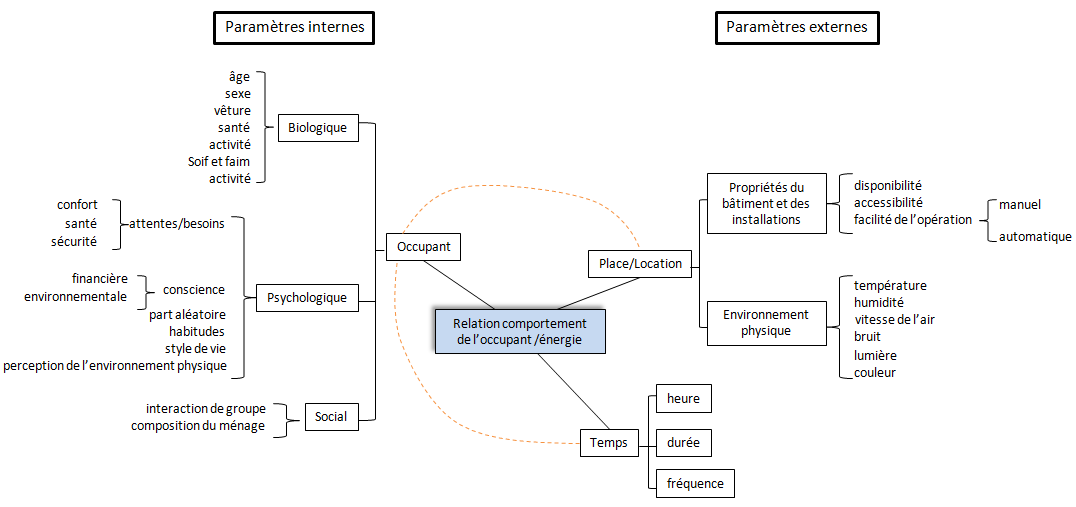
\includegraphics[scale=0.6]{Images/Comportement_occupant_energie}
\caption{Relation entre le comportement des occupants et les consommations d'énergie}
\label{fig:Comportement_occupant_energie}
\end{figure}

\paragraph{Genre}

La Figure \ref{fig:Comportement_occupant_energie} indique que le sexe est un paramètre biologique qui influe sur les consommations énergétiques. En effet, plusieurs études physiologiques ont montré que les femmes et les hommes n'ont pas les mêmes attentes en terme de confort. En effet, Foda et al. \cite{Foda-11} et Jacquot et al. \cite{Jacquot-14} ont montré que les sentions thermales ne sont pas identiques selon le genre, cela modifie donc les températures de consigne et en conséquence les consommations énergétiques. Il a été prouvé que les femmes ont tendance à moins bien supporter le froid que les hommes, alors que ces derniers sont plus vulnérables face aux températures élevées.

\paragraph{Interactions de groupe}

Une communauté scientifique de sociologues de l'énergie se développe afin de mieux comprendre les comportements humains vis à vis de l'énergie et notamment les effets de groupes. Dans ce cadre, des Journées Internationales de la Sociologie de l'Énergie \footnote{Site officiel des deuxièmes JISE 2015 à Tours: \url{http://www.socio-energie2015.fr}} (JISE) s'organisent pour étudier les pratiques courantes des usagers.

Les conflits sur les niveaux de confort dans les bâtiments résidentiels sont fréquents dans tous types de ménages. Les rapports sociaux entre un mari et sa femme, entre des parents sur leurs enfants ou un patron sur ses employés modifient les consommations énergétiques. Certaines relations sont plutôt démocratiques, d'autres sont plus autoritaires, ainsi des règles de priorité peuvent être établies au sein du groupe social. Ainsi, les pratiques liées à l'énergie alimentent un processus de différenciation identitaire entre les membres de la famille: l'un est toujours plus frileux ou économe que l'autre. Aussi, la présence d'invités au domicile est un moment de surconsommation avec des rituels d'accueil (mise en fonctionnement d'appareils de cuisine, augmentation de la température, augmentation de l'intensité lumineuse, musique, etc.) calqués aux normes sociales mais qui participent également à une certaine mise en scène de l'identité familiale.

La définition de règles d'usage et de priorité entre les agents est complexe à définir tant les paramètres d'influence sont nombreux. Alfakara et Croxford \cite{Alfakara-14} dans leurs travaux modélisent les interactions sociales en définissant que l'individu le plus âgé d'une pièce à vivre est celui qui fixera ses conditions de confort ou de volonté, et cela dans un contexte de surchauffe estival. Quelles que soit les règles fixées, il ne faut pas perdre à l'esprit qu'ici l'intérêt est de modéliser les performances et consommations énergétiques plutôt que de modéliser les interactions sociales.

\paragraph{Accessibilité aux systèmes}

Plusieurs études ont montré que lorsque l'on s'intéresse aux actions des occupants dans le bâtiment l'accessibilité aux systèmes de contrôle modifiait les comportements. Sutter et al. \cite{Sutter-06} ont étudié l'utilisation des stores dans les bureaux en fonction de leur accessibilité. Ils en ont conclu que les stores électriques (accessibles à distance) des bureaux étaient trois fois plus utilisés que les stores manuels. Cette étude a été réalisée en observant de l'extérieur le nombre de montées-descentes des stores. 

Andersen \cite{Andersen-09} confirme que l'accessibilité des systèmes de contrôle joue un rôle majeur dans le comportement des usagers et affirme que le temps avant de s'adapter à une zone d'inconfort diminue lorsque les moyens d'adaptation sont nombreux et disponibles. Cette disponibilité des contrôles sur le confort visuel ou thermique modifie alors les comportements adaptatifs des usagers et a en conséquence un impact direct sur le bilan énergétique.

\subsubsection{Aléas}

Nous venons de voir que les comportements humains sont rationnels et qu'ils dépendent de paramètres dits "internes" et "externes". Malgré ces relations plutôt rationnelles entre l'environnement et les actions des occupants, il y a également une part d'insaisissable dans l'humain qui ne réagit pas de manière déterministe à la manière d'un robot. En d'autres mots, un même individu dans un contexte exactement similaire ne réagira pas toujours de la même façon. Les usagers par leurs comportements incertains, rendent les prévisions énergétiques également incertaines. Cette part aléatoire des comportements humains doit ainsi être mieux appréhendée pour l'intégrer aux calculs de performances énergétiques.

Les comportements humains sont donc rationnels et aléatoires. D'après les travaux d'O'Brien et Gunay \cite{O'Brien-14} et de ceux de Leaman \cite{Leaman-99}, les comportements humains sont également parfois surprenants. En effet, ils ont en outre remarqué que certains occupants:
\begin{itemize}
 \item attendent un certain temps avant de s'adapter lorsqu'ils sont en zone d'inconfort
 \item compensent en excès leurs actions à des inconforts mineurs
 \item prennent l'option la plus facile et la plus rapide pour un effet immédiat plutôt que la meilleure 
 \item laissent consciemment ou non les systèmes dans leur état après un changement plutôt que de les réinitialiser après que l'inconfort soit passé
 \end{itemize} 

L'ensemble de ces éléments comportementaux rendent compte de la difficulté d'un exercice de modélisation de l'humain. Néanmoins, la modélisation de ces comportements est une modélisation intermédiaire qui ne sert qu'à améliorer les simulations des bâtiments. Une modélisation fine de l'humain n'apporterait pas spécialement de meilleurs résultats, un optimum de niveau de modélisation est à trouver. En connaissance de cause, nous avons la conviction que modéliser des comportements extrêmement surprenants ou même dérivants, n'améliorerait pas les prédictions énergétiques.

\subsubsection{De la sociologie à l'ingénierie}

Comme nous venons de le voir le comportement des occupants peut se décomposer en une part rationnelle et une part aléatoire. La traduction des études sociologiques en informations exploitables pour des ingénieurs d'études ou de recherche est difficile car les données sont qualitatives plutôt que quantitatives. De plus, ces données sont souvent très disparates et privées de droits. On peut tout de même recenser certains organismes, comme le Centre de Recherche pour l'Etude et l'Observation des Conditions de vie (CREDOC), qui recense quelques données quantitatives sur la façon dont vivent les habitants d'un point de vue social mais également énergétique. 

Dans le but de synthétiser et de catégoriser les paramètres d'influences sur le chauffage, le refroidissement, la ventilation, les opérations sur les fenêtres, l'utilisation de l'eau chaude sanitaire, de l'usage d'électricité et de l'éclairage, l'Annexe 53 \cite{Annex-53-1} a créée des tableaux de synthèse. La Table \ref{tab:drivingforce} présente les niveaux d'importance des paramètres influençant les comportements et la Table \ref{tab:drivingforceheat} est une application pour les comportements vis à vis du chauffage. Le tableau se lit comme: la température de consigne dépend fortement du niveau d'isolation du bâtiment, alors que la durée du chauffage dépend très peu des intentions du gouvernement. L'ensemble des tableaux se trouve dans le rapport final de l'Annexe 53.

\begin{table}[h]
\begin{center}
\begin{tabular}{|c|c|}
\hline
\multicolumn{2}{|c|}{\textbf{Importance}} \\
\hline
\hline Description & Symboles \\
\hline Très hautement significatif ($p\leq 0.001$) & \cellcolor{OliveGreen} *** \\
\hline Hautement significatif ($p\leq 0.01$) & \cellcolor{LimeGreen} ** \\
\hline Modérément significatif ($p\leq 0.05$) & \cellcolor{yellow} * \\
\hline Peu significatif ($p\leq 0.1$) & \cellcolor{orange} ' \\
\hline Pas significatif & \cellcolor{red} p.s. \\
\hline Pas déclaré & \cellcolor{gray} x \\
\hline
\end{tabular}
\caption{Notation utilisée pour l'importance des paramètres influents; la valeur p correspond au niveau statistique}
\label{tab:drivingforce}
\end{center}
\end{table}

\begin{table}[H]
\begin{center}
\small
\begin{tabular}{|p{2cm}||p{2cm}|p{2cm}|p{2cm}|p{1.5cm}|p{2cm}|p{2cm}|}
\hline & Biologique & Psychologique & Sociologique & Temporel & Environnement physique & Bâtiment et équipements \\
\hline
\hline \multirow {3}{1pt}{Consigne de température} & \cellcolor{gray} Genre \cite{Andersen-09} & \cellcolor{yellow} Attentes \cite{Keul-11} & \cellcolor{LimeGreen} Possession (propriétaire, locataire) \cite{Keul-11} & \cellcolor{orange} Heure de la journée \cite{Andersen-09} & \cellcolor{OliveGreen} Température extérieure de l'air \cite{Larsen-10} & \cellcolor{OliveGreen} Niveau d'isolation du bâtiment \cite{Muller-10} \\
\cline{2-7} & \cellcolor{LimeGreen} Habits \cite{Andersen-09}\cite{Keul-11} & \cellcolor{OliveGreen} Fréquence d'interaction avec le système de contrôle \cite{Andersen-09} &  &  & \cellcolor{LimeGreen} Humidité de l'air extérieure \cite{Andersen-09} & \cellcolor{yellow} Type de ventilation \cite{Keul-11} \\
\cline{2-7} &  & \cellcolor{yellow} Ouverture de fenêtre \cite{Andersen-09} &  &  &  &  \\
\hline \multirow {3}{50pt}{Durée de l'activation du chauffage} & \cellcolor{LimeGreen} Habits \cite{Andersen-09}\cite{Keul-11} & \cellcolor{LimeGreen} Compréhension des fonctions de contrôle \cite{Andersen-09}\cite{Keul-11}\cite{Peeters-08} & \cellcolor{Orange} Possession (propriétaire, locataire) \cite{Andersen-09} &  & \cellcolor{OliveGreen} Température extérieure de l'air \cite{Andersen-09} & \cellcolor{OliveGreen} Niveau d'isolation du bâtiment \cite{Muller-10} \\
\cline{2-7} &  &  &  &  & \cellcolor{OliveGreen} Humidité de l'air extérieure \cite{Andersen-09} & \cellcolor{OliveGreen} Type du système de chauffage \cite{Andersen-09} \\
\cline{2-7} &  & \cellcolor{yellow} Ouverture des fenêtres \cite{Andersen-09} & \cellcolor{red} Intentions gouvernementales \cite{Muller-10} &  & \cellcolor{LimeGreen} Vitesse du vent \cite{Andersen-09} & \cellcolor{OliveGreen} Niveau de contrôle \cite{Andersen-09} \\
\hline Nombre de pièces chauffés &  & \cellcolor{OliveGreen} Fréquence des interactions avec les systèmes de chauffage \cite{Andersen-09} &  &  &  & \cellcolor{OliveGreen} Niveau de contrôle \cite{Andersen-09} \\
\hline Pièces chauffés & \cellcolor{orange} Genre \cite{Andersen-09} &  &  &  &  & \cellcolor{OliveGreen} Niveau de contrôle \cite{Andersen-09} \\
\hline
\end{tabular}
\normalsize
\caption{Valeur des paramètres d'influence sur le chauffage de l'espace selon la littérature}
\label{tab:drivingforceheat}
\end{center}
\end{table}


\subsection{Météo}

En phase d'exploitation, la météo, en plus des usages et usagers, modifie les performances des bâtiments. Ce chapitre sera moins étoffé que le précédent car les phénomènes météorologiques sont de notre point de vue suffisamment bien modélisés dans les outils de Simulation Thermique Dynamique (STD). Les températures extérieures, les vents, et les apports solaires sont intégrés dans les calculs de manière dynamique et modifie en phase d'exploitation les consommations énergétiques des bâtiments. La prévision de la météo étant limitée à quelques jours, il n'est pas possible de la prévoir sur la durée de la simulation. Une correction de la simulation en fonction de la météo permet ainsi de ne pas justifier le \textit{performance gap} par des événements climatiques loin des normales.

\section{Maintenance}

Cette section s'intéresse à la maintenance des systèmes des bâtiments et aux systèmes eux même. En prémisse, on peut rappeler la différence entre besoins et consommations énergétiques. Les besoins correspondent à ce qui est nécessaire de fournir aux bâtiments pour qu'ils atteignent les niveaux de confort et performance exigés. Alors que les consommations d'énergie sont égales aux besoins plus les pertes. Lors d'une approche de modélisation bottom-up, ou dite de synthèse, comme une simulation thermique dynamique, prédire les consommations énergétiques nécessite de connaitre d'une part les besoins mais également les propriétés des systèmes. Une bonne efficacité des systèmes est alors essentielle pour réduire les consommations, tout comme une bonne connaissance des rendements est essentielle pour prédire les consommations réelles.

La dégradation des performances des systèmes lors de l'exploitation des bâtiments est alors à considérer pour éviter les dérives de consommations et maîtriser les estimations. Cette dégradation liée à l'usage et à la mise en œuvre des composants est étudiée dans le projet ANR (Agence Nationale de la Recherche) MAEVIA, du programme VBD (Villes et Bâtiments Durables). Bien que ce projet soit prioritairement appliqué à la qualité de l'air intérieur, la simulation du bâtiment dans ses conditions réelles d'utilisation est tout de même fondamentale. En effet, la dégradation des systèmes peut impacter de pair la Qualité de l'Air Intérieur (QAI) et les performances énergétiques. Cette liaison est l'objet d'étude de MAEVIA, qui développe un outil applicable à la QAI pouvant se coupler à un outil de simulation thermique.

Brisepierre \cite{Brisepierre-11}, sociologue de l'énergie a enquêté sur le rapport entre les équipements et les usagers. Il a alors souligné les difficultés qu'ont les occupants à piloter leurs équipements. Cela, entraîne des utilisations non optimales qui réduisent les performances et donc augmentent les consommations énergétiques. Brisepierre a noté que la gestion de la ventilation est particulièrement mal gérée par les occupants alors que son impact sur les consommations énergétiques est très fort. Ici encore une mauvaise gestion automatique ou manuelle du renouvellement d'air a un impact significatif sur le confort et les consommations énergétiques. La connaissance des systèmes, de leurs pilotage et de la sensibilisation qu'ont les occupants de ses systèmes sont autant de paramètres à prendre en considération pour l'estimation des consommations énergétiques. 

\section{Engagement performantiel}

Comme les sections précédentes le laisse comprendre, de nombreux paramètres influencent les performances réelles des bâtiments. Estimer des consommations est alors un exercice complexe, mais qui doit être réalisé avec soin pour que les travaux de constructions ou de rénovations atteignent bien les performances visées. En effet, les travaux à hautes performances énergétiques ne peuvent se réaliser à grande échelle que si les commanditaires des travaux de rénovation énergétique ont la certitude d'obtenir les économies d'énergies vendues et les gains financiers associés.

S'engager dans des travaux de rénovation lourds ou dans des opérations de construction très performantes implique un risque fort pour les donneurs d'ordre. Afin de les rassurer sur l'efficacité réelle de tels travaux il existe des CPE (Contrats de Performance Énergétique), dont la fondation Bâtiment-Énergie \cite{FBE-16} est à l'origine et qui propose un guide d'accompagnement sur l'élaboration d'une méthodologie de GRE (Garantie de Résultats Énergétiques). Ces contrats visent à sécuriser les actions de l'ensemble des acteurs pour garantir des résultats. Ils proposent aux co-contractant de se mettre d'accord sur une GPE (Garantie de Performance Énergétique) couvrant telle ou telle partie de la vie d'un bâtiment. La GRE est la forme la plus complète de GPE de la conception à l'exploitation d'un bâtiment. La GRE garantit au donneur d'ordre que la consommation, après travaux et ajustements éventuels ne dépassera pas une certaine valeur. En cas de non atteinte de la garantie et en fonction des termes de contrat, les responsabilités sont recherchées afin de dédommager le client. Ce travail contractuel concerne les travaux de rénovation mais également les bâtiments neufs, pour lesquels les moindres consommations d'énergie annoncées doivent être sécurisées, en regard des investissements complémentaires consentis.

Les prestataires par une GRE mobilisent une partie du gisement d'économies d'énergie qui n'avaient pas été exploitée pour des raisons techniques, financières ou organisationnelles par le consommateur final. Engager des travaux de rénovation revalorise le patrimoine et contribue à rembourser l'investissement initial et donc à réduire les coûts d'exploitation.

Cette section présente sous les angles, juridique, financier, technique et méthodologique, la mise en place d'un engagement contractuel sur la performance énergétique sécurisant et rentable.  

\subsection{Juridique}

L'introduction sur l'engagement contractuel a permis de présenter l'intérêt de développer la contractualisation de performance énergétique car elle permet de mieux concevoir, de mieux réaliser, de mieux exploiter et de mieux communiquer sur les opérations. L'engagement permet d'assurer l'économie du projet pour le maître d'ouvrage et les utilisateurs en répartissant les gains ou en pénalisant les fautifs. 

D'un point de vu juridique, il est essentiel de définir les porteurs de l'engagement. La législation actuelle est souple et laisse la liberté aux co-contractants de négocier leurs limites d'interventions et donc de responsabilités. Quel que soit l'acteur qui porte l'engagement (la maîtrise d'ouvrage, la maîtrise d'œuvre, l'exploitant ou une tierce partie), il possède un droit d'intervention sur l'ensemble des autres acteurs qui ont un lien avec la performance énergétique.

La fondation Bâtiment-Énergie \cite{FBE-16} préconise quatre schémas de contractualisation possible selon le degré d'implication, de capacité et de compétence du donneur d'ordre. Dans le schéma 1, la GRE est portée à 100\% par un prestataire qui intervient dès les premières phases du projet, c'est à dire lors de la phase d'audit pour les travaux de rénovation. Le schéma 2, le plus utilisé, implique davantage le donneur d'ordre en lui confiant l'audit énergétique et la programmation performantiel prévisionnel, un prestataire s'occupe ensuite d'identifier et de tester les gains potentiels puis propose un engagement tenable. Le schéma 3 est semblable au 2 avec cependant un niveau de définition des solutions plus avancé par la maîtrise d'ouvrage. Dans cette configuration, le prestataire se voit réduire sa palette de solutions pour atteindre l'objectif. Le dernier schéma juridique rend la garantie de résultats énergétiques à la maîtrise d'œuvre qui porte l'engagement contrairement aux 3 précédant schémas qui est porté par une entreprise de service énergétique. 

Finalement, le choix du schéma par le donneur d'ordre dépend principalement de ses compétences. Malgré cela, le schéma 1, plus cher car moins impliquant pour le donneur d'ordre, ne l'affranchit pas d'un suivi précis des phases du contrat et d'un accompagnement du prestataire ou du maître d'œuvre.

\subsection{Financier}

L'aspect financier des projets de GPE est fondamental car il dicte les choix des donneurs d'ordres. L'angle financier pris dans cette section ne considère que les sources de financement et deux indicateurs de l'estimation de la rentabilité des projets.

Par essence, un contrat de performance énergétique garantie une réduction des consommations énergétique et donc des dépenses moindre à la suite de projets de rénovation énergétique. Les économies sont évidement effectives qu'après l'achèvement des travaux puis durent pendant toute la phase d'exploitation. Une deuxième source de financement un peu particulière concerne les Certificats d'Economie d'Energie (CEE). A la suite de travaux d'amélioration de performance énergétique, il est possible de demander ces CEE qui sont monnayables auprès d'un fournisseur d'énergie. Après validation, le prix de l'énergie consommé sur le site se retrouve diminué. La troisième source de financement et la plus évidente concerne les fonds propres de l'investisseur. Bien sûr, nous pouvons également considérer la revalorisation patrimoniale et la valeur verte comme valorisant les bâtiments rénovés, cela n'est pas une source de financement à proprement parlé, mais est entièrement considéré par les donneurs d'ordres. Enfin, dans le cas où les fonds propres et autres aides ne sont pas suffisants, les donneurs d'ordres peuvent faire appel à un tiers financement. Le financeur prête alors au donneur d'ordre qui le remboursera en phase d'exploitation en intégrant une partie des économies réalisées grâce aux améliorations énergétiques.

Concernant ce tiers financement des Sociétés Publiques Locales (SPL) comme la SPL d'efficacité énergétique OSER\footnote{Site internet \url{http://spl-oser.fr/}} de la région Rhone-Alpes ou la Société d'Aménagement et d'Equipement de la Région Parisienne (SAERP)\footnote{Site internet \url{http://www.saerp.fr/}} proposent de prendre en charge l'ensemble des étapes des projets avec les collectivité de la région, notamment financier. Ce type de structure en plein essor propose des actions transversales en se faisant déléguer le travail de maîtrise d'ouvrage des collectivités par la signature d'un Bail Emphytéotique Administratif (BEA). Les SPL font appel à des fonds d'investissement et négocient les conventions de prêts, puis négocient les CPE avec les entreprises locales. Cette prestation est dans cet exemple à destination des collectivités locales, mais est également applicables pour assister des maîtres d'ouvrages en copropriétés ou dans le tertiaire.

En plus du financement initial du projet de GRE, le donneur d'ordre doit estimer la rentabilité financière du projet. Pour ce faire il peut raisonner en rendement brut de l'investissement, c'est à dire en évaluant le rapport économie annuelle suite aux travaux de rénovation sur l'investissement total. Le temps de retour sur investissement est le deuxième indicateur que nous pouvons citer pour évaluer la rentabilité d'un projet, c'est la durée nécessaire pour que l'investissement total soit remboursé grâce aux économies annuelles. Lorsque le donneur d'ordre réalise ce type de calcul il est important qu'il considère les frais financiers (actualisation) et l'évolution prévisionnelle du prix de l'énergie.

\subsection{Technique}
\label{Engagement performantiel - Technique}

Les Contrats de Performance Energétique (CPE) impliquent à certains acteurs de la conception et construction de prévoir les futures consommations. L'Institut Français pour la PErformance des Bâtiments (IFPEB) \cite{IFPEB-2014} propose un guide construit autours de quatre piliers essentiels pour s'engager sur des futures consommations. Avant de présenter ces piliers, il est important de sensibiliser les donneurs d'ordre sur l'intérêt des démarches intégrées comme les contrats Conception / Réalisation / Exploitation / Maintenance (CREM) qui permettent de réduire l'effet de rupture technique à la livraison, l'exploitant ayant participé activement à la conception puis s'étant engager sur un contrat de performance énergétique.

Le premier pilier et peut être le plus fondamental est de bien définir les usages, l'intensité d'usage et le potentiel d'usage du bâtiment, qu'il soit neuf ou en rénovation. Orienter la conception côté utilisateur est un gage de confort qui a parfois tendance à être délaissé lors de la course à la performance énergétique. Néanmoins, dans le cycle de vie d'un bâtiment plusieurs usages y ont lieu, il faut donc construire des bâtiments robustes qui ne verront pas leurs consommations dériver pour un certain type d'usage.

Le second pilier et celui qui nous intéresse le plus dans ce manuscrit de thèse consiste à prévoir les futures consommations énergétiques tous usages compris. Le premier pilier servant à définir un usage nominal mais également des potentiels d'usages, la Simulation Energétique Dynamique (SED) de l'opération doit également prendre en considération les différents usages du bâtiment. Cette approche est également défendu par Lenormand \cite{Lenormand-15} qui prône une approche des SED par les tangentes plutôt que par les ponts, c'est à dire où l'énergéticien réalise des simulations dans des situations extrêmes qui lui permettent de tester la flexibilité des opérations. Cette approche de simulation permet alors de tester des comportements, scénarios ou situations extrêmes, mais ne permet pas de prédire des performances dans un intervalle de confiance. Pour cela, il est nécessaire de réaliser plusieurs simulations en faisant varier un certain nombre de paramètres afin de réaliser une analyse de l'incertitude. Comme nous l'avons évoqué en introduction, les paramètres les plus incertains lors des simulations des bâtiments sont ceux relatifs aux occupants. Cette incertitude est propre aux comportements des humains, d'où le développement de modèles stochastiques à base d'agents de ce travail de thèse. La simulation multiple permet alors d'obtenir en sortie de SED une densité de probabilités des consommations énergétiques, plutôt qu'une valeur unique qui n'apporte pas d'indication sur la flexibilité intrinsèque du bâtiment.

Le troisième pilier de l'IFPEB, que nous reprenons également ici, concerne la mesure et la vérification de la performance énergétique, communément appelé Plan de Mesure et de Vérification (PMV), ainsi qu'une supervision énergétique. Une fois le bâtiment livré, il faut mesurer les consommations réelles en les ajustant aux conditions météorologiques et d'usages, cela permet de vérifier si les consommations prédites étaient bonnes. Si, c'est le cas alors le contrat est rempli pour le porteur de l'engagement, si ce n'est pas le cas alors une investiture est menée pour comprendre et réparer les défaillances. Ces défaillances peuvent être de diverses natures et peuvent mener soit à de nouveaux travaux, soit à un travail d'Assistance à Maîtrise d'Usage (AMU) auprès des occupants ou soit à des dédommagements si les deux premières solutions sont infructueuses. En cas de non atteinte des performances visées, les co-contractants doivent se référer à leurs Contrat de Performance Energétique pour les dédommagements. Ce pilier est donc nécessaire pour vérifier les clauses du CPE, mais est surtout un atout technique pour améliorer la performance énergétique des bâtiments et atteindre le facteur 4 généralement visé par une réhabilitation énergétique lourde ou une opération neuve exemplaire.

Le dernier pilier consiste à réduire le risque de non atteinte des objectifs sur toute la durée du projet, c'est ce que nous appelons le \textit{commissioning} ou supervision en français. Cette supervision est finalement extérieure au projet et fait la synthèse des trois autres piliers décrits auparavant. Il s'assure donc en début de projet que les exigences du donneur d'ordre en terme énergétique ont été appropriées par la maîtrise d'œuvre. En phase d'études le \textit{commissioning} assiste l'équipe de conception puis assiste les entreprises en phase de travaux. Avant la livraison du bâtiment, il s'assure de la conformité des différents tests, tels les tests d'étanchéité à l'air, puis s'assure de la bonne prise en main du bâtiment par l'exploitant après livraison. Cette prise en main concerne donc d'une part le travail de suivi énergétique dans le cadre du troisième pilier et d'autre part la connaissance des systèmes et des opérations de maintenance à prévoir. 

\subsection{Méthodes}

Le développement de la méthodologie de projets de Garantie de Résultats Energétique (GRE) modifie le schéma de conduite de projet et de contractualisation habituels. Le constat de la méthodologie actuelle montre un écart significatif entre performance théorique et réelle dû à la linéarité des étapes du projet de construction et surtout à la contractualisation habituelle qui fixe des objectifs techniques constructifs et des obligations de moyens. Contrairement à l'approche classique, la méthodologie de la GRE permet une définition plus précise du niveau réel de performance atteignable en considérant les retours du terrain et en adoptant un processus d'affinement du tunnel de risque.

Ce tunnel de risque a vocation à se rétrécir au fur à mesure de l'évolution des phases du projet et de l'identification des améliorations de la performance énergétique en ce qui concerne la rénovation énergétique. Lorsque le choix des travaux ou de bouquet de travaux est définit, l'équipe de conception peut alors prédire une consommation assez finement si l'usage est connu.

Une fois le bâtiment livré avec les améliorations de performance énergétique, la moitié du travail reste à réaliser. La fondation Bâtiment-Énergie \cite{FBE-16} nomme cette seconde étape le processus bouclé en phase d'exploitation. En mesurant la performance ajustée aux conditions réelles d'exploitation du bâtiment et en la comparant à la performance prédite et garantie, et en cas de différence trop importante il doit être possible de corriger l'exploitation ou revoir les travaux réalisés. Cette méthodologie permet ainsi d'atteindre le niveau de performance visé en ajustant les dispositifs ou en accompagnant les occupants sur les bonnes pratiques. Si les ajustements ne sont pas suffisants alors les pénalités juridiques et financières prévues peuvent s'appliquer à l'encontre des fautifs.

La GRE n'est pas le seul type de Contrat de Performance Énergétique (CPE), il existe également la Garantie de Performance Énergétique Intrinsèque (GPEI) qui se limite au stade de la conception et assure la performance intrinsèque du bâtiment et des équipements sans considérer l'usage. Ce type de contrat est moins contraignant pour les donneurs d'ordre et co-contractants car il n'est pas engageant sur la durée d'exploitation. Ce type de contrat bien que de plus en plus utilisé n'est pas présenté dans ce manuscrit, car il ne considère pas les usages: sujet majeur de cette thèse.

Nous pouvons rappeler que l'engagement performantiel est bien une nouvelle méthode de travail pour les concepteurs, mais qui implique des coûts supplémentaires quelque soit le type d'opération. En effet, bien entendu la non-qualité est très chère, mais l'ultra perfection l'est également, un point d'équilibre existe. Le critère de décision principal pour réaliser ou non un projet de GRE repose sur l'équilibre entre ce coût supplémentaire et le gain en termes de réduction du risque lié à l'investissement. L'engagement contractuel sur le résultat est un mécanisme souhaitable en cas de rénovation énergétique lourde ou en cas de construction neuve ambitieuse, pour assurer l'économie du projet pour la maîtrise d'ouvrage et les utilisateurs. 

\section{Synthèse}

Le doute sur la représentativité des modèles doit se poser et la citation de Baudrillard: "La simulation précède le réel" sans que "le simulacre remplace l'original" résume bien l'état d'esprit. En partant du constat que les performances énergétiques mesurées sont souvent éloignés de la théorie, nous avons dans ce chapitre évoqué les facteurs pouvant expliquer ces écarts. Le comportement des occupants est identifié comme un paramètre essentiel mais aujourd'hui mal pris en compte dans la modélisation. En effet, les méthodes de simulations actuelles utilisent souvent des scénarios hebdomadaires répétitifs pour simuler l'action des usagers sur le bâti. La prise en compte des apports internes, les positions des protections solaires, la régulation des aérations sont des exemples décorrélés de la notion de confort. Une nouvelle approche doit permettre de développer un modèle, dans lequel les utilisateurs ne sont plus aussi prévisibles et passifs, mais interagissent entre eux et sur leur milieu, modifiant certains paramètres de la simulation en fonction de leurs besoins et activités réelles. Ainsi, les phénomènes d'actions et réactions entre les utilisateurs et leur environnement, pourront mieux être intégrés aux simulations numériques.

La prise en compte de ces phénomènes permettra entres autres de ne plus obtenir comme résultat d'une étude une consommation énergétique absolue, mais plutôt une fourchette basse et haute permettant de connaître la sensibilité du bâtiment à une utilisation plus ou moins vertueuse de celui-ci.
\chapter{Modélisation du comportement des usagers}

La démarche de modélisation est une approche scientifique qui a pour but de produire de la connaissance sur des phénomènes naturels ou artificiels. Cette démarche est utilisée pour comprendre, prédire voire contrôler des phénomènes qu'ils soient déjà existants ou encore au stade de la conception. Le principe est de créer une simplification numérique du phénomène étudié. Les modèles sont donc souvent indispensables, mais ils sont également toujours faux. Les bons modèles sont des approximations qui apportent une plus-value pour la prévision de phénomènes.

Cette thèse s'intéresse à la modélisation du comportement des occupants pour la prédiction de la demande d'énergie. Pour cela, il est nécessaire de s'intéresser à l'interaction entre les occupants et leur environnement. Ces interactions sont de deux natures: la première concerne les gains dus aux apports métaboliques et les divers apports internes de chaleur; la seconde concerne l'utilisation des systèmes de l'environnement (fenêtres, volets, lumières, air conditionnée, etc.) qui sont régulés par les occupants et leurs besoins.

Réussir à modéliser les actions et comportements des usagers d'une manière cohérente et généralisée est important pour offrir aux industriels des méthodes et des logiciels adaptés à leur mission de conception de bâtiment. Ce chapitre présente alors les types de modélisation du comportement des occupants recensés dans la littérature et les plateformes numériques pouvant réaliser ces modélisations. 

\section{Types de modèles}

Il existe deux grands types d'approche de modélisation, les approches descendantes (dites \textit{top-down} en anglais) et les approches ascendante (dites \textit{bottom-up} en anglais). Les modèles de demande d'énergie descendants comme celui qu'a développé Kelly et al. \cite{Kelly-13} utilise une analyse de régression d'une grande population pour déterminer l'influence des facteurs individuels. Alors que les modèles ascendants étudient en détails chaque composant pour les combiner et générer un résultat d'ensemble. C'est ce deuxième type d'approche qui est traité dans la suite de ce chapitre.

Au sein de ce type d'approche, nous avons réalisé une étude bibliographique qui nous a permis de distinguer six familles de modélisation du comportement des usagers à des fins énergétiques dans le contexte du bâtiment. Cette large revue des modèles existants est indispensable pour en comprendre les possibilités, forces et faiblesses de chacun afin de répondre aux objectifs initiaux. Les modèles dits: psychologiques, basés sur des valeurs moyennes, déterministes, probabilistes, utilisant les systèmes multi-agents et "action-based" sont présentés dans ce qui suit.

\subsection{Modèles psychologiques}

Les modèles psychologiques du comportement des occupants peuvent être distingués en deux groupes, ceux considérant le comportement individuellement et ceux en lien avec l'utilisation de l'énergie dans les bâtiments.

En effet, certains modèles psychologiques fonctionnent en utilisant comme indicateurs les besoins fondamentaux des êtres humains. Ces derniers se limitent d'une part aux besoins physiologiques des êtres humains: faim, soif, sexualité, respiration, sommeil, élimination selon la pyramide établie par le psychologue Maslow \cite{Maslow-56}. D'autre part à la notion de confort physiologique qui considère les aspects hygrothermiques, acoustiques, visuels et olfactifs. Dans un cadre de modélisation du comportement des usagers à des fins énergétiques, il va de soi que l'intégralité de ces besoins et types de confort ne sont pas pris en compte. 
Une fois les définitions des paramètres d'influences sélectionnés, l'objectif est de prédire les pratiques \footnote{En langue française on utilise comme synonyme "pratique" et "comportement" alors que la langue anglaise fait une distinction sémantique. "Behavior" désigne un geste observable et quantifiable, alors que "practice" renvoie à l'activité et permet d'insister sur son contexte de réalisation comme sur le sens que les individus lui attribuent} des usagers en fonction de la physiologie de la population et des normes sociales. En 1991, le psychologue social, Ajzen \cite{Ajzen-91}, a mis au point une théorie du comportement planifié de ce type, qui s'est révélée comme étant à l'origine de nombreux sous-modèles psychologiques. On y retrouve ces sous-modèles sous forme de boucles, généralement considérant connaissance, désir, capacité, attitude et finalement action. Ce terme de boucle est utilisé dans le sens où le modèle se présente comme un enchainement d'étapes qui sont répétées à chaque pas de temps de la simulation, comme un algorithme.

On a vu que certains modèles psychologiques sont uniquement basés sur la physiologie des occupants, alors que ce paragraphe consacré au deuxième type de modèles psychologiques, intègre la dimension économique. On retrouve une application dans le secteur résidentiel avec Van Raaij et al. \cite{VanRaaij-83} qui prennent soin de considérer le ménage lui-même, c'est à dire son niveau socio-démographique, son style de vie, le prix de l'énergie ou encore sa responsabilité devant l'énergie. En comparaison, aux modèles uniquement basés sur la physiologie, ces modèles se revendiquent comme plus complets car ils considèrent en outre la technologie, l'économie, la démographie, les institutions, la culture. Néanmoins, le principe de boucle n'est pas modifié et l'indicateur principal reste le bien être des occupants. Ici l'approche est plus transversale car elle n'est pas centrée uniquement sur la physiologie de l'occupant et son bien être mais considère également des paramètres qui influent effectivement sur le comportement.

\subsection{Valeurs moyennes}

Les modèles fondés sur des valeurs moyennes sont généralement considérés comme élémentaires par la communauté scientifique car leur flexibilité est très réduite. En effet, pour les différentes entrées du modèle on a des valeurs uniques. C'est donc sur ce principe que se base ce type de modélisation, si l'on cherche à étudier la sortie $y$ d'un phénomène, les entrées $x_1$, $x_2$, $...$ et $x_n$ sont des valeurs statiques, constantes au cours de la simulation. A titre d'exemple, Morel et Gnansounou de l'Ecole Polytechnique de Lausanne \cite{Morel-09} considèrent les gains internes des bâtiments résidentiels égaux à 5$W/m^{2}$. Ici la valeur importe peu, elle est d'ailleurs peut être proche de la réalité, mais sa limite réside dans l'impossibilité de la détailler selon des paramètres d'influence: type de pièce, nombre d'occupant, date et heure, etc. Cet exemple parmi tant d'autres permet de dire qu'un modèle basé sur des valeurs moyennes utilise des données totales comme paramètres d'entrée. Ces types de modèles fonctionnent alors sur l'implémentation de valeurs uniques dans l'algorithme de simulation, par conséquent, il en résulte automatiquement des valeurs également uniques pour chaque sortie.

L'application des modèles basés sur les valeurs moyennes est la plus appropriée pour estimer des consommations énergétiques d'un échantillon large de bâtiments. Comme nous le verrons dans les prochains paragraphes et alors qu'elle est également envisageable pour des bâtiments individuels, des modèles stochastiques ou à base d'agents produiront des résultats moins bruts, plus proches des pratiques possibles et seront donc plus appropriés à un niveau de modélisation supérieur.

\subsection{Modèles déterministes}

Les modèles déterministes ont pour habitude d'être assimilés aux modèles des valeurs moyennes, dans le sens où leurs données d'entrée sont discutables car souvent basées sur des simplifications. Ces suppositions sont le fruit d'études sociologiques quantitatives trop peu nombreuses pour avoir une base de données suffisamment importante et fiable. Certaines données sont disparates et fiables mais tout de même à exploiter avec précaution, tant les paramètres d'influence sont nombreux.

Dans leur modèle, Glicksman et Taub \cite{Glicksman-97} cherchent à identifier les paramètres qui ont la plus grande influence sur l'efficacité énergétique. Dans cet article, la modélisation du comportement des habitants face au chauffage, à la ventilation et à l'air conditionné est faite de manière déterministe. Ce type de modèle simplifié et limité par son dynamisme est également utilisé dans l'outil de simulation thermique dynamique développé par Izuba, Pleiades+Comfie. Dans celui-ci, son cœur de calcul est pour l'utilisateur une boite noire, qui est seulement maître des données d'entrée. Après avoir renseigné le logiciel sur les éléments géométriques, environnementaux et les différents systèmes du bâtiment, le modélisateur doit définir de multiples scénarii d'utilisation. Pour chaque zone thermique, il doit déterminer: les consignes de température, les scénarii d'occupation, les puissances dissipées, les jeux d'occultation, les niveaux d'éclairement ou encore les besoins en eau chaude sanitaire. Cette détermination est réalisée heure par heure au travers de scénarii hebdomadaires répétitifs totalement décorrélés de la notion de confort. Or, on comprend la limite de considérer les comportements des usagers comme entièrement prévisibles et répétables.

\subsection{Modèles probabilistes}

Les processus probabilistes, également appelés stochastiques, utilisent des paramètres et équations qui évaluent les probabilités d'une action ou d'un changement d'état du système. Contrairement aux modèles basés sur des moyennes ou aux modèles déterministes, les modèles probabilistes se basent davantage sur des études statistiques qui proposent des profils. Les méthodes d'échantillonnage de distributions d'événements sont nombreuses. On retrouve fréquemment des méthodes de la transformée inverse, tel que dans le travail de Vorger sur l'influence des occupants sur la performance énergétique par le biais d'une modélisation stochastique globale \cite{Vorger-14} ou des méthodes de Monte-Carlo par chaînes de Markov, comme Tijani l'a fait pour le développement d'un modèle purement statistique \cite{Tijani-14} afin de le comparer aux systèmes multi-agents qui sont eux présentés dans la Section \ref{Systèmes Multi-Agents}. Dans le cadre de la modélisation du comportement, l'approche probabiliste permet de considérer les aléas comportementaux des humains. Cette approche demande de posséder une base de données suffisante pour connaitre les habitudes des occupants, d'où l'intérêt de campagnes de mesures et de questionnaires. Ces informations sur les habitudes des occupants concernent les tâches qui sont réalisées, leurs durées et leurs enchaînements. Les chaines de Markov sont alors le système mathématique qui correspond le mieux à ce besoin. En effet, les processus de Markov sont "sans mémoire" et permettent des transitions d'états pour des durées plus ou moins longues. Ils permettent ainsi de réaliser aléatoirement des changements d'états (positions, actions, activités, etc.) des occupants du modèle en intégrant préalablement les études statistiques. Concrètement, les chaines de Markov de premier degré fonctionnent de la manière suivante:
\begin{enumerate}
\renewcommand{\arraystretch}{0}
\item Étude des données temporelles d'activité, les probabilités cumulées de transition sont calculées
\item La matrice de probabilité de transition est calculée
\item Un nombre aléatoire compris entre 0 et 1 est généré
\item Le nouvel état est déterminé, en fonction de l'état précédent, du nombre aléatoire généré et des probabilités cumulées de transition
\end{enumerate}
Un modèle probabiliste avancé est développé dans le volume II: "Occupant behavior and modeling" de l'Annexe 53: Total energy use in buildings" \cite{Annex-53-1}, celui-ci présente une étude statistique préalable sur les consommations énergétiques, détermine la typologie du bâtiment et détermine les informations sur les occupants afin d'en sortir les localisations et activités de chaque occupant pour un pas de temps de 5 minutes. On notera tout de même que les sorties de ce modèle se limitent ici à la localisation et aux activités des occupants, alors qu'on peut imaginer que la finalité d'un tel modèle sera d'estimer les besoins énergétiques. Les modèles probabilistes et les méthodes de type aléatoire permettent de générer des événements ou échantillons extrêmes, tout en ayant conscience de la pondération des  résultats. En effet, c'est le principe de la Gaussienne, il est plus probable de générer un événement dans la moyenne qu'un événement extrême. En revanche, sur de nombreuses simulations les chaînes de Markov ressemblent à des modèles basés sur des valeurs moyennes, car les moyennes des événements aléatoires vont tendre vers les états les plus fréquents trouvés lors de l'étude statistique \cite{Annex-53-1}.

Pour synthétiser ce qu'est la modélisation stochastique on dit souvent qu'elle égale à une modélisation déterministe associée à une part d'aléatoire.

\subsection{"Action-based" modèles}

Les modèles axés sur les actions des occupants sont développés suivant deux volets: l'occupation des zones et les activités de leurs occupants. Dans ce type de modèle l'occupation est déterminée par la localisation des occupants qui est le résultat des mouvements d'une zone du bâtiment à l'autre. Tout comme pour les modèles probabilistes, ces déplacements d'une zone à l'autre sont généralement générés simplement par les méthodes des chaines de Markov et transitions d'états. Les activités des occupants sont générées aléatoirement et concernent les ouvertures de fenêtres, la gestion des lumières, de l'air conditionné ou encore de l'usage des appareils électroménagers. Ces modèles dits d'actions associent donc les comportements des usagers à des déplacements et à des actions concrètes sur les systèmes du bâtiment.

Comme pour les modèles stochastiques, la typologie des bâtiments, le nombre et les types d'occupants par zone sont renseignés au modèle pour le volet des déplacements des occupants. Cependant, la plus-value réside dans l'ajout d'informations supplémentaires concernant les horaires et durées des séjours et activités dans les zones étudiées \cite{Annex-53-1}. Cette modélisation des déplacements au sein du bâtiment, fixe ou suit l'évolution des systèmes à chaque pas de temps qu'ils soient booléens, discontinus ou continus. Pour les définitions des événements on note généralement six attributs à renseigner au modèle, les temps de début et fin, la localisation, les participants, les indicateurs statistiques et les priorités en cas de conflit. 

Comparés aux modèles déterministes où les actions sont prédéfinies et inchangeables, ces types de modèles considèrent le caractère aléatoire par une occupation inégale et asynchrone dans l'espace et le temps. On a une combinaison entre les modèles déterministes et probabilistes. La plus-value de ce modèle réside dans la personnalisation des occupants, même extrêmes, aussi bien dans leur génération que dans leurs comportements concrets devant les systèmes consommateurs d'énergie. Cependant, les modèles d'actions sont de type réactifs et ne prennent pas en compte les interactions entre les occupants du modèle.

\subsection{Systèmes Multi-Agents (SMA)}
\label{Systèmes Multi-Agents}

Les Systèmes Multi-Agents permettent d'établir des règles de comportement des usagers à travers de l'utilisation d'agents autonomes dont leur comportement est automatiquement calculé sans suivre des profils préétablis. Les modèles à base d'agents considèrent les occupants comme des entités individuelles capables de prendre des décisions selon leurs règles et expériences en étant interactif entre eux et avec leur environnement.

En réalité cette définition complexe est finalement assez souple et plusieurs niveaux d'agents sont généralement perçues. Ferber \cite{Ferber-95} classe les SMA en deux grandes catégories; la première est celle où les agents sont réactifs et reposent sur des actions prédéfinies et déclenchées automatiquement, tels des stimulus. Ces agents réactifs perçoivent leur environnement et agissent sur celui-ci en choisissant parmi des comportements prédéfinis, celui qui est les plus adapté à la situation. La deuxième catégorie de SMA est celle fonctionnant sur des agents cognitifs. Dans cette catégorie les agents possèdent des capacités de raisonnement et de mémorisation. Les agents les plus évolués peuvent même développer de nouvelles connaissances ou des organisations selon des paramètres sociaux, psychologiques et biologiques mais également en fonction des interactions avec les autres agents.

Dans le cadre de la modélisation des occupants dans le contexte du bâtiment et de la maitrise de l'énergie, Davidsson et Boman \cite{Davidsson-05} présentent un modèle multi-agents considérant lumière et chauffage. L'énumération suivante présente les relations simplifiées entre les agents et les conditions intérieures:
\begin{enumerate}
\renewcommand{\arraystretch}{0}
\item Quand aucun agent est dans la pièce, les conditions par défaut sont maintenues
\item Quand un agent entre dans la pièce, il adapte la température et allume les lumières selon ses préférences
\item Quand plusieurs agents sont dans la pièce, les conditions sont fixées en fonction des préférences des agents présents par délibération
\end{enumerate}
Davidsson et Boman \cite{Davidsson-05} utilisent bien des SMA, car les occupants sont assimilés à des agents autonomes aux propriétés individuelles qui leurs sont propres et qui plus est avec des interactions entre eux. Ces agents ne sont en revanche pas cognitifs puisqu'ils n'ont pas de capacité d'apprentissage et de mémorisation, c'est à dire qu'ils sont davantage pulsionnels qu'intentionnels.

Kashif \cite{Kashif-11} a quand à elle développé sous BRAHMS \footnote{BRAHMS est un logiciel développé par la NASA, permettant la simulation et l'analyse séquencée du comportement des agents lors de chaque processus de décision} des agents cognitifs ayant une perception de leur environnement et une capacité de délibération pour le contrôle et la gestion de l'énergie. Dans ce projet les mécanismes de réaction aux évènements prennent en compte une explicitation des buts, des mécanismes de planification et peuvent résoudre des problèmes qualifiés de complexes. Cette approche choisie par Kashif considérant les croyances, les désires, les contraintes, les perception et les états physiques mobilise une partie de la branche de l'intelligence artificielle en laissant apercevoir un potentiel jugé fort. Or à l'heure actuelle cette approche très fine ne permet pas d'avoir des résultats d'ensemble exploitables notamment en termes de consommations énergétiques. Tijani \cite{Tijani-14}, dans la continuité du travail de Kashif \cite{Kashif-11}, dans son article sur l'approche multi-agents du comportement des occupants avertit et confirme que malgré un fort potentiel des SMA, la complexité de BRAHMS rend l'application à l'énergétique des bâtiments et à la qualité de l'air intérieur difficile.

En plus des niveaux de détails des modèles qui dépendent des objectifs des projets, les disciplines insistent sur différents aspects du processus de décision humain:
\begin{itemize}
\renewcommand{\arraystretch}{0}
\item En psychologie, les agents sont créés autours de facteurs internes tels les croyances et désires. Soit les agents réagissent selon les théories d'actions normalisées de Schwartz \cite{Schwartz-77} ou soit selon les théories de comportement planifié d'Ajzen \cite{Ajzen-91}.
\item En économie, les agents sont créés autours de facteurs externes tels des indices du marché et autres aspects financiers. Ce sont ces paramètres rationnels économiques qui vont guider les décisions des agents.
\item En informatique, les agents sont créés à partir des connaissances de l'intelligence artificielle et propose des capacités évoluées d'autonomie. Savall \cite{Savall-03} au travers de son modèle d'organisation YAMAM montre comment la cognitivité est recherchée notamment par la possibilité de modifier des règles de comportement des agents en cours de simulation.
\end{itemize}
Ainsi, plusieurs sciences utilisent les Systèmes Multi-Agents à des fins diverses et aux niveaux de complexité et cognitivité hétéroclites. Les conditions communes minimales pour appeler les agents comme tels selon trois précurseurs des SMA: Erceau \cite{Erceau-93}, Ferber \cite{Ferber-95} et Maes \cite{Maes-95} sont de percevoir l'environnement, de décider selon des perceptions, puis d'agir sur l'environnement. 

\subsection{L'approche hybride socio-stochastique}

1- Utilisation des modèles stochastiques utilisés couramment lors de la modélisation des comportements des occupants.
- Méthode de la transformée inverse (Eric Vorger p37)
- Modèle linéaire multiple
- Chaines de Markov à temps discret 
- Analyse 

2- Intégration des phénomènes sociologiques en sortie des modèles stochastiques:
- Effet rebond
- Dynamique de groupe 
(- Contournement technologique) G. Brisepierre

\subsection{Synthèse}


%%%%%%%%%%%%%%%%%%
% Fit-to-purpose %
%%%% Gaetani %%%%%
%%%%%%%%%%%%%%%%%%
% Methodology:
% 1. What are the existing models/simulation frameworks for OB?
% 2. Which combination of factors influence the impact of OB on the predicted building energy performance?
% 3. What is the most fit-for-purpose OB modeling complexity level for a specific case 

Le choix du modèle dépend fortement des objectifs de la simulation mais aussi des logiciels choisis ou disponibles. On note que le développement d'un modèle se réalise souvent en couplant plusieurs modèles de base. Dans le tableau \ref{synthese modeles}, sont regroupés les six modèles présentés dans ce chapitre, leurs données d'entrée, leur développement, une référence et enfin les limites générales du modèle considéré. 

\begin{landscape}
\begin{table}
\centering
\begin{tabular}{|p{4.5cm}||p{4.5cm}|p{4.5cm}|p{4.5cm}|p{4.5cm}|p{4.5cm}|}
\hline Type de modèle & Données d'entrée & Développement & Exemples et références & Limites \\
\hline
\hline Modèles psychologiques & Besoins physiologiques, \newline niveau de confort, \newline données économiques & Développement d'algorithmes axés autour d'indicateurs physiologique des usagers & \cite{VanRaaij-83} En plus de l'aspect physiologique, l'aspect social est considéré dans ce modèle psychologique précurseur & Difficulté de la transcription des données sociales en comportements concrets  \\
\hline Valeurs moyennes & Valeurs moyennes fixes (et écarts types), \newline dépend des besoins du modèle & Approche bottom-up - \newline utilisation des inputs dans le cœur de calcul & \cite{Morel-09} Les gains internes sont assimilés à une valeur unique constante & Flexibilité des données d'entrée, \newline non variable dans le temps \\
\hline Modèles déterministes & Scénarios hebdomadaires et annuels répétitifs & Le modèle est développé selon la littérature ou des hypothèses & \cite{Glicksman-97} Modélisation du comportement des habitants face au chauffage, à la ventilation et à l'air conditionné et étude de sensibilité & Pas de réaction dynamique des occupants \\
\hline Modèles probabilistes & Profils d'usages, \newline génération aléatoire de paramètres & Études stochastiques, \newline méthodes des chaines de Markov de Monte Carlo ou similaires & \cite{Vorger-14} Méthode de la transformée inverse et de fonctions de distribution de probabilité pour la génération d'un ménage & Pas d'interaction entre les occupants \\
\hline Modèles "Action-based" & Scénario répétitifs, \newline profils d'usages, \newline génération aléatoire de paramètres & Génération d'actions et de mouvements entre zones selon une approche basée sur les chaînes de Markov & \cite{Annex-53-1} Génération des mouvements entre zones pour la présence des occupants et des activités en fonction du temps & La part de modélisation déterministe est toujours présente. Pas d'interactions entre les occupants \\
\hline Systèmes Multi-Agents & Forte variété de données: sociale, psychologique, biologique, etc. & Utilisation de logiciels SMA spécialisés (BRAHMS, JADE, MASON, etc.), \newline complémentarité SMA et logiciel de développement (C++, Java, MATLAB) & Agents réactifs \cite{Le-10}: gestion de l'énergie par un modèle réactif au sein d'une maison \newline Agents cognitifs \cite{Kashif-11}\cite{Tijani-14}: étude sur l'ouverture des portes d'un bureau avec BRAHMS & Modélisation et simulation lourde en temps et complexe si les agents sont cognitif \\
\hline 
\end{tabular}
\caption{Synthèse des grands groupes de modèles pour la modélisation du comportement des usagers du bâtiment}
\label{synthese modeles}
\end{table}
\end{landscape}

Qu'elle que soit le type de modélisation choisi, il est fondamental de rappeler quelques principes indispensables au développement de modèles fiables:
\begin{itemize}
\item La formulation des modèles doit être parcimonieuse, c'est à dire la plus simple possible tout en étant efficace
\item Les paramètres des modèles doivent être statistiquement significatifs et utiles
\item Les paramètres sont aussi disponibles et libres d'accès
\item Les données sont de qualité (suffisantes, calibrées et complètes)
\item Les outputs sont rigoureusement validés par validations croisées
\item Le champ d'applicabilité des modèles est honnêtement déclaré
\end{itemize}

\section{Choix de la plateforme SMA}

L'étude des modèles du comportement des usagers nous a amené à penser que les Systèmes Multi-Agents sont les plus appropriés pour avoir un modèle fidèle au comportement réel des occupants et ainsi garantir les prédictions des consommations. Une des caractéristiques principale des SMA est qu'ils sont composés d'éléments autonomes et capables d'interagir. Avant de présenter dans cette section les plateformes existantes et appropriées pour notre objectif de modélisation du comportement des occupants un petit historique s'impose.

A la suite de nombreuses recherches sur l'intelligence artificielle dans les années 1980, qui s'intéressaient à la modélisation d'agents unitaire, le début des SMA date des années 1990 \cite{Alonso-14}. Aujourd'hui il est possible de recenser plus d'une centaine de plateformes \footnote{Recensement des plateformes SMA sur l'encyclopédie Wikipedia \url{http://en.wikipedia.org/wiki/Comparison_of_agent-based_modeling_software}} destinées à une utilisation en sciences sociales pour modéliser les interactions humaines \cite{Bonabeau-02}. Dans le domaine du bâtiment cet intérêt est plus récent puisque la première publication date de 1995 et est à mettre au crédit de Huberman et Clearwater \cite{Huberman-95}. Ce travail, sous la plateforme SMA April, consistait à gérer le confort des occupants et à améliorer l'efficacité énergétique des bâtiments en intégrant le marché de l'énergie à l'algorithme. La quantité de travaux relatifs à la modélisation des occupants des bâtiments a par la suite été exponentielle avec aujourd'hui \textit{l'Annex 66: Definition and Simulation of Occupant Behaviour} qui regroupe cette communauté de chercheurs.

Dans les sections suivantes on peut distinguer deux familles de plateformes multi-agents. D'une part celles qui sont développées à partir de plateformes générales (BRAHMS, Repast et NetLogo) déjà existantes pour être appliqué à l'énergétique du bâtiment, et d'autre part celles qui naissent d'un code plus primitif (OASys et MASS) pour obtenir un modèle plus spécifique.

\subsection{BRAHMS}
\label{BRAHMS}

BRAHMS (\textit{Business Redesign Agent-based Holistic Modeling Systems}) est une plateforme multi-agent servant à modéliser le comportement humain. Dans cette plateforme l'aspect sociologique est très présent, les agents ont des besoins, des activités qui leurs sont propres, il peuvent communiquer entre eux selon leurs relations hiérarchiques par exemple. BRAHMS est très puissant pour représenter des échanges et des collaborations entre agents mais aussi très gourmand en temps de calcul. La plateforme, codée en Java, permet d'ailleurs le développement d'architectures de type \textit{Belief-Desire and Intension} (BDI) pour modéliser la rationalité du comportement humain. Cette plateforme s'est révélée comme adaptée pour des applications spécifiques car elle peut être très fidèle à la réalité mais devient moins pertinente pour des applications transversales à exporter sur un autre logiciel. 

Tijani \cite{Tijani-14}, dans la continuité du travail de Kashif \cite{Kashif-13}, a utilisé l'environnement BRAHMS pour étudier les ouvertures de portes dans un bureau et créer un lien avec la qualité de l'air intérieure. Dans ces travaux menés par le G-SCOP (Sciences pour la Conception, l'Optimisation et la Production à Grenoble), l'utilisation des agents pour modéliser le comportement des usagers est fidèle à la réalité, néanmoins difficile à appliquer à l'énergétique du bâtiment et à la qualité de l'air. La Figure \ref{fig:Diagramme_BRAHMS} montre le processus décisionnel pour réaliser l'action d'ouvrir la porte du bureau ou non en fonction de la perception, des croyances et des désirs des agents ainsi que des contraintes environnementales. Ce processus pour sélectionner l'état de la porte montre un cheminement complet mais aussi complexe à généraliser à toutes les actions possibles des occupants dans les bâtiments. 

\begin{figure}[H]
\centering
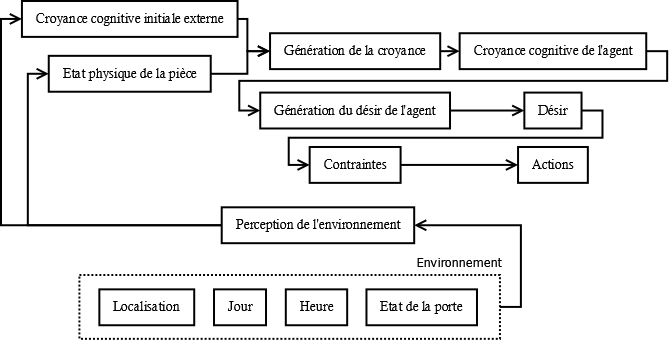
\includegraphics[scale=0.4]{Images/diagrammes_SMA/BRAHMS}
\caption{Diagramme représentant les éléments de la simulation sous BRHAMS pour la gestion de l'ouverture des portes}
\label{fig:Diagramme_BRAHMS}
\end{figure}

Malgré ce processus lourd propre à BRAHMS, Gaaloul et al. \cite{Gaaloul-12} l'ont couplé avec le logiciel COMFIE, afin de montrer l'intérêt de l'architecture à base de composant. Cette co-simulation entre COMFIE et BRAHMS est orchestrée par SIMULINK et apporte satisfaction dans les scénarios générés par BRAHMS, mais pas en terme de synchronisation et de temps de calculs. En effet, pour une simulation de 20 heures d'un bâtiment de deux zones, la durée de simulation est d'environ 20 minutes, soit plusieurs jours pour une simulation d'une année complète. 

\subsection{Repast}

Repast (\textit{REcursive Porous Agent Simulation Toolkit}) est une plateforme de modélisation et simulation avancée, gratuite et libre à base d'agents initialement développé à l'\textit{University of Chicago}. Il existe deux éditions, \textit{Repast Simphony} développé en Java, interactif et relativement facile à utiliser et \textit{Repast HPC (High-Performance Computing)} développé en C++ pour les experts qui utilisent des super-ordinateurs. Repast peut être codé sous plusieurs langages et peut intégrer des fonctions adaptatives, tels que des algorithmes génétiques, également appelés arbres de décision.

%Lacroix et al. \cite{Lacroix-12} a présenté ses travaux sur le contrôle des systèmes thermiques dans les bâtiments par gestion multi-agents. Ce projet a pour objectif d'optimiser la gestion de l'énergie en considérant l'impact économique  du prix de l'énergie. En plus de gérer la demande d'énergie, la gestion multi-agent au travers de Repast permet d'intégrer les sources d'énergies alternatives. L'architecture se base sur quatre types d'agents: des consommateurs, des producteurs, des distributeurs et des agents environnementaux. Le bâtiment est ici décrit comme un système multi-agent qui gère automatiquement les systèmes de contrôle thermique: chauffage, ventilation, air conditionné, production d'eau chaude sanitaire. Les résultats de cette étude montrent qu'un surcout de 2,5 \% entraine 35 \% de confort thermique supplémentaire.

Alfakara et Croxford \cite{Alfakara-14} utilisent Repast Simphony pour modéliser le comportement des occupants en confort estival dans les logements. Le modèle permet aux agents virtuels de Repast d'agir sur l'ouverture des fenêtres et sur l'activation de l'air conditionné. La modélisation des occupants se base sur la création d'agents: avec des propriétés individuelles (âge, style de vie, tolérance à la température, ...), autonomes et pouvant interagir entre eux. Le développement de ce modèle sous Repast permet par la suite d'étudier l'impact du comportement des occupants sur les consommations de climatisation. En effet, le SMA est couplé dynamiquement à un logiciel de simulation thermique, EDSL, qui traite le bâtiment et son environnement. Un objectif de cette étude est alors de comparer comment la manière de ce comporter vis à vis de la gestion des surchauffes modifie les consommations énergétiques. L'arbre de décision en Figure \ref{fig:Diagramme_Repast} montre le fonctionnement de Repast pour gérer les ouvertures de fenêtres et les actions sur la climatisation. Le processus décisionnel se présente alors comme un algorithme linéaire assez simple dans cet exemple, mais il peut être complexifié sans contrainte majeure. En amont de ce processus il est nécessaire de générer les agents et leurs propriétés intrinsèques.

\begin{figure}[H]
\centering
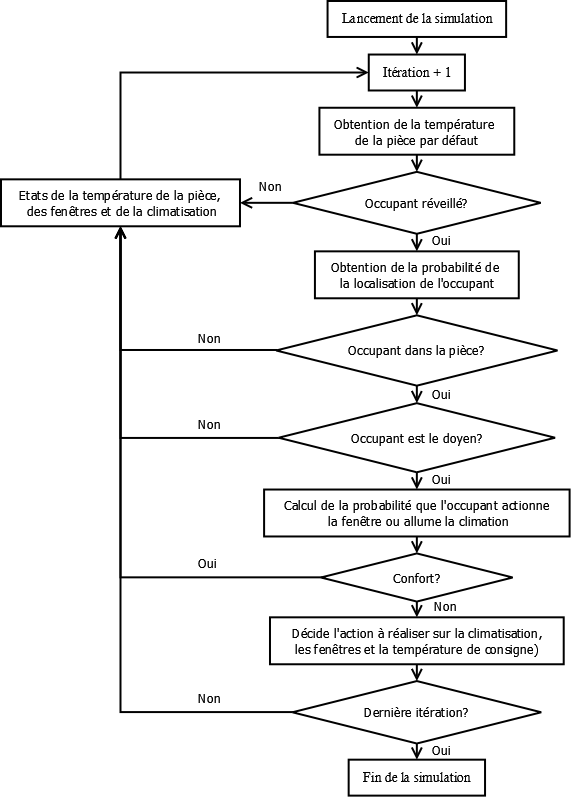
\includegraphics[scale=0.4]{Images/diagrammes_SMA/Repast}
\caption{Digramme décisionnel représentant les éléments de la simulation sous Repast pour la modélisation du confort estival}
\label{fig:Diagramme_Repast}
\end{figure}

\subsection{NetLogo}

NetLogo est une plateforme open-source SMA de modélisation de phénomènes collectifs. La plateforme est bien adaptée à la modélisation de systèmes complexes composés de centaines d'agents agissants en parallèle. La plateforme offre la possibilité de créer ses propres modèles constitués de trois types d'agents: les "\textit{turtles}" qui se déplacent dans leur environnement, les "\textit{patchs}" qui sont une portion statique de l'espace et les "\textit{observers}" qui organisent et donnent des instructions aux autres agents. NetLogo permet des modélisations des sciences sociales et naturelles de manière relativement simple.

Andrews et al. \cite{Andrews-11} ont utilisé NetLogo pour tester comment les bâtiments réagissent en fonction du comportements des occupants. Le comportement a été illustré sur l'application du confort des agents à la lumière et à son intensité. La modélisation du comportement des usagers sur la plateforme NetLogo doit pouvoir à terme être intégrée à une maquette numérique de type BIM. En effet, les limites du BIM peuvent être repoussées assez loin et une intégration des activités des occupants est à prévoir. Dans ces travaux, le lien est réalisé entre l'approche bien connue du BDI (\textit{Belief - Desire - Intension}) qui considère les croyances, les désires et les intentions des occupants et l'approche TPB (\textit{Theory of Planned Behaviour}) qui se base sur un modèle normalisé du comportement humain. L'objectif de ce couplage est alors de rendre la modélisation du comportement des occupants encore plus rationnelle que ce qui a l'habitude de se faire. La Figure \ref{fig:Diagramme_NetLogo} présente le processus décisionnel général correspondant qui mène à un comportement ou une action en utilisant la plateforme NetLogo. La modélisation dite de type \textit{BDI} est mise en évidence dans la première partie de l'algorithme puis la \textit{TPB} dans la deuxième, cela afin d'en définir l'état environnemental suivant.

\begin{figure}[H]
\centering
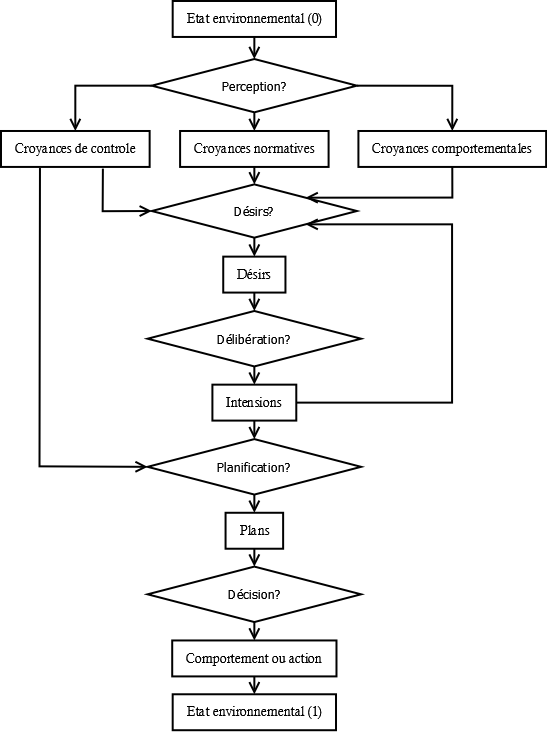
\includegraphics[scale=0.4]{Images/diagrammes_SMA/NetLogo}
\caption{Diagramme décisionnel représentant les éléments de la simulation sous NetLogo avec la combinaison \textit{BDI} et \textit{TPB}}
\label{fig:Diagramme_NetLogo}
\end{figure}

\subsection{OASys}

Cette sous-section est présentée différemment des autres puisque la plateforme OASys (\textit{Occupants’ Actions System}) fait partie de la deuxième catégorie de plateforme présenté dans ce chapitre. En effet, le développement par l'Université de Toulouse d'OASys a été codé sous JAVA pour ensuite être couplé à TRNSYS via C++. La modélisation du comportement des occupants n'utilise alors pas de plateforme pré-existante comme les travaux d'Andrews et al. \cite{Andrews-11}, d'Alfakara et Croxford \cite{Alfakara-14} ou encore de Tijani \cite{Tijani-14}.

Le cœur de la modélisation de Bonte \cite{Bonte-14} est basé sur le confort des occupants via un algorithme d'intelligence artificielle. Le modèle permet alors de prendre en compte les préférences interindividuelles et la simulation des actions des occupants en fonction de leurs sensations thermiques ou visuelles. L'unité de recherche couple par la suite la plateforme OASys avec le logiciel de Simulation Thermique Dynamique TRNSYS pour étudier l'influence du comportement des occupants sur la performance énergétique des bâtiments. La Figure \ref{fig:Diagramme_OASys} représente les éléments modélisés de la simulation sous OASys. Cela permet de bien visualiser que la modélisation de la part humaine est réalisée en deux étapes. Premièrement l'état physiologique est évalué par des modèles sur la sensation thermique et visuelle fins, et ensuite une réaction comportementale associée à une action est transmise à l'outil de STD pour en modifier l'environnement intérieur.

\begin{figure}[H]
\centering
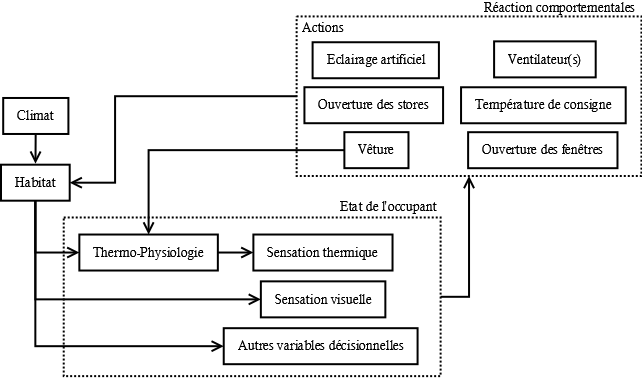
\includegraphics[scale=0.4]{Images/diagrammes_SMA/OASys}
\caption{Diagramme représentant les éléments de la simulation sous OASys avec la mise en avant de l'importance du confort}
\label{fig:Diagramme_OASys}
\end{figure}

\subsection{MASS}

Comme OASys, MASS (\textit{Multi-Agents Stochastic Simulation}) est une plateforme développée sans l'utilisation de plateforme SMA générale, mais développée sous C++ sur-mesure à la modélisation des individus dans les bâtiments. Ainsi, le développement de la plateforme et son utilisation sont réalisés au sein de la même unité de recherche.

MASS est développé par Robinson et son équipe et a pour objectif de réduire le \textit{performance gap} en mieux modélisant le caractère imprévisible des occupants. Cette plateforme développée par l'Université de Nottingham prend en compte les actions des occupants et leur nature imprévisible en couplant une modélisation stochastique avec une modélisation à base de systèmes multi-agents afin de servir le logiciel de simulation thermique EnergyPlus. Chapman et al. \cite{Chapman-14} précisent que la description de la structure (de la génération de ménages aux différents paramètres attribués à la simulation) ont une vraie utilité pour pouvoir étudier un large panel d'études de cas (résidentiel ou non résidentiel) sous différents climats. Le développement de MASS, sous C++, a été réalisé par l'utilisation de sous-modèles (activités, gains internes, ombrage, interactions entre les agents) qui sont testés par études de sensibilité pour sélectionner les plus influents et pour s'assurer que le modèle du comportement n'est pas trop lourd. La plateforme devant être lancée en 2015, il restait fin 2014, certains travaux à réaliser comme une meilleure adaptation pour le confort, l'ajout de nouveaux types de comportements, l'intégration de la modélisation de l'électricité spécifique ou encore des interactions entre les agents. Des modèles UML (\textit{Unified Modeling Language}) vont également être créés pour décrire comment les interactions fonctionnent et comment sont implémentées les règles pragmatiques dans la plateforme à base d'agents. Les règles qui auront un impact significatif sur la performance des bâtiments vont donc permettre de savoir où les futurs efforts doivent être faits pour créer de nouveaux modèles valides. La Figure \ref{fig:Diagramme_MASS} présente le diagramme décisionnel général du modèle MASS. Celui-ci nous permet de mieux visualiser les différents composants de la plateforme, c'est à dire le pré-processus, les agents et les actions associées. L'association de la plateforme au logiciel EnergyPlus permet alors une modélisation plus complète des bâtiments.

\begin{figure}[H]
\centering
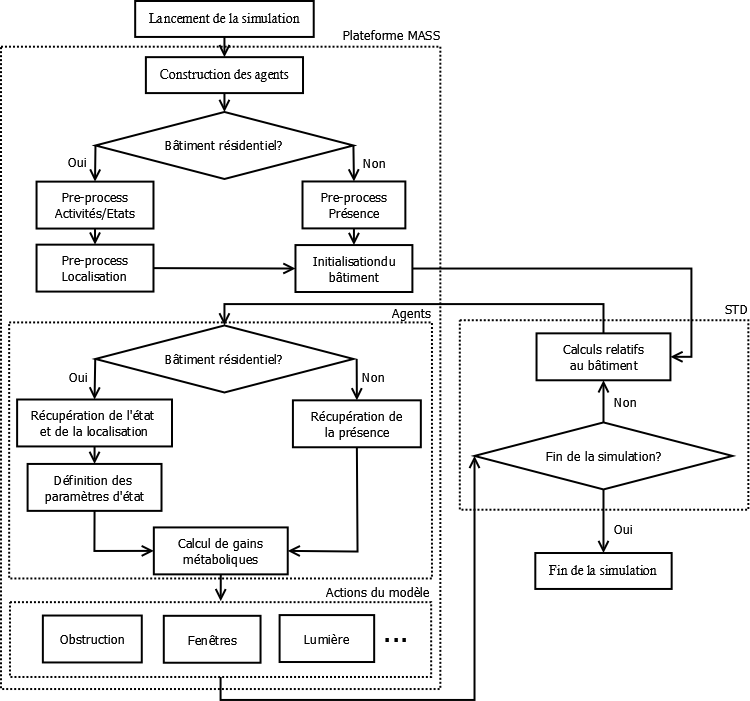
\includegraphics[scale=0.4]{Images/diagrammes_SMA/MASS}
\caption{Diagramme décisionnel représentant les éléments de la simulation sous MASS et la liaison avec EnergyPlus}
\label{fig:Diagramme_MASS}
\end{figure}

\subsection{Composant W de TRNSYS}

Bien que dans ce chapitre sur le choix de plateforme, ce paragraphe est justifié dans le sens où le composant W proposé par le logiciel TRNSYS permet de développer des composants dans un langage simple et spécialement conçu pour la simulation dynamique. Le potentiel de ce composant a été étudié pour savoir s'il pouvait recréer toutes les fonctionnalités de MASS ou d'autres modèles de comportement pour une application en bureaux d'études.

Ce composant à vil prix de 195 \euro{} \footnote{http://boutique.cstb.fr/Product/langage-w} permet une extension illimitée par bloc de TRNSYS sur une interface conviviale et sous un développement de haut niveau (langage W), c'est à dire éloigné de la machine et sans gestion de mémoire. L'utilisation du composant W simplifie le code lourd généré par l'utilisation des FMU, DLL, XML et autres scripts Python(cf chap suivant) qui servent à la co-simulation entre le logiciel de STD et la plateforme de modélisation des comportements.

En revanche, et bien que l'utilisation du composant W de TRNSYS simplifie la gestion par son approche modulaire, ce langage est bridé car il ne permet pas l'intégration de bibliothèque externe et empêche la modélisation de certains aspects comme le bouclage général de la simulation. Aussi, cela implique de re-coder en W des modèles qui existent ce qui demande un investissement en temps considérable. Enfin, le pré-processus de la simulation sous W est très difficilement géré gracieusement car il nécessite l'utilisation d'un logiciel externe, tout comme des fichiers XML avec MASS par exemple: cela n'aboutissant donc pas à la simplification d'utilisation par rapport à une co-simulation. 

Cette sous-section apparait donc ici comme un bonus aux plateformes de modélisation du comportement des occupants existants puisque seul le composant W ne permet pas le développement d'une plateforme. Il découle donc d'une réflexion sur son pouvoir de remplacer les plateformes traditionnelles utilisées en co-simulation avec les logiciels thermiques dynamique. Co-simulation qui semble en l'état ingérable pour des industriels de type bureaux d'études.

\section{Synthèse}

L'étude de la modélisation du comportement des usagers des bâtiments nous a amener à constater que par le passé plusieurs approches avaient été réalisées. Des plus simples comme les modèles basés sur des valeurs moyennes ou des scénarios déterministes au plus modernes comme les modèles à base d'agents, tous ont leurs avantages et inconvénients. Un des objectifs de la thèse étant de faire gagner aux outils de Simulation Thermique Dynamique de la fiabilité par une prise en compte plus réaliste des comportements humains, il nous a semblé logique de nous orienter vers une approche suffisamment détaillée et proche de la réalité. Le choix du type de modèle s'est alors porté d'une part vers les Systèmes Multi-Agents pour modéliser la singularité des individus mais également d'autre part à une modélisation stochastique pour modéliser la part d'aléatoire du comportement.

Les outils permettant de modéliser les comportements à base de SMA sont synthétisés dans le tableau \ref{tab:syntheseSMA}. Il permet  de révéler la diversité des approches et la maturation des projets.

\begin{table}[h]
\begin{center}
\begin{tabular}{{|p{3cm}||p{2.5cm}|p{2.5cm}|p{3.5cm}|p{3.5cm}|}}
\hline Plateforme - [Référence] & Reprise d'une plateforme générale & Outils STD & Potentiel de finesse de la modélisation & Fonctionnalité en BE \\
\hline
\hline BRAHMS - \newline Tijani et al. \cite{Tijani-14} & Oui & Pas encore couplé & Très fin - basé sur les sciences cognitives & Quasi impossible: demande un énorme travail \\
\hline Repast - \newline Alfakara et al. \cite{Alfakara-14} & Oui & EDSL 2012 & Moyen - basé sur le bon sens du modélisateur & Non - Application spécifique au confort estival \\
\hline NetLogo - \newline Andrews et al. \cite{Andrews-11} & Oui & MATLAB & Fin - basé sur les théories \textit{BDI} et \textit{TPB} & Possible - Modèle comportemental à simplifier \\
\hline OASys - \newline Bonte et al. \cite{Bonte-14} & Non & TRNSYS & Fin  - basé sur le confort thermique et visuel & Modèle comportemental à simplifier \\
\hline MASS - \newline Chapman et al. \cite{Chapman-14} & Non & EnergyPlus & Moyen - basé sur des comportements réactifs & Assez difficilement à l'heure actuelle \\
\hline Composant W & Non & TRNSYS & Grossier - L'impossibilité d'insérer des bibliothèques bride le développement & Totale \\
\hline
\end{tabular}
\caption{Synthèse des modèles à base d'agents servant à créer un lien avec un outil STD}
\label{tab:syntheseSMA}
\end{center}
\end{table}

Suite à la revue des travaux réalisés modélisant les occupants et leurs comportements par des simulations multi-agents, trois choix se sont opposés. Le premier consistait à utiliser une plateforme multi-applications pour ensuite développer les modèles comportementaux. Cette première option avait l'avantage de pouvoir développer des agents cognitifs évolués en exploitant pleinement le potentiel des SMA et de l'intelligence artificielle mais le développement fin qu'implique ces plateformes allait à l'encontre des objectifs initiaux de proposer une modélisation globale et exploitable des comportements. Le second choix était d'intégrer en cours de développement une unité de recherche. L'\textit{annex 66} a permis de rencontrer Robinson de l'Université de Nottingham, précurseur dans le domaine, avec qui une synergie a été évoquée. Cette option avait l'avantage de poursuivre et de récupérer des travaux en cours mais impliquait une mise à niveau importante principalement en terme de logique informatique d'autant plus délicate que le laboratoire partenaire était géographiquement peu accessible. La troisième option était de reprendre le fond du travail de Nottingham sous l'éditeur de composant dynamique de TRNSYS mais dans simplifier la forme. L'avantage principal à cette option était de pouvoir proposer, à terme, des composants plus modulaires et accessibles pour un bureau d'étude technique que du code primitif C++ et des fichiers xml. L'inconvénient de cette option était le manque de puissance nécessaire pour obtenir une plateforme complète, ce choix  

Le choix final c'est porté sur la collaboration avec l'université de Nottingham, la plateforme MASS (\textit{Multi-Agents Stochastic System}) et son application sont donc l'objet de la partie suivante.


\chapter{Simulation Stochastique à base d'agents (MASS)}
\label{MASS}

L'État de l'art sur la modélisation du comportement des occupants nous a donc amené à nous orienter vers une modélisation stochastique à base d'agents. Le travail réalisé n'aurait pas été possible sans l'Université de Nottingham et particulièrement son unité de recherche \textit{Building and Urban Physics and Head of the Energy and Sustainability Research Division} qui nous a fait partager son travail sans contrepartie. Avant de rentrer dans le cœur du chapitre nous tenons alors à remercier Darren Robinson et son équipe. 

Ce chapitre présente dans un premier temps l'architecture par laquelle se fait l'intégration des modèles du comportement des occupants dans les programmes de simulation énergétique puis présente dans un second temps la stratégie générale de développement de l'outil MASS.

\section{Intégration de modèles comportementaux aux logiciels de simulations thermiques dynamiques}

S'inspirer de la partie 6 du papier: "Occupant behavior modeling for building performance simulation: Current state and future challenges"  Da Yan, 2015. Puis ajouter les intérêts de la co-simulation p140 2012-Gaaloul thèse.



\section{MASS: Un Système Multi-Agents simplifié}

Nous avons proposé une définition systèmes multi-agents dans la section \ref{Systèmes Multi-Agents}. Cette définition est controversée et extrêmement large. Si on se tient à la définition la plus rigoureuse des agents par l'informaticien Ferber \cite{Ferber-95} alors MASS n'est pas un système multi-agents. En effet, selon cette définition un agent est une entité physique ou virtuelle:
\begin{itemize}
  \item qui est capable de percevoir son environnement,
  \item qui est capable d'agir dans son environnement, 
  \item qui peut communiquer directement avec d'autres agents,
  \item qui est influencé par un ensemble de tendances,
  \item qui possède des ressources propres,
  \item qui possède des compétences et offre des services,
  \item et qui peut éventuellement se reproduire, mourir et changer d'état
\end{itemize}
Or les agents de MASS n'ont ni la capacité de communiquer avec d'autres agents, ne sont pas influencés par des tendances, n'ont pas de ressources propres et ne possèdent pas de compétences particulières.

Néanmoins, dans son livre, Ferber \cite{Ferber-95} donne également la définition d'un agent réactif tropique. En opposition à un agent réactif pulsionnel qui est dirigé par des buts, l'agent réactif tropique ne répond qu'à des stimuli de l'environnement, son comportement étant guidé intégralement par l'état local du monde dans lequel il se trouve plongé. Il s'agit alors d'actions totalement réflexes sans but ni état interne. On peut alors en toute légitimité appeler les agents de MASS des agents réactifs tropiques, et son ensemble un système multi-agents réactif tropique.

\section{Architecture du modèle}

Due à leurs nature intrinsèquement différente, le comportement des occupants et celui des bâtiments sont modélisés deux différents paradigmes. Le comportement des occupants est décrit par MASS qui est une modélisation à base d'agents, alors la modélisation des bâtiments est décrit par des équations différentielles typiques des modélisations thermiques dynamiques. Une telle différence de ces systèmes complexes ne peut pas être modélisée efficacement dans un outil unique, le couplage par FMI est alors une solution. [Coupling OB with a building energy model - A FMI application, Plessis, 2014]

Interet de la dll: L'utilisation d'une bibliothèque (dll) est un excellent moyen de réutiliser le code. Au lieu d'implémenter les mêmes routines dans chaque programme que vous créez, vous les écrivez une seule fois, puis vous les référencez dans les applications qui requièrent ces fonctionnalités. En plaçant du code dans la DLL, vous économisez de l'espace dans chaque application qui la référence, et vous pouvez mettre à jour la DLL sans recompiler toutes les applications.

Ce paragraphe présente comment le FMU (Functional Mockup Unit) est implémenté pour la co-simuilation avec Energyplus. L'utilisation d'une interface externe via FMU à EnergyPlus a été réalisé pour la première fois en 2013 par le Lawrence Berkeley National Laboratory de Berkeley et présenté par Nouidui et al. \cite{Nouidui-13}. Ils ont présenté les concepts des FMI et FMU ainsi que proposé des cas d'applications sur un système CVC et sur le contrôle des stores.

....Continuer en se basant sur l'article de Nouidui \cite{Nouidui-13}.... et sur l'Annex 60

Le développement de la plateforme multi-agents est réalisé en C++, comme le montre la figure \ref{fig:CPP}, ce langage est de bas niveau, c'est à dire proche de l'assembleur de l'ordinateur. Son approche est délicate car le développeur nécessite de bien comprendre le fonctionnement de base de l'ordinateur et notamment la gestion dynamique de la mémoire. En revanche, il est très répandu donc bien documenté, il est rapide donc bien adapté pour de la co-simulation avec un logiciel externe, il est portable donc un même source code peut être transformé en exécutable Windows, MAC OS et Linux et il est surtout multi-paradigme donc son code est organisé en blocs réutilisables grâce à la programmation orientée objet (POO).

\begin{figure}[H]
\centering
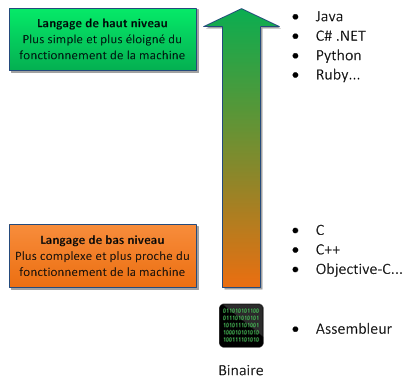
\includegraphics[scale=0.8]{Images/CPP}
\caption{Différents niveaux de langage}
\label{fig:CPP}
\end{figure}

L'idée générale du développement est de pouvoir greffer aux logiciels existant un module du comportement des occupants qui peut être utilisé de trois manières différentes. Premièrement, le modèle du comportement peut fonctionner indépendamment de l'outil de STD comme un fichier exécutable pour pré-calculer les présences et les activités. Deuxièmement, il peut être intégré au programme de simulation énergétique comme une bibliothèque dynamique, appelée en anglais \textit{Dynamic Link Library} (DLL). Troisièmement, le modèle du comportement peut-être utilisé via une co-simulation avec d'autres programmes.

D'un point de vue technique la co-simulation dynamique de MASS et d'EnergyPlus est réalisée grâce à l'outil FMI (\textit{Function Mock-up Interface)} qui utilise dans notre cas la combinaison de fichiers XML et de programmes C++. En réalité l'outil FMI nécessite un composant qui va l'implémenter, c'est le FMU (\textit{(Function Mock-up Unit)}. EnergyPlus est le co-simulateur dynamique maître car il contrôle l'échange de données et la synchronisation des programmes C++ qui composent le FMU.

Pour utiliser le FMU en co-simulation, il y a deux étapes importantes: le pré-processus et la co-simulation. L'étape de pré-processus génère une section du fichier d'entrée d'EnergyPlus (*.idf) qui peut être utilisée pour configurer le FMU pour la co-simulation. Ce fichier d'entrée définit les entrées et les sorties pour d'une part EnergyPlus mais également pour le FMU. Deuxièmement, l'étape de co-simulation exécute la simulation elle-même avec les échanges dynamiques entre EnergyPlus et le FMU.

La figure \ref{fig:FMU} montre les étapes du pré-processus pour la co-simulation via FMU.

\begin{figure}[H]
\centering
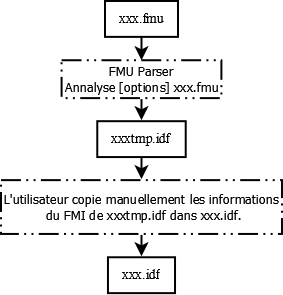
\includegraphics[scale=0.4]{Images/FMU_Pre-process}
\caption{Cheminement du pre-processus du FMU}
\label{fig:FMU}
\end{figure}

The FMI development is part of the ITEA2 MODELISAR project(2008 - 2011; 29 partners, Budget: 30 Mill. \euro). FMI development initiated, organized and headed by Daimler AG (Mercedes-Benz)

Dans MASS un agent correspond à une personne individuel et une famille correspond à un groupe d'agents.

\section{Interopérabilité des outils de MASS}

Intérêt de la co-simulation: p140 2012-Gaaloul thèse.

Comment utiliser MASS pour une co-simulation avec TRNSYS, COMFIE, ...? 2012-Gaaloul-Interopérabilité basée sur les standards Modelica et composant logiciel pour la simulation énergétique des systèmes de bâtiment

\section{Fonctionnement du FMI}

Le FMI standard compose le cœur de la co-simulation, il permet de faire l'interface entre le logiciel de simulation dynamique et la plateforme MASS. La Figure \ref{fig:diagramOfTheCo-Simulation} détail le processus et le fonctionnement.

\begin{figure}[H]
\centering
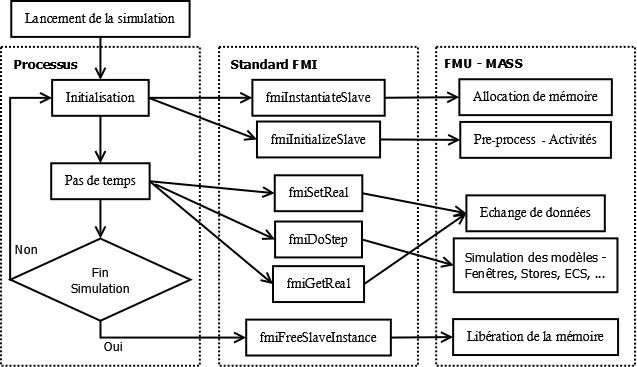
\includegraphics[scale=0.45]{Images/diagramOfTheCo-Simulation}
\caption{Diagramme de l'utilisation de l'interface de co-simulation FMI}
\label{fig:diagramOfTheCo-Simulation}
\end{figure}

\section{Stratégie générale de développement}



\section{Validation des modèles du comportement des occupants}

Le développement de modèles résulte de campagne de mesures et d'analyses. Or, une étape fondamentale est parfois négligée, il s'agit de celle de validation des modèles. La majorité des processus de validations passés sont limités à la comparaison des sorties de la simulation aux données dans le même contexte que le modèle a été développé. Cela mène à une surestimation des performances du modèle. Cette section présente les approches de validation de modèles pour le comportement des occupants.
On recense deux types de validation; les procédures de validation internes et les procédures de validation externe. Steyerberg \cite{Steyerberg-03} définit les données externes comme des données venant de mesures différentes mais venant tout de même d'une population plausiblement liée.
Dans le contexte du comportement des occupants dans les bâtiments il y a au moins trois dimensions externes à considérer: le temps, l'environnement et les occupants. La question est alors de connaître quelles dimensions doivent varier pour obtenir des données externes. Si l'objectif du modèle est de modéliser un comportement dans un bâtiment particulier alors une variation dans le temps peut être suffisante pour l'obtention de données externes. Or si l'objectif du modèle est d'être généralisé à des occupants et à des bâtiments divers alors davantage de données issus d'autres occupants et d'autres bâtiments est nécessaire.
[Revisiting validation methods of OB models - Wolf - 2015]





% Prévoir à la fin de la thèse une figure qui montre les éléments qui ont été considérés dans les modèles. En reprenant la figure 7.3: Driving forces of energy-related occupant behavior du rapport de l'annex 53: Total energy use in Building - final report
\chapter{Modélisation du comportement des occupants}
\label{Modélisation du comportement des occupants}

Ce chapitre présente dans un premier temps deux étapes nécessaires à l'intégration de modèles de comportements dans MASS et dans l'environnement de simulation. Il s'agit de la collecte de données et de sa modélisation mathématique. La présentation de deux études de cas, un bâtiment de bureau et un bâtiment résidentiel, font suite avant de présenter les modèles que nous considérons comme les plus appropriés d'une part pour améliorer la fiabilité des simulations et d'autre part d'être exploitable industriellement. 

\section{Collecte de données}

Plutôt que de poser des hypothèses non-fondées sur la manière dont les occupants se comportent, nous sommes convaincu que le meilleur moyen de proposer des modèles de comportement des occupants réalistes consiste dans un premier temps à l'observer.

Yan et al. \cite{Yan-15} ont recensé plusieurs approches de collecte de données telles que les observations non-intrusives, les études de laboratoire, les observations des comportements sous l'exécution de perturbation et les enquêtes sociologiques. Nous proposons dans cette section de présenter et expliquer l'intérêt des études sur sites, des études de laboratoires et des enquêtes.

\subsection{Suivi sur site}

% Principe
Les suivis sur site consistent à monitorer passivement les comportements des occupants ainsi que les facteurs prédisposés à expliquer ces comportements. Il s'agit généralement des variables physiques environnementales internes et externes au bâtiment étudié, ainsi que des informations relatives au temps comme l'heure de la journée, le jour de la semaine ou la saison. L'explication des comportements est parfois complétée par des études en laboratoire (Section \ref{Études de laboratoire} ou des questionnaires (Section\ref{Enquêtes}).

% Exemple d'utilisation - Presence
Ces études d'observation sont très exploitées pour comprendre les comportements humains dans un environnement quotidien. La présence et le nombre d'occupants dans une zone est un pré-requis fondamental dans l'exercice de modélisation des comportements mais la détection de présence n'est pas si simple qu'il n'y parait. Les approches fréquentes sont en outre, les détecteurs de mouvements \cite{Benezeth-11}, les capteurs de dioxyde de carbone \cite{Gruber-14} et les systèmes vidéos \cite{Fleuret-08}. Toutes ont leurs défaut: les détecteurs de mouvements ne considèrent pas l'intensité d'usage, les capteurs de CO2 sont décalés temporairement et ne fonctionnent pas si les ouvrants sont ouverts et enfin les systèmes vidéos nécessitent souvent un post-traitement lourd. 

% Exemple d'utilisation - Actions adaptatives 
Le monitoring des actions adaptatives (gestion des fenêtres, des stores, de l'éclairage, du thermostat, ...) peut également prendre différentes formes. Les observations manuelles, comme l'analyse photographique ou vidéos, peuvent théoriquement être réalisées pour l'ensemble des systèmes adaptatifs mais sont limitées par l'investissement qu'elles impliquent \cite{Rea-84}. Une méthode plus commode consiste à collecter les états des systèmes adaptatifs par voie électronique. Cette approche est particulièrement appropriée au monitoring des stores \cite{Sutter-06} et à la gestion des températures de consignes \cite{Gunay-14}. Enfin, une autre méthode précise pour déterminer l'état(ouvert ou fermé) des stores, des fenêtres ou des portes consiste à disposer des contacts de feuillure. 

% Exploitation
A la suite des campagnes de mesures, l'exploitation possible est large. Dans un premier temps, le monitoring permet d'identifier les motivations et comportements principaux. Ensuite, il permet le développement de modèles mathématiques à proprement parlé comme nous le verrons en section \ref{Formulations mathématiques}.

\subsection{Études de laboratoire}
\label{Études de laboratoire}

% Principe
L'utilisation de laboratoires pour étudier le comportement des occupants sert à approfondir les études sur site, à comprendre les comportements physiologiques et biologiques ou encore à mieux appréhender certains phénomènes dont le confort.

% Exemple d'utilisation - Actions adaptatives
Contrairement au monitoring sur site, la présence et la localisation des occupants ne peut être traité en laboratoire, car les occupants ne vivent pas dans leur environnement quotidien. Néanmoins, leurs actions adaptatives peuvent être appréhendées et les conforts thermiques et visuels étudiés plus en détail \cite{Schweiker-16}.

% Exploitation
Les bâtiments laboratoires sont donc utilisés en complément pour comprendre un phénomène bien particulier. Ce type d'étude peut donc déboucher sur la proposition de modèles mathématiques de confort. Les limitations de ces travaux, sont principalement liées à la difficulté de reproduire un environnement réaliste comme les contraintes sociales ou la non connaissance du bâtiment et de ses spécificités.

\subsection{Enquêtes}
\label{Enquêtes}

% Principe
Dans notre contexte, les questionnaires et enquêtes, comme les études en laboratoire, ont pour objectif de compléter les travaux de monitoring. Ils permettent de comprendre les motivations de certains comportements.

% Exemple d'utilisation - Actions adaptatives
L'étude des activités et donc de la localisation des individus étudiés peut-être réalisé à l'aide d'enquêtes emploi du temps. Les individus doivent par exemple noter l'enchainement de leurs activités sur une journée avec une haute sensibilité \cite{Ricroch-12}.

Les questionnaires et enquêtes peuvent également être utilisés pour comprendre les actions adaptatives. Dans ce cas, les répondants doivent généralement indiquer leur niveau actuel de confort vis à vis de l'environnement ou doivent indiquer leurs comportement dans certaines situations. Les questionnaires peuvent également être utilisés pour comparer des phénomènes biologiques, psychologiques ou sociaux.

% Exploitation
Bien que très intéressant d'un point de vu sociologique, les enquêtes peuvent se révéler biaisées si les répondants ne se rappellent pas de leurs comportements et niveau de confort ou s'ils modifient leurs réponses pour le questionnaires. En effet, des travaux montrent parfois de grandes disparités entre ce que les gens pensent faire et ce qu'ils font vraiment \cite{Gauthier-15}. 

\section{Développement de modèles}
\label{Développement de modèles}

Depuis le début des années 2000, la diffusion des modèles stochastiques puis celle des modèles à base d'agents n'a cessé de faire croître le nombre de publications traitant du comportement des occupants. La Figure \ref{fig:NbPerYear} illustre cette évolution par le recensement du nombre du nombre de publications réalisé par l'Annexe 66 de l'Agence Internationale de l'Energie. 

\begin{figure}[H]
\centering
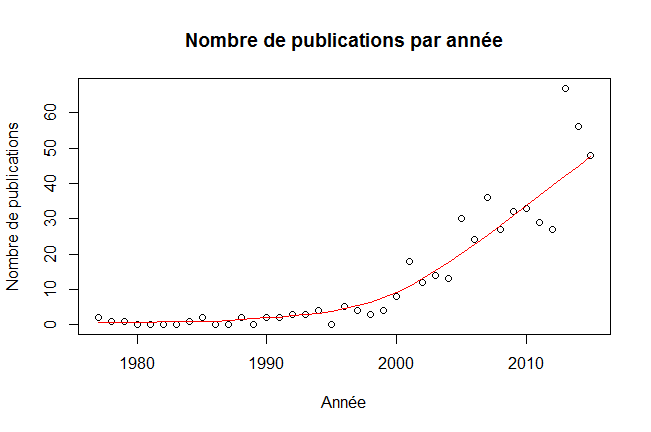
\includegraphics[scale=0.6]{Images/NbPerYear/NbPerYear}
\caption{Évolution du nombre d'articles publiés sur la modélisation du comportement des occupants}
\label{fig:NbPerYear}
\end{figure}

Le développement de modèles consiste à analyser les informations issues de la collecte et de formuler mathématiquement des lois qui en découlent. Pour rappel, un modèle permet de décrire un système en utilisant des concepts mathématiques. Il sert à prédire un état (\textit{output}) en fonction de variables explicatives (\textit{inputs}). La formulation d'un bon modèle répond à plusieurs principes: Elle est parcimonieuse, c'est à dire que les paramètres explicatifs sont statistiquement significatifs. Le modèle est basé sur des données de qualité (suffisantes, calibrées et complètes). Les outputs sont rigoureusement validés par validations croisées. Et enfin, le champ d'applicabilité est honnêtement déclaré.

Nous proposons dans cette section une revue succincte de trois formulations mathématiques fréquemment utilisées dans la modélisation du comportement des occupants, puis une présentation des méthodes d'évaluation de ces modèles.

\subsection{Formulations mathématiques}
\label{Formulations mathématiques}

Les trois formes majeures de modèles stochastiques pour représenter le comportement sont le processus de Bernoulli, les chaines de Markov et l'analyse de la survie. Le principe commun de ces formulations est de comparer une probabilité à un nombre aléatoire.

\subsubsection{Processus de Bernoulli}

Le processus de Bernoulli est un processus stochastique statique où la probabilité de l'état à prédire ne dépend pas de l'état précédent. Ce processus est une séquence de variables aléatoires indépendantes $\lbrace X_{t}:t=0,1,2,...n\rbrace$.  

$X_{t}$ est égal à 0 (l'évènement ne se produit pas) ou 1 (l'évènement se produit) pour toutes valeurs de $t$ dans le cas d'une prédiction binaire. Dans ce cas, une régression logistique binomiale est utilisée et la probabilité d'action est définit par:

\begin{equation}
P(x_{1}...x_{n}, t)=\frac{exp\left( \alpha + \sum\limits_{k=1}^n \beta_{k}x_{k}\right)}{1+exp\left( \alpha + \sum\limits_{k=1}^n \beta_{k}x_{k}\right)}
\end{equation}

avec $\alpha$ et $\beta_{k}$ l'intersection et la pente pour l'ensemble des n variables à expliquer.

Dans le cas où plus de deux résultats possibles sont à prédire, une régression logistique multinominale est utilisée, la probabilité d'action est alors définit par:

\begin{equation}
P_{j}(x, t)=\frac{exp (A_{j}(x))}{\sum\limits_{j=1}^n exp (A_{j}(x))}, j= 1, ..., N
\end{equation}
avec $A_{j}(x) = \alpha_{j} + \sum\limits_{j=1}^n \beta_{jk}x_{jk}$ et $N$ le nombre d'états.

\subsubsection{Chaine de Markov}
\label{Chaine de Markov}

Une chaîne de Markov $\lbrace X_{t}:t=0,1,2,...n\rbrace$ est un processus stochastique capable d'estimer l'état futur $X_{t+1}$ en fonction de l'état présent $X_{t}$ mais indépendamment des états passés $X_{0}, X_{1}, ..., X_{t-1}$. Elle ont l'avantage en comparaison avec le processus de Bernoulli de rendre la simulation plus fiable sur les transitions d'états. La probabilité de transition d'un état $i$ au pas de temps $t$ à un état $j$ au pas de temps $t+1$ $(T_{ij})$ peut être formulé comme:

\begin{equation}
T_{ij}(t)=P(X_{t+1}=j|X_{t}=i)
\end{equation}

On obtient alors la matrice de transition d'état $ T_{ij}(t)= \begin{bmatrix}
        T_{00}(t) & T_{01}(t) & \cdots & T_{0n}(t)\\
        T_{10}(t) & T_{11}(t) & \cdots & T_{1n}(t)\\
        \vdots & \vdots & \ddots & \vdots\\
        T_{n0}(t) & T_{n1}(t) & \cdots & T_{nn}(t)\\
     \end{bmatrix}$ pour $n+1$ états possibles.
     
Dans le cas d'un système binaire la matrice de transition $ T_{ij}(t)$ est réduite à 2 dimensions. La somme des probabilités d'une ligne étant égale à 1, il suffit de connaître deux probabilités de transition pour en déduire l'ensemble du système. La matrice réduite est donc $T_{ij}(t)= \begin{bmatrix}
        1-T_{01}(t) & T_{01}(t)\\
        1-T_{11}(t) & T_{11}(t)       
     \end{bmatrix}$

\subsubsection{Analyse de survie}

L'analyse de survie est un processus stochastique utilisé pour prédire la probabilité de durée d'un évènement. Plusieurs distributions paramétriques permettent de prédire ces durées de survie, dont la distribution de Weibull qui est la forme la plus générale. Sa densité de probabilité, ou taux de défaillance instantanée, est définit par la fonction: 
\begin{equation}
f(t) = \lambda p(\lambda t)^{p-1}e^{-(\lambda t)^{p}}
\end{equation}
avec le paramètre d'échelle $\lambda = 1/exp\left( \alpha + \sum\limits_{i=1}^k \beta_{i}x_{i} \right)$ et le paramètre de forme $log(1/p) $. Et sa fonction de survie par:
\begin{equation}
S(t) = P(T>t)=exp(-(\lambda t)^{p})
\end{equation}
A partir de la fonction de survie, lorsque l'état j commence, la durée correspondante peut être estimée en isolant $t$:
\begin{equation}
t_{j}=\frac{(-log(U))^{1/p}}{\lambda}
\end{equation}
avec $U$ un nombre aléatoire compris entre 0 et 1.

Nous pouvons noter que la distribution exponentielle peut aussi servir à l'analyse de la survie, et qu'elle est un cas particulier de la distribution de Weibull lorsque le paramètre de forme $p$ est égal à 1.

\subsection{Évaluation et validation}

Le développement de modèles résulte de campagne de mesures et d'analyses. Or, une étape fondamentale est parfois négligée, il s'agit de celle de validation des modèles. La majorité des processus de validations passés sont limités à la comparaison des sorties de la simulation aux données dans le même contexte que le modèle a été développé. Cela mène à une surestimation des performances du modèle. Cette section présente les approches de validation de modèles pour le comportement des occupants.

On recense deux types de validation; les procédures de validation internes et les procédures de validation externe. Steyerberg \cite{Steyerberg-03} définit les données externes comme des données venant de mesures différentes mais venant tout de même d'une population plausiblement liée.

Dans le contexte du comportement des occupants dans les bâtiments il y a au moins trois dimensions externes à considérer: le temps, l'environnement et les occupants. La question est alors de connaître quelles dimensions doivent varier pour obtenir des données externes. Si l'objectif du modèle est de modéliser un comportement dans un bâtiment particulier alors une variation dans le temps peut être suffisante pour l'obtention de données externes. Or si l'objectif du modèle est d'être généralisé à des occupants et à des bâtiments divers alors davantage de données issus d'autres occupants et d'autres bâtiments est nécessaire.
[Revisiting validation methods of OB models - Wolf - 2015]

\subsection{\textit{Fit-for-purpose} et facteurs contextuels}

Gaetani et al. \cite{Gaetani-16} proposent une méthodologie, appelée \textit{fit-for-purpose} permettant de sélectionner le modèle de comportement des occupants le plus approprié à l'objectif de l'utilisateur. Ce terme initialement proposé par Pitt and Myung \cite{Pitt-02} dans un contexte plus large d'analyse statistique met en garde sur la nécessité de développer des modèles qui sont ajustés aux objectifs de la modélisation. Un modèle sous-ajusté, et donc sous-paramétré, ne permet pas de reproduire le phénomène étudié, il sera alors trop rigide et ne permet pas de suivre les données. Alors qu'un modèle sur-ajusté, et donc sur-paramétré, prendra en compte des variations non-significatives et ne sera pas reproductible sur de nouvelles données. 

Yan et al. \cite{Yan-15} ont signalé dans leur article sur les futurs défis de la modélisation du comportement des occupants, que l'intégration des facteurs contextuels est un travail indispensable pour améliorer la reproductibilité des modèles. Dans la suite, nous proposons alors d'intégrer, lorsque le \textit{fit-for-purpose} n'est pas envisageable, un certain nombre de facteurs contextuels aux modèles les plus solides que nous avons préalablement identifiés.

Afin de mettre en évidence ces deux termes forts de cette thèse, la Figure de principe \ref{fig:Fit-to-purpose} met en avant la nécessité, d'une part de développer des modèles avec un niveau de complexité ni trop faible (a) ni trop élevé (c) pour obtenir des modèles parcimonieux mais néanmoins de proposer une mise en contexte des modèles afin qu'ils puissent être réutilisés pour un bâtiment autre que celui ayant servi à son développement. Ainsi, le modèle de principe utilisé dans le cadre (f) et issu du modèle (c), ne produit pas mieux les données que le modèle issu de (b) et réutilisé dans (e) malgré une qualité d'ajustement meilleure lors du développement du modèle.

\begin{figure}[H]
\centering
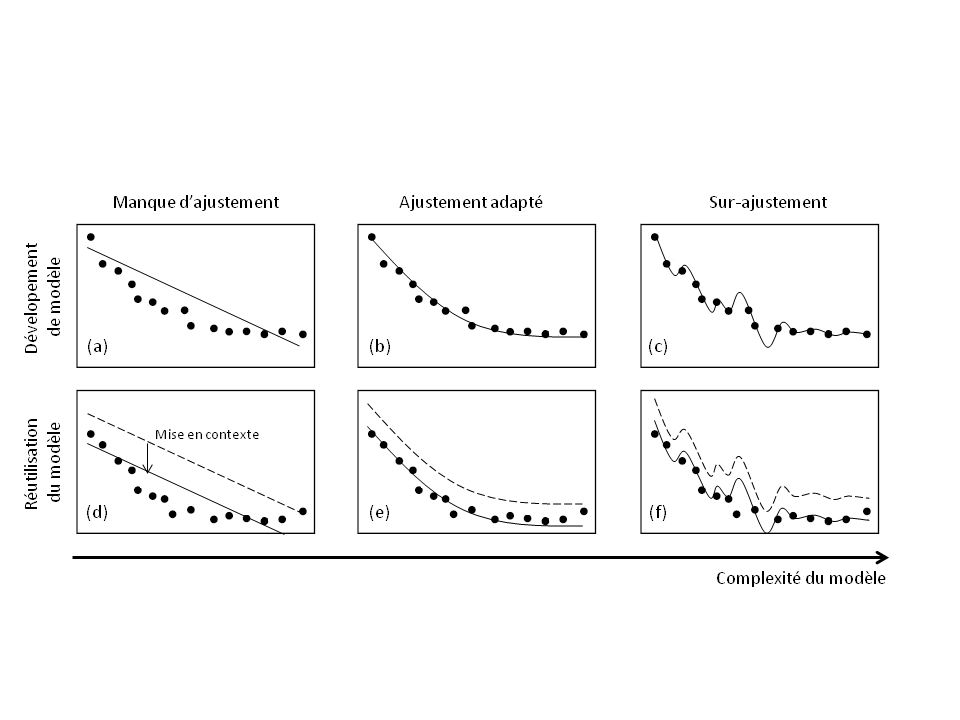
\includegraphics[scale=0.62]{Images/ComplexityAndContextualization}
\caption{Relation entre la qualité de l'ajustement (\textit{goodness of fit}), la complexité du modèle et la mise en contexte}
\label{fig:Fit-to-purpose}
\end{figure}

\section{Présentation des cas d'études}

Nous proposons dans cette section de présenter un bâtiment tertiaire virtuel et une maison individuelle conçue par l'Agence PY Architectes et notre bureau d'étude AI Environnement. Ces deux cas d'étude serviront à illustrer l'ensemble des modèles présentés plus loin dans ce chapitre. Le style architectural de ces cas d'étude est limité, en revanche les matériaux de construction sont très performants et la conception est proche d'une démarche passive.

Notre volonté initiale était de récupérer des données issues de projets réels suivi en phase d'exploitation afin de pouvoir comparer les résultats issus de nos simulations aux mesures in-situ et donc de travailler sur le \textit{performance gap}. Néanmoins, la confidentialité des documents espérés et les lenteurs administratives nous ont amené à revoir nos ambitions à la baisse. Ce changement de programme ne remet néanmoins pas en cause la co-simulation ou les modèles présentés ci-après.

\subsection{Bureau}

La Figure \ref{fig:CasEtudeBureau} représente le bâtiment de bureau, localisé en Gironde, utilisé lors des études portants sur le tertiaire. 

Par soucis de simplicité, nous avons opté pour des formes simples, nous n'avons pas intégré de masques proches ou lointains et nous avons orienté le bâtiment vers le sud. Le modèle comporte autant de zones que de pièces; 2 bureaux et un couloir. Le matériel de construction est synthétisé dans le Tableau \ref{tab:materialBureau}. Les ouvertures sont du triple vitrage argon 3/13/3/13/3 mm de coefficient de transmission thermique $U_{w}$ = 0.786 W/(m2.K). L'ensemble des ouvertures est équipé de système d'ombrage intérieur. Le renouvellement d'air est assuré par une ventilation mécanique double flux de rendement 70 \% et l'étanchéité à l'air est fixée à taux constant (pas de prise en compte météorologique) à $n_{50}$ = 0.150 Vol/h. Le bâtiment est chauffé électriquement et n'a pas de système de refroidissement actif.

\begin{figure}[H]
\centering
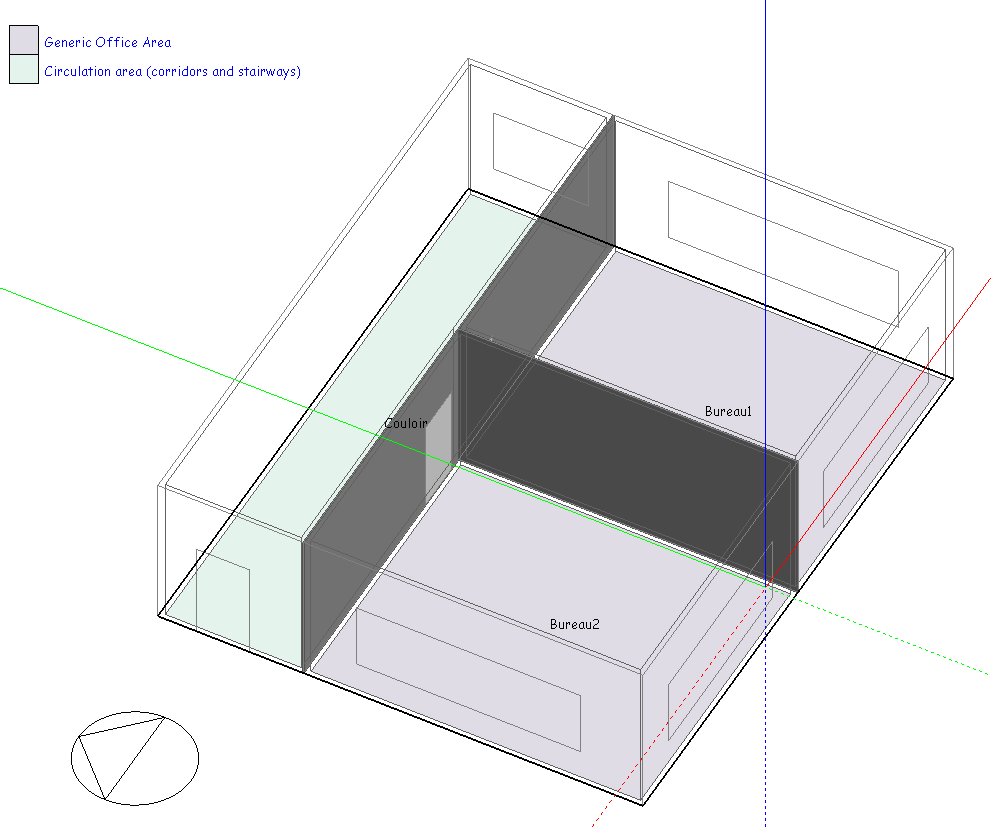
\includegraphics[scale=0.55]{Images/CasEtudeBureau}
\caption{Modèle 3D des 2 bureaux virtuels, vue du sud/ouest sous DesignBuilder}
\label{fig:CasEtudeBureau}
\end{figure}

\begin{center}
\begin{table}
\begin{tabular}{|c|c|c|c|c|}
\hline 
Construction & Couches & Épaisseur (cm) & Matériaux & U [W/(m2.K)] \\ 
\hline
\hline \multirow{3}*{Murs extérieurs} & Externe & 0.6 & Bardage métallique & \multirow{3}*{0.132} \\ 
\cline{2-4}  & 2 & 25 & Polystyrène XPS extrudé &  \\ 
\cline{2-4}  & Interne & 1.3 & Plâtre &  \\ 
\hline \multirow{4}*{Toiture} & Externe & 1 & Asphalte & \multirow{4}*{0.151} \\ 
\cline{2-4}  & 2 & 25 & Laine de verre &  \\ 
\cline{2-4} & 3 & 20 & Lame d'air &  \\ 
\cline{2-4} & Interne & 1.3 & Placoplâtre &  \\ 
\hline \multirow{2}*{Plancher} & Externe & 15 & Polystyrène XPS extrudé & \multirow{2}*{0.208} \\ 
\cline{2-4}  & Interne & 15 & Béton coulé &  \\ 
\hline \multirow{3}*{Cloisons intérieures} & Externe & 2.5 & Plaque de plâtre & \multirow{3}*{1.923} \\ 
\cline{2-4} & 2 & 10 & Lame d'air &  \\ 
\cline{2-4} & Interne & 2.5 & Plaque de plâtre &  \\ 
\hline 
\end{tabular} 
\caption{Composition et caractéristiques des matériaux de construction du bâtiment de bureau}
\label{tab:materialBureau}
\end{table}
\end{center}

\subsection{Résidentiel}

La Figure \ref{fig:CasEtudeBureau} représente la modélisation d'une maison individuelle suivant une démarche passive dans le bassin d'Arcachon à Andernos-les-Bains. Cette maison compacte est choisie comme cas d'étude pour cette thèse, car elle offre une architecture simple et performante, répondant à nos besoins de recherche. Cette compacité ne remet pas en cause les possibilités de l'outil à modéliser des cas plus complexes, mais elle a l'avantage de réduire les temps de développement et de calcul. Le découpage en zones thermiques mène à 6 zones distinctes, la buanderie ayant été intégrée au séjour et le point d'eau de la chambre ayant été transféré à la salle de bain principale (Figure \ref{fig:PlanMaison}).

Le fichier météo, issu de la base de données EnergyPlus, ayant servi à la simulation est le fichier FRA\_Bordeaux.075100\_IWEC.epw obtenu sur des mesures, sur le site de Bordeaux-Mérignac, comprises entre 1983 et 1999, suivant la procédure de création de fichiers détaillée à la section \ref{Météo}. Les caractéristiques de l'enveloppe sont présentées dans le Tableau \ref{tab:materialMaison}. Comme pour le cas de bureaux, les ouvertures sont du triple vitrage argon 3/13/3/13/3 mm de coefficient de transmission thermique $U_{w}$ = 0.786 W/(m2.K). L'ensemble des ouvertures est équipé de système d'ombrage intérieur. Le renouvellement d'air est assuré par une ventilation mécanique double flux de rendement 70 \% et l'étanchéité à l'air est fixé à taux constant (pas de prise en compte météorologique) à $n_{50}$ = 0.200 Vol/h. Le bâtiment est chauffé au gaz naturel et n'a pas de système de refroidissement actif.

\begin{figure}[H]
\centering
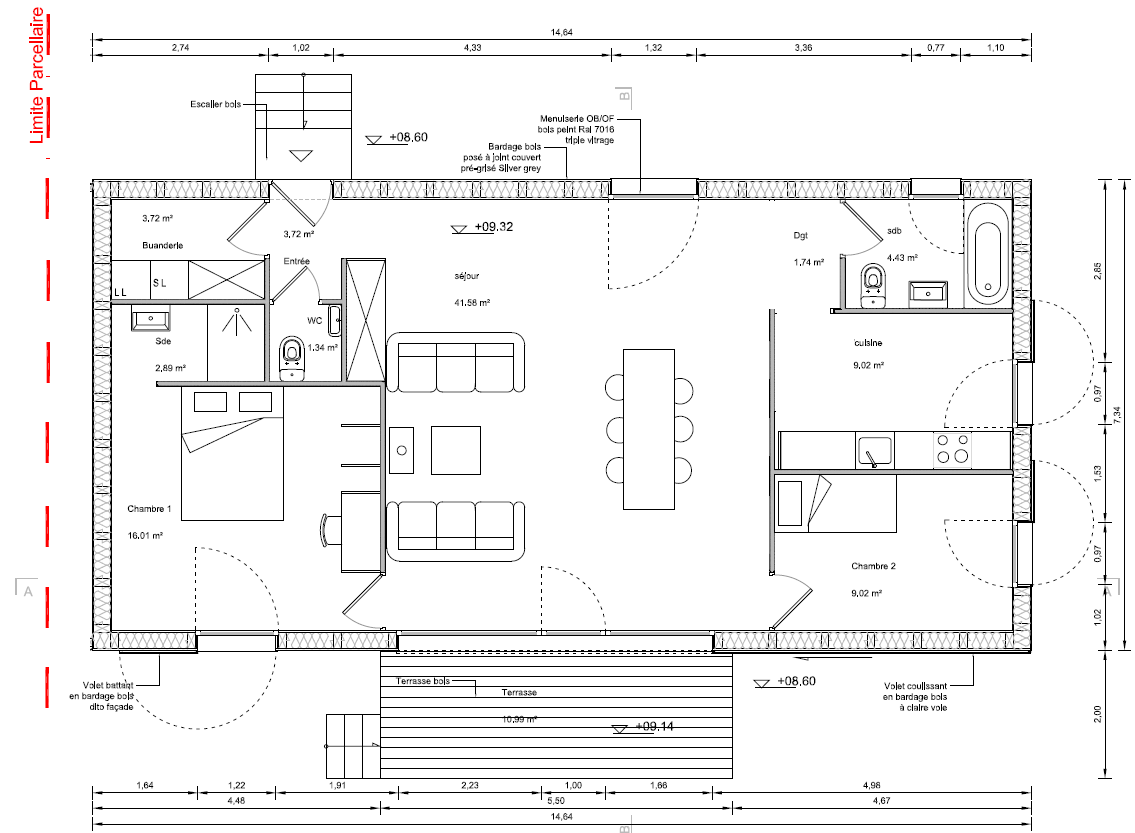
\includegraphics[scale=0.55]{Images/PlanMaison}
\caption{Plans architecte de la maison à Andernos-les-bains}
\label{fig:PlanMaison}
\end{figure}

\begin{figure}[H]
\centering
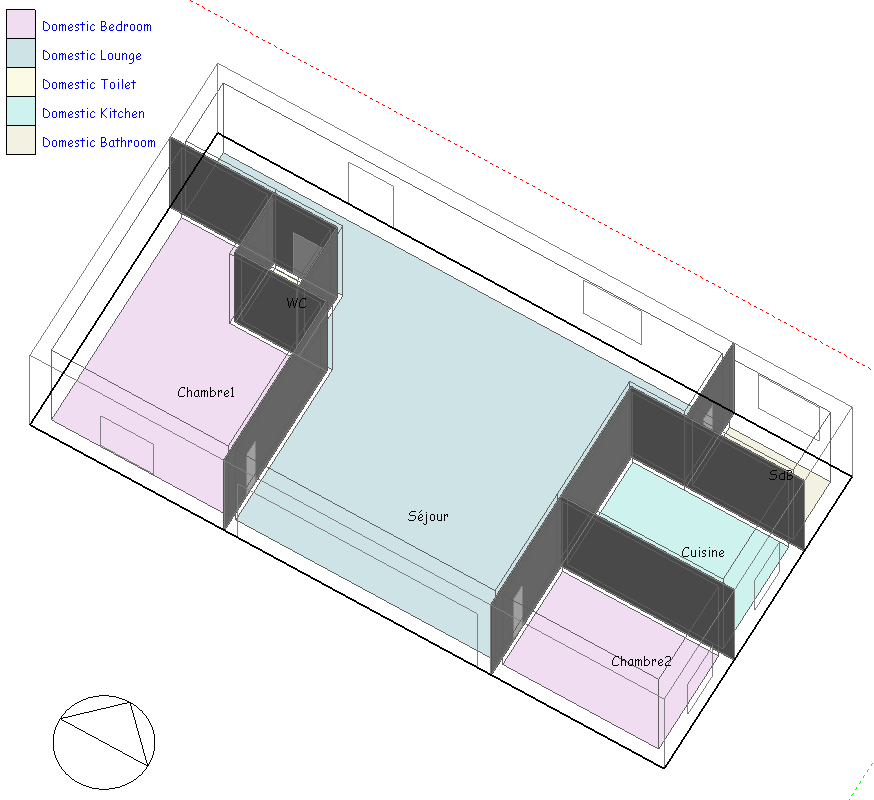
\includegraphics[scale=0.55]{Images/CasEtudeMaison}
\caption{Modèle 3D de la maison construite à Andernos, vue du sud/est sous DesignBuilder}
\label{fig:CasEtudeMaison}
\end{figure}

\begin{center}
\begin{table}
\begin{tabular}{|c|c|c|c|c|}
\hline 
Construction & Couches & Épaisseur (cm) & Matériaux & U [W/(m2.K)] \\ 
\hline
\hline \multirow{3}*{Murs extérieurs} & Externe & 1 & Enduit extérieur & \multirow{3}*{0.121} \\ 
\cline{2-4}  & 2 & 27.9 & Fibres végétales / Ossature bois &  \\ 
\cline{2-4}  & Interne & 1 & Plâtre &  \\ 
\hline \multirow{2}*{Toiture} & Externe & 35 & Panneaux de laine de verre & \multirow{2}*{0.102} \\ 
\cline{2-4} & Interne & 1 & Support métallique &  \\ 
\hline \multirow{3}*{Plancher} & Externe & 30.4 & Sol terreux & \multirow{3}*{0.376} \\ 
\cline{2-4} & 2 & 30.9 & Panneaux de laine de verre &  \\ 
\cline{2-4}  & Interne & 15 & Béton coulé &  \\ 
\hline \multirow{3}*{Cloisons intérieures} & Externe & 1.3 & Plaque de plâtre & \multirow{3}*{2.358} \\ 
\cline{2-4} & 2 & 10 & Lame d'air &  \\ 
\cline{2-4} & Interne & 1.3 & Plaque de plâtre &  \\ 
\hline 
\end{tabular} 
\caption{Composition et caractéristiques des matériaux de construction de la maison}
\label{tab:materialMaison}
\end{table}
\end{center}

\section{Présence dans les bâtiments de bureaux}

A RÉDIGER------------->: Les bâtiments accueillant des activités autres que de bureau et résidentiel, tels que les centres commerciaux, les établissement scolaires ou les musées ne sont pas modélisé car suivant des horaires de travail réguliers et spécifiques

\label{PresenceBureau}

Les scénarios de présence dans les bureaux et d'activités dans les logements constituent une entrée indispensable pour les modèles adaptatifs (gestion de température de consigne, fenêtres, stores et volets, éclairage) et non adaptatifs (utilisation d'appareils électriques, consommation d'eau chaude). Nous proposons donc dans ce chapitre et le suivant de considérer deux familles de modèles de prédiction des activités, d'une part les présences et absences dans les bâtiments de bureaux et d'autre part les activités dans les logements. Cette distinction fondamentale également partagée par plusieurs chercheurs \cite{Vorger-14}, \cite{Page-08}, \cite{Chapman-14} peut être vue comme un \textit{fit-for-purpose} dans le sens ou les modèles sont radicalement différents et n'ont pas de racines communes.

Bien que les horaires de travail et les horaires d'occupation des logements soient très corrélés pour l'ensemble de la population, les deux modèles présentés dans ce chapitre et dans le chapitre \ref{ActivitésLogements} sont totalement indépendant. Nous justifions ce choix par une modélisation dans cette thèse à l'échelle du bâtiment. Une modélisation plus large à l'échelle du quartier ou de la ville impliquerait alors une approche ou les activités professionnelles et privées seraient dépendantes.

L'objectif de ce chapitre est de proposer un modèle qui reproduit plus fidèlement la présence de travailleurs de bureaux que les scénarios conventionnels couramment utilisés. Le modèle proposé dans ce chapitre est définit en pré-processus de la simulation, c'est à dire qu'il est connu pour l'ensemble de la simulation avant que celle-ci n'ai débutée. Ce choix se justifie par la non-nécessité, à priori, de connaître les variables environnementales pour définir les horaires de travail. La première partie de cette section présente un état de l'art des modèles stochastiques de présence dans les bureaux et plus particulièrement le modèle de Page et al. \cite{Page-08} qui est utilisé comme base dans la suite. La seconde partie présente comment ce modèle développé sur des bureaux universitaires de chercheurs peut être également appliqué sur des bureaux privés. Enfin, une présentation des résultats de ce modèle et de ces sous-modèles est proposée.

\subsection{État de l'art}

Afin d'établir des modèles stochastiques réalistes de présence dans les bureaux pour associer une présence à des apports métaboliques et à des actions possibles plusieurs travaux ont été réalisés. Le Tableau \ref{tab:PresencePresentation} et \ref{tab:PresenceOffice} présentent respectivement le contexte du développement des modèles et leurs variables d'entrée et de sortie. Nous présentons avant cela les modèles les plus pertinents. 

En 1995, Newsham et al. \cite{Newsham-95} ont proposé un premier modèle probabiliste de présence simple afin de créer des scénarios d'occupation dans le cadre du travail de modélisation de la gestion de l'éclairage artificielle, lightswich. En 2003, Yamagushi et al. \cite{Yamaguchi-03} ont également développé un modèle de présence simple grave à des chaines de Markov, servant d'entrée à la prédiction de la demande d'énergie à l'échelle d'un quartier. Ces deux modèles étant très simplifiés ils ne seront pas présentés plus en détails dans les tableaux suivant.

Wang et al. \cite{Wang-05} ont examiné les propriétés statistiques d'occupation dans des bureaux individuellement occupés. Ils ont réalisé l'hypothèse que les durées des périodes de présences et d'absences intermédiaires sont distribuées exponentiellement et que le coefficient de la distribution peut être traité comme une constante sur la journée. Aussi, ils proposent de générer les premières arrivées, les premiers départs et les pauses déjeuners en assumant que ces périodes suivent une loi normale. Bien qu'élégant, ce modèle ne permet de reproduire la complexité de de présence réelle et sur-estiment la présence, tout comme les scénarios conventionnels.

Page et al. \cite{Page-08} proposent un modèle basé sur des chaines de Markov à deux états à partir d'une campagne de mesure longue sur 5 bureaux universitaire à Lausanne. Ce modèle est capable de reproduire les caractéristiques d'occupations, comme les arrivées, les départs, les absences intermédiaires et les absences longues, mais il n'est pas capable de simuler les mouvements entre les zones. Néanmoins, ce modèle est très probablement celui qui a été le plus repris dans des travaux postérieurs, notamment par Liao et al. \cite{Liao-11}, Vorger \cite{Vorger-14} et Feng et al. \cite{Feng-15}, avec de bonnes capacités de prédiction.

Erickson et al. \cite{Erickson-09} ont utilisé les données collectées d'occupation de bureaux pour développer un modèle basé sur des lois Gaussienne multidimensionnelles aux périodes de transitions. Ce modèle a par la suite été intégré dans un modèle à base d'agents dans le but de prédire la mobilité sur plusieurs zones des agents. Cependant, les résultats montrent une faible reproduction des mesures, de l'ordre de 20 \%.

Tabak et de Vries \cite{Tabak-10} ont généré des profils d'occupation basés sur l'enchainement chronologique des activités des occupants. Cette approche détaillée reproduit bien la complexité du comportement des occupants mais nécessite un gros travail de questionnaires et de mesures. Cette méthode indirecte est plus complexe à intégrer dans un outil de simulation que les autres approches mentionnées précédemment.

Davis et Nutter \cite{Davis-10} ont instrumenté 6 type de bâtiments universitaire aux activités différentes afin de proposer des profils de présence hebdomadaire selon ces familles d'activités. Les résultats synthétisent les probabilités de présence par type de bâtiment et il a été conclu que les jours de la semaines sont parfois significativement différents.

Liao et al. \cite{Liao-11} proposent un modèle permettant de suivre la location des occupants dans l'espace et dans le temps. Ce modèle puissant permet une bonne prédiction de l'occupation dans le cas de faible nombre de zone mais une prédiction approximative dans le cas de multi-zones. Les auteurs indiquent que la configuration du modèle est très chronophage et difficilement extensible.

Wang et al. \cite{Wang-11} utilisent une modélisation de la présence dans les bâtiments de bureaux basée sur les chaines de Markov à niveaux multiples. Le nombre de niveaux correspond au nombre de zones où l'agent est susceptible de se trouver. Ces travaux sont bien documentés mais relèvent plus d'une méthodologie qu'une proposition de modèle calibré, car les résultats ne sont pas issus de campagne de mesures ou d'enquêtes.

Duarte et al. \cite{Duarte-13} ont collecté réalisé une campagne longitudinale pour montrer les variations des facteurs d'occupation dans des bâtiments de bureaux selon l'heure de la journée, le jour de la semaine et le mois de l'année. Les comparaisons ont montré une variabilité élevée entre ces paramètres et un écart de la moyenne de 46 \% inférieur au standard américain ASHRAE 90.1. Ce travail met également en avant la variabilité des profils de présence en fonction des vacances et du type d'espace, notamment entre les bureaux privés et les bureaux partagés.

Chang et Hong \cite{Chang-14} ont analysé 200 bureaux cubiques de 3 étages aux activités différentes d'un bâtiment commercial. Un modèle mathématique est proposé afin de décrire le nombre et la durée des périodes d'absences. Une première fonction de densité cumulée (\textit{CDF}) définit le nombre d'absence, une seconde fonction de densité cumulée définit la durée et une distribution de probabilité (\textit{PDF}) définit le début d'une période d'absence. Les auteurs ont identifié des profils d'occupation groupés en 5 catégories prouvant la variabilité de présence.

Feng et al. \cite{Feng-15} ont développé un modèle d'occupation inspiré du modèle de Wang et al. \cite{Wang-11} qu'ils ont couplé à un logiciel de simulation thermique. Ce modèle est une chaine de Markov à 12 niveaux correspondant aux 12 zones du cas d'étude. Quelques hypothèses sont présentées dans l'article concernant les activités des différents membres du bâtiment. Il est ainsi avancé que les managers sont moins présent dans les bureaux que les chercheurs pour assister à des conférences ou participer à des réunions, cela menant à une présence dans leurs propres bureaux moins importante.

Mahdavi et Tahmasebi \cite{Mahdavi-15} ont testé 3 modèles d'occupation sur des données issues de mesures sur une Université de Vienne. Les deux premiers modèles d'occupation sont stochastiques, il s'agit du modèle proposé par Reinhart \cite{Reinhart-01} (non-détaillé ici) et celui de Page et al. \cite{Page-08}. Le troisième modèle est un modèle non-probabiliste d'apprentissage qui génère des profils d'occupation binaire journalière basés sur les données de présence passées. Une fois la phase d'apprentissage suffisamment robuste, la phase d'évaluation montre que le modèle non-stochastique prédit mieux la présence que les modèles stochastiques.

\begin{landscape}
\begin{table} [H]
\begin{tabular}{|p{2.5cm}|p{2cm}|p{2cm}|p{2cm}|p{2cm}|p{2cm}|p{4cm}|p{4cm}|}
\hline 
Auteurs & Location & Bâtiment & Durée campagne & Intervalle de mesure & Modèle & Points forts & Points faibles \\ 
\hline 
\hline
Wang et al. \cite{Wang-05}, 2005 & USA & 35 bureaux & 1 année & 15 minutes & Processus de Poisson & Présence intermédiaire modélisé; Simplicité du modèle & Bureau unique \\ 
\hline 
Page et al. \cite{Page-08}, 2008 & Suisse & 20 zones universitaires (10 bureaux) & 2 années & 15 minutes & Chaine de Markov & Détaillé pour implémentation; comparé postérieurement & Données d'entrée complexes; Sous-estimation du nombre de jour d'absence total \\ 
\hline 
Ericksen et al. \cite{Erickson-09}, 2009 & USA & 4 zones universitaires & 2 fois 1 jour & Vidéo & Multivarié Gaussien & Comparaison de modèles sur différentes zones & Durée de la campagne; Erreur des modèles importante  \\ 
\hline 
Tabak et de Vries \cite{Tabak-10}, 2010 & Pays-bas & 1 bureau (8 occupants enquêtés) & - & - & S-curve; Méthode probabiliste & Prédiction d'activités intermédiaires  & Modèle basé sur des questionnaires uniquement \\ 
\hline 
Davis et Nutter \cite{Davis-10}, 2010 & USA & 11 bâtiments universitaires & 5 mois & Vidéo & - & Identification de facteurs par type de bâtiment & Pas de modèle proposé \\ 
\hline 
Liao et al. \cite{Liao-11}, 2011 & USA & Bâtiment commercial & - & 15 minutes & Chaine de Markov & Comparaison de modèle & Campagne de mesure très peu présenté \\ 
\hline 
Wang et al. \cite{Wang-11}, 2011 & - & 5 bureaux & - & 5 minutes & Chaine de Markov à 7 niveaux & Suivi zone par zone des occupants & Modèle non-basé sur des mesures \\ 
\hline 
Duarte et al. \cite{Duarte-13}, 2013 & USA & Bâtiment commercial & 2 années & 1 minute & Modèle déterministe & Large campagne de mesures reflétant l'influence de facteurs contextuels & Pas de modèle clairement proposé \\ 
\hline 
Chang et Hong \cite{Chang-14}, 2014 & Taiwan (?) & 200 bureaux & 6 mois & 5 minutes & Fonction de distribution cumulative et de probabilité & Groupement suivant 5 familles de profils & Modèle applicable à des bureaux non-partagés \\ 
\hline 
Feng et al. \cite{Feng-15}, 2015 & - & 12 zones universitaires & - & - & Chaine de Markov à 12 niveaux  & Suivi zone par zone des occupants & Modèle non-basé sur des mesures \\ 
\hline 
Mahdavi et Tahmasebi \cite{Mahdavi-15}, 2015 & Autriche & 8 zones universitaires & 9 mois & 15 minutes & Modèle d'apprentissage & Comparaison de modèles & Profil d'occupation unique \\ 
\hline 
\end{tabular}
\caption{Synthèse des modèles les plus pertinents de présence et d'activités dans les bureaux}
\label{tab:PresencePresentation}
\end{table}
\end{landscape}

\begin{table} [H]
\centering
\begin{tabular}{|l||c|c|c|c|c|c|c|c|c|c|c|}
\hline
\textbf{Variables\textbackslash Auteurs} & \cite{Wang-05} & \cite{Page-08} & \cite{Erickson-09} & \cite{Tabak-10} & \cite{Davis-10} & \cite{Liao-11} & \cite{Wang-11} & \cite{Duarte-13} & \cite{Chang-14} & \cite{Feng-15} & \cite{Mahdavi-15} \\
\hline
\hline \rowcolor{gray}\textbf{Environnementales} & \multicolumn{11}{c}{} \\
\hline Mois/Saison &  &  &  &  &  &  &  & X &  &  &   \\
\hline Météo & / &  &  &  &  &  &  & / & / &  &   \\
\hline \rowcolor{gray}\textbf{Contextuelles} & \multicolumn{11}{c}{} \\
\hline Heure de la journée & X & X & X & X & X & X & X & X & X & X & X \\
\hline Type d'activité &  &  &  & X & X & X & X &  & X & X &  \\
\hline Jour de la semaine &  & X &  & X & X & X &  & X &  &  &   \\
\hline Activités intermédiaires &  &  &  & X &  & / & X &  &  &  &   \\
\hline \rowcolor{gray}\textbf{Bâtiment} & \multicolumn{11}{c}{} \\
\hline Type de zones &  &  & X &  & X &  & X & X &  & X &   \\
\hline \rowcolor{gray}\textbf{A expliquer} & \multicolumn{11}{c}{} \\
\hline Statut d'occupation & X &  &  &  &  &  &  &  & X &  &   \\
\hline Nombre d'occupant par zone &  & X &  &  & X &  &  & X &  &  & X  \\
\hline Location des occupants &  &  & X & X &  & X & X &  &  & X &   \\
\hline
\end{tabular}
\caption{Synthèse des données d'entrée et de sortie des modèles de présence et activités dans les bureaux}
\label{tab:PresenceOffice} 
\end{table}

Conclusions/Discussion/Choix du modèle:
\begin{itemize}
\item
\item Certains modèles permettent de prendre en compte les déplacements entre plusieurs zones du bâtiment. Toujours constitués de chaines de Markov le modèle gagne en réalisme mais s'en trouve alourdi. De plus, il est alors nécessaire de donner en entrée du modèle la probabilité de présence de chaque occupant, dans chaque zone et à chaque pas de temps
\end{itemize}

\subsection{Modèle de Page}

----
Le modèle initial ayant été développé dans un contexte universitaire, il n'est à priori pas nécessairement valide pour des bâtiment de bureaux abritant d'autres activités, les horaires de travail dépendant des catégorie socio-professionnelles. Une solution consiste à répliquer le travail de Page et al. \cite{Page-08} pour plusieurs typologies de bâtiments afin de calibrer le modèle de base. Un ajustement contextuel plus fin serait ensuite possible afin de considérer davantage de facteurs influents. Dans la suite, nous utiliserons uniquement le modèle de Page comme base ajustable, car ce modèle est le plus robuste de notre base bibliographique et en développer davantage reste un travail coûteux et chronophage. Néanmoins, afin de rendre ce modèle applicable à une gamme de bâtiments et un type d'occupants plus large, nous proposons d'y ajouter des facteurs contextuels rendant l'ensemble plus flexible et plus approprié.
----


Comme nous venons de le voir, les chaînes de Markov permettent de reproduire des transitions d'états et donc de rendre la dynamique de simulation plus cohérente avec les présences et absences des occupants. La section \ref{Chaine de Markov} a présenté le fonctionnement de base des chaînes de Markov. Page et al. \cite{Page-08} ont proposé un modèle de transition d'état pour les bâtiments de type bureau utilisant des chaînes de Markov. Sur la base de mesures de présence dans 5 bureaux de l'Ecole Polytechnique Fédérale de Lausanne pendant 4 ans, Page et al. ont proposé des probabilités de présence heure par heure pour une semaine type, soit 168 (24*7) probabilités. 

Les probabilités de transitions $T_{ij}(t)$ sont calculés à partir des probabilités de présence et l'équation suivante en est déduite:

\begin{equation}
T_{11}(t)=\dfrac{P(t)-1}{P(t)}T_{01}(t)+\dfrac{P(t+1)}{P(t)}
\label{T110}
\end{equation}

Néanmoins, une information est manquante pour déterminer les valeurs $T_{01}$ et $T_{11}$ à chaque pas de temps. Les auteurs ont alors défini un paramètre de mobilité:

\begin{equation}
\mu(t)=\dfrac{T_{01}(t)+T_{10}(t)}{T_{00}(t)+T_{11}(t)}
\label{mu}
\end{equation}

Pour simplifier les entrées du modèle et le calibrer, les auteurs ont fixé ce paramètre de mobilité ($\mu$) à 0.11. Cette valeur correspond à la valeur moyenne observée du paramètre de mobilité. Nous pouvons noter que plus $\mu$ est grand plus la transition d'état est fréquente.
A partir des équations \eqref{T110} et \eqref{mu} on peut alors déterminer les quatre probabilités de transition pour chaque pas de temps:

\begin{itemize}
\item $T_{01}(t)=\dfrac{\mu-1}{\mu+1}P(t)+P(t+1)$
\item $T_{00}(t)=1-T_{01}(t)$
\item $T_{11}(t)=\dfrac{P(t)-1}{P(t)}\left[\dfrac{\mu-1}{\mu+1}P(t)+P(t+1)\right]+\dfrac{P(t+1)}{P(t)}$
\item $T_{10}(t)=1-T_{11}(t)$
\end{itemize}

Il est à noter que pour certaines conditions, lorsque les probabilités de présence entre deux pas de temps $P(t)$ et $P(t+1)$ sont très différentes, la probabilité de transition $T_{ij}$ puisse ne pas être comprise entre 0 et 1. Dans ce cas, le paramètre de mobilité est modifié de tel façon à ce qu'il permettent à la probabilité de transition de prendre une valeur cohérente.

Lors du pré-processus de la simulation, la présence est calculés à partir des équations ci-dessus, afin d'être utilisée lors de la simulation. Pour ce faire, à chaque pas de temps un nombre aléatoire $rand$ compris entre 0 et 1 est généré par une loi uniforme, puis comparé à la probabilité de transition $T_{01}(t)$ si l'occupant est absent et à $T_{11}(t)$ si l'occupant est présent. Si $rand < T_{01}(t)$ alors l'occupant rentre dans la pièce, sinon non, et si $rand < 1-T_{11}(t)$ alors l'occupant sort dans la pièce, sinon il y reste.

Le Tableau \ref{tab:PPage} présente les probabilités de présence $P$, pour les lundis et pour les samedis, issues des mesures sur les 5 bureaux du modèle de Page et al. \cite{Page-08}. Les probabilités de présence du lundi sont représentatives de celles des jours de travail (lundi à vendredi), alors que les probabilités du samedi sont semblables à celles du dimanche. Les sorties du modèle de base sont présentés dans la section \ref{Facteurs contextuels} avec les variantes.

\begin{table}[H]
\centering
\begin{tabular}{|c|c|c|c|c|c|c|c|c|c|c|c|}
\hline 
Heure & 1 & 2 & 3 & 4 & 5 & 6 & 7 & 8 & 9 & 10  \\ 
\hline 
$P_{Lundi}$ & 0.021 & 0.021 & 0.021 & 0.021 & 0.021 & 0.021 & 0.021 & 0.025 & 0.250 & 0.422  \\ 
\hline 
$P_{Samedi}$ & 0.028 & 0.030 & 0.029 & 0.029 & 0.030 & 0.029 & 0.029 & 0.030 & 0.030 & 0.030  \\ 
\hline
\hline
Heure & 11 & 12 & 13 & 14 & 15 & 16 & 17 & 18 & 19 & 20 \\ 
\hline 
$P_{Lundi}$ & 0.309 & 0.377 & 0.187 & 0.375 & 0.426 & 0.396 & 0.375 & 0.432 & 0.084 & 0.070 \\ 
\hline 
$P_{Samedi}$ & 0.035 & 0.037 & 0.030 & 0.032 & 0.041 & 0.045 & 0.042 & 0.034 & 0.035 & 0.032 \\ 
\hline 
\hline
Heure & 21 & 22 & 23 & 24 & \cellcolor{lightgray}& \cellcolor{lightgray}& \cellcolor{lightgray}& \cellcolor{lightgray}& \cellcolor{lightgray}& \cellcolor{lightgray}\\ 
\hline 
$P_{Lundi}$ & 0.047 & 0.039 & 0.038 & 0.038 & \cellcolor{lightgray} &\cellcolor{lightgray} &\cellcolor{lightgray} &\cellcolor{lightgray} &\cellcolor{lightgray} & \cellcolor{lightgray}\\ 
\hline 
$P_{Samedi}$ & 0.027 & 0.024 & 0.021 & 0.021 &\cellcolor{lightgray} &\cellcolor{lightgray} &\cellcolor{lightgray} & \cellcolor{lightgray}&\cellcolor{lightgray} &\cellcolor{lightgray} \\
\hline 
\end{tabular}
\caption{Probabilités de présence dans les bureaux pour les lundis et les samedis}
\label{tab:PPage}
\end{table}

\subsection{Ajustement du modèle de Page et al.}
\label{AjustementPage}

Une fois le modèle brut de Page et al. \cite{Page-08} reprit dans la plateforme MASS, nous comparons nos résultats issus d'une simulation d'un an, d'un occupant et au pas de temps de 5 minutes avec ceux des auteurs pour vérifier la bonne programmation. Plusieurs observations nous amènent à proposer un ajustement du modèle de base. Celles-ci sont de deux types, d'une part les observations communes entre les codes, mais en contradiction avec nos connaissances socioprofessionnelles. Et d'autre part, des différences suffisamment significatives, entre la base et le modèle codé dans MASS, pour être rapportées ici.

La comparaison des profils de probabilités de présence est un premier bon indicateur de la qualité du modèle, la Figure \ref{fig:ProfilPresence} permet de constater une bonne reproduction globale, mais une présence semble t-il légèrement plus élevée les nuits dans notre cas. La Figure \ref{fig:ChronogrammeBase} est un chronogramme sur une année de simulation, les zones noires représentent les périodes travaillées et les zones grises les absences. Nous identifions clairement les matins et les après-midis comme périodes principalement travaillées, mais nous pouvons surtout noter des présences régulières courtes les nuits et confirmer notre impression issue du profil de présence.

\begin{figure}[H]
\centering
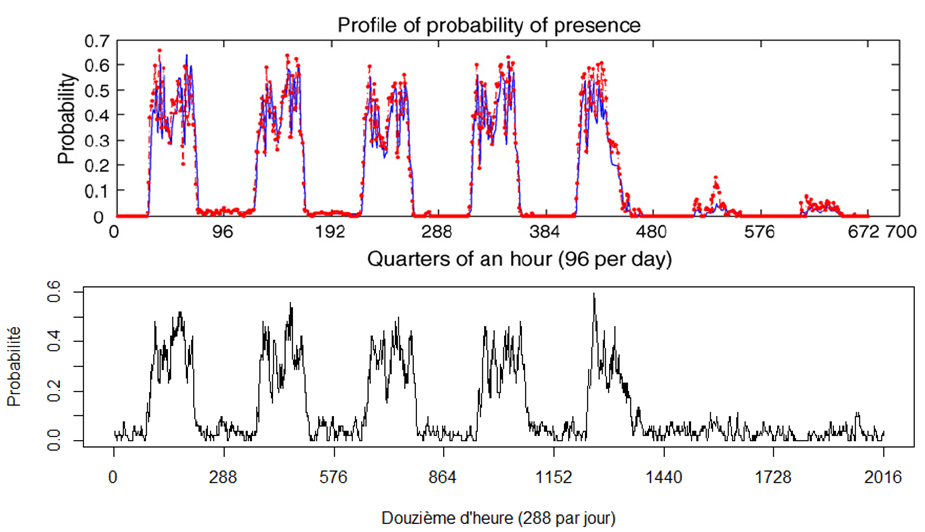
\includegraphics[scale=0.6]{Images/PageActivities/ProfilPresence}
\caption{Profils de présence mesuré (bleu) et simulé (rouge) issus de l'article de Page et al \cite{Page-08} (en haut) et généré dans la plateforme MASS (en bas)}
\label{fig:ProfilPresence}
\end{figure}

\begin{figure}[H]
\centering
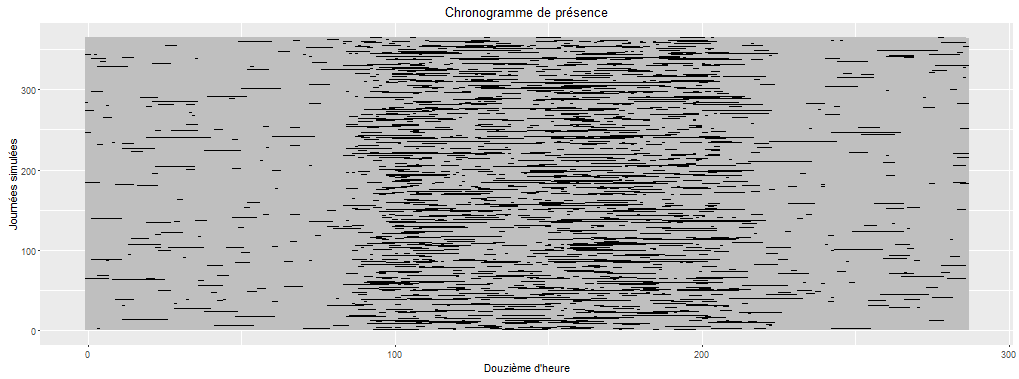
\includegraphics[scale=0.46]{Images/PageActivities/ChronogrammeBase}
\caption{Chronogramme de présence d'un agent sur un an selon le modèle initial de Page et al \cite{Page-08}}
\label{fig:ChronogrammeBase}
\end{figure}

Le second indicateur exploitable est la durée de présence dans les locaux. Dans l'article de Page et al. \cite{Page-08} une incohérence semble apparaitre. En effet, la durée de présence hebdomadaire moyenne est donnée à 24 heures soit 4h48 par jour, alors que la durée de présence quotidienne est quant à elle aux alentours de 9h par jour si l'on se fie aux graphiques. Sur une base de 5 jours de travail nous aboutissons dons à un décalage d'un facteur proche de 2. De notre côté, notre simulation nous amène à une durée moyenne de 3h49 et un écart-type de 1h24 sur les 5 jours travaillés, soit 1h de moins que la durée hebdomadaire du modèle de base.

Trois indicateurs complémentaires sont utilisés pour évaluer le modèle: l'heure de première arrivée, l'heure de dernier départ et le nombre de transitions d'états. Sur la base d'une simulation d'une année la moyenne d'heure de première arrivée est à 6h51, la médiane à 7h25 et l'écart type de 4h16, contre une médiane à 7h30 dans \cite{Page-08}. Ces résultats se justifient par la haute fréquence de présence de nuit déjà discuté en début de paragraphe. La moyenne d'heure de dernier départ est quant à elle à 17h58, la médiane à 17h50 et l'écart type de 3h56, contre une moyenne de 17h30 dans \cite{Page-08}. Le nombre moyen de transitions quotidien par jour à priori travaillé est de 12.60 et en semaine, week-end compris de 9.97, contre 8 dans \cite{Page-08}.

L'étude du modèle de base nous amène à deux remarques. D'une part le modèle produit une présence dans les bureaux trop importante les nuits et d'autre part la présence moyenne est sous-estimée par le modèle. Pour palier à ces remarques nous proposons de borner arbitrairement le modèle entre 5h et 21h, car nous estimons une présence à l'extérieure de ces bornes comme irréaliste pour un travail de bureau. De plus, afin de se caler sur les durées moyennes de travail hebdomadaire recensés par les organisations nationales de l'OECD\footnote{L'Organisation de Coopération et de Développement Économique est une organisation internationales d'études économiques - Site internet \url{http://www.oecd.org/fr/}} \cite{OECD-14} et de la DARES\footnote{La Direction de l'Animation de la Recherche, des Etudes et des Statistiques} \cite{Pak-13} qui sont données respectivement à 36h17 (2014) et 36h36 (2013), nous ajoutons un coefficient aux probabilités de présence $P(t)$. La durée moyenne de travail hebdomadaire issue de notre simulation étant de 20h31 nous pourrions proposer un coefficient de $(36h26/20h31=36.43/20.52=)1.78 $. Or, les durées issues du modèle correspondent à une présence effective dans les bureaux, contrairement aux durées tirées des études statistiques  qui sont des durées travaillées au bureau, mais également en déplacement, en réunion ou en télétravail, nous utiliserons dans la suite un ajustement des coefficients de présence abaissé à $1.7$ du lundi au vendredi de 5h à 21h. Les résultats du modèle ajusté sont présentés dans la section \ref{Facteurs contextuels} avec les modèles contextualisés.

\subsection{Facteurs contextuels}
\label{Facteurs contextuels}

Le modèle de Page et al.\cite{Page-08} est calibré sur des mesures de présence de bureaux individuels universitaires en Suisse. Il n'est alors pas nécessairement approprié pour reproduire la présence dans des bureaux de types différents dans des pays de cultures différentes. La solution la plus fiable, mais aussi la plus délicate à mettre en œuvre pour des raisons de moyen consiste à répliquer le travail réalisé par Page et al.\cite{Page-08} dans de nouveaux bâtiments de bureaux accueillant des travailleurs aux activités diverses. Ainsi, en fonction du bâtiment tertiaire à simuler le bon modèle peut être sélectionné, c'est ce qu'on appelle le \textit{fit-for-purpose}. Or, à défaut d'une capitalisation de données suffisante, qui est néanmoins envisageable à terme, nous proposons d'assouplir le modèle initial ajusté en y intégrant des facteurs contextuels.

La culture et la catégorie socio-professionnelle sont deux facteurs pouvant expliquer la variabilité des horaires de travail \cite{Annex-53-1}. En effet, la disparité de temps de travail entre nations est avéré, comme le démontre l'OCDE \footnote{L'Organisation de Coopération et de Développement Économique est une organisation internationales d'études économiques - Site internet \url{http://www.oecd.org/fr/}}\cite{OECD-14} avec une synthèse des durées annuelles moyennes de travail par pays membre. En 2014, le Mexique était le pays au nombre d'heures moyens annuel ouvré par travailleur le plus élevé avec 2228h, alors que le nombre d'heure moyen en Allemagne est le minimum avec 1371h, tandis que celui de la France s'élève à 1473h. Chenu \cite{Chenu-02} dans son rapport sur les horaires de travail identifie les catégories socio-professionnelles comme facteurs d'influence. Par exemple, en France les salariés de la Fonction publique réalisent en moyenne 39h36 hebdomadaire de travail contre 45h24 pour les salariés des petits établissements. Il indique également que les hommes travaillent en moyennes 4h de plus que les femmes et que les moins de 30 ans travaillent 3h36 hebdomadairement de moins que les plus de 50 ans. En revanche, le niveau d'étude ne ressort pas comme influent sur le temps de travail.

Dans la suite nous proposons d'intégrer au modèle présenté en section \ref{AjustementPage} uniquement des facteurs liés à la catégorie professionnelle. Pour des raisons de simplicité du modèle et de manque de documentation nous n'avons donc pas intégré les facteurs liés au pays. En effet, nous n'avons pas trouvé dans notre base bibliographique d'éléments plus précis que le nombre d'heure moyen hebdomadaire par pays, alors qu'une association entre horaires de travail par pays aurait pu nous permettre d'ajuster le modèle avec plus de robustesse. De même, nous avons décidé de ne pas considérer l'age, le sexe et la taille de l'entreprise afin de ne pas surcharger le modèle.

Le modèle de présence a été développé pour associer aux positions des occupants des apports internes par zones mais surtout pour être utilisé comme données d'entrée aux modèles simulant les comportements des occupants. Chaque modèle a des attentes différentes de la sortie du modèle de présence. Un modèle de gestion de l'éclairage à besoin d'informations fiables sur les arrivées et les départs des occupants alors qu'un modèle d'utilisation d'électricité spécifique a besoin d'informations sur les durées de présences. Dans le but d'évaluer le modèle d'occupation dans les bâtiments de bureaux, nous proposons plusieurs indicateurs statistiques repris du travail de Page et al. \cite{Page-08}: le profil moyen de présence, la durée cumulée de présence, le nombre de transitions d'états et les heures de première arrivée et de dernier départ.

Lesnard \cite{Lesnard-06} dans son rapport sur les horaires de travail commandité par l'INSEE a associé les horaires de travail aux catégories socioprofessionnelles grâce à une analyse factorielle des correspondances. Sur la base de ces travaux, Vorger \cite{Vorger-14} a sélectionné les professions de type bureau qu'il a associé au type de travail. Le Tableau \ref{tab:HoraireTravail} présente le type d'horaire en fonction du type de travail. Cette approche permet à l'utilisateur de la STD de définir un type de profession s'il le connait, sinon une catégorie est définit aléatoirement sans pondération, puis un type d'horaire y est associé. Le type d'horaire \textit{Adjusted} correspond à un horaire standard commençant à 8h et se terminant aux alentours de 4h. \textit{StandardMediumLate} correspond à une embauche vers 9h et une débauche vers 17h alors que \textit{StandardLate} correspond à un décalage d'une heure en plus. \textit{ExtendedMorning} et \textit{ExtendedEvening} correspond respectivement à une embauche plus tôt et une débauche plus tard que le type d'horaire standard.

\begin{table} [H]
\centering
\begin{tabular}{|p{5 cm}|p{5 cm}|p{5 cm}|}
\hline Type de profession & Type d'horaire & Effectif correspondant (\%) \\
\hline
\hline \multirow{2}*{Employés administratifs} & Adjusted & 9\\
\cline{2-3} & StandardMediumLate & 91\\
\hline \multirow{2}*{Techniciens} & Adjusted & 9\\
\cline{2-3} & StandardMediumLate & 91\\
\hline \multirow{2}*{Cadres} & StandardLate & 87\\
\cline{2-3} & ExtendedEvening & 13\\
\hline Ingénieurs & StandardLate & 100 \\
\hline \multirow{3}*{Professions libérales} & StandardLate & 70\\
\cline{2-3} & ExtendedMorning & 10\\
\cline{2-3} & ExtendedEvening & 20\\
\hline \multirow{2}*{Travailleurs indépendants} & ExtendedMorning & 35\\
\cline{2-3} & ExtendedEvening & 65\\
\hline \multirow{2}*{Chefs d'entreprises} & ExtendedMorning & 35\\
\cline{2-3} & ExtendedEvening & 65\\
\hline
\end{tabular}
\normalsize
\caption{Type d'horaire de travail en fonction des catégories professionnelles de bureaux, issu de Lesnard\cite{Lesnard-06} et Vorger\cite{Vorger-14}}
\label{tab:HoraireTravail}
\end{table}

Afin d'éviter une limitation dans les horaires de travail qui peuvent être atypiques, nous laissons la possibilité au simulateur de définir lui même les probabilités de présence sur une semaine de manière déterministe. Par exemple, les probabilités de présence d'un travailleur de nuit pourraient alors être intégrées au modèle sans difficultés.

La suite de ce chapitre présente les résultats du modèle de présence issus de 5 simulations d'un agent sur une année complète: le modèle de base de Page (\textit{Base}), le modèle ajusté (\textit{Adjusted}), un modèle suivant des horaires étendues le soir (\textit{ExtendedEvening}), un modèle suivant des horaires classiques mais décalés de 2 heures plus tard (\textit{StandardLate}) et un modèle déterministe (\textit{Determinist}). Ce modèle déterministe suit les probabilités de présence suivantes:
\begin{itemize}
\item en semaine: 80 \% de 8h à 12h puis de 13h à 17h,  50 \% de 12h à 13h et de 0.05 \% sinon
\item le samedi de 0.05 \% toute la journée
\item le dimanche fermé toute la journée
\end{itemize}

Les profils de présence au poste de travail au cours d'une journée hors week-end sont présentés Figure \ref{fig:PresenceQ}. Le modèle de base ressort avec une probabilité de présence sur le plateau nettement plus faible que les autres profils. La Figure \ref{fig:PresenceH} reproduit les profils de présence sur une semaine complète. Les deux journées du week-end apparaissent évidement avec une présence significativement plus faible mais non nulle. L'étude des chromatogrammes comme celui de la Figure \ref{fig:ChronogrammeBase} montre de nombreuses courtes périodes de présence qui peuvent correspondre à des moments effectivement travaillés mais également des entrées dans les bureaux de personnel d'entretien ou de collègues. Nous pouvons également noté sur les profils hebdomadaires une présence moins importante les vendredis après-midi que les après-midis des autres jours de la semaine (excepté pour le modèle déterministe).

La Figure \ref{fig:PresenceCumulee} présente la distribution de présence cumulée du lundi au vendredi générée par les 5 modèles que nous présentons. Par construction les modèles \textit{Adjusted} et \textit{StandardLate} ont les mêmes probabilités de présence, et devraient donc être confondus. Or, les résultats présentés ici étant issus d'une seule simulation d'un an nous expliquons le léger décalage entre ces deux simulations par le caractère stochastique des simulations. La différence de présence entre ces deux simulations s'élève à moins de 4\%.  

La Figure \ref{fig:NbTransitions} permet de rendre compte du nombre de transitions d'états au cours d'une journée. Pour la grande majorité des cas le nombre de transitions est impair, il ne l'est pas lorsque l'occupant est présent à minuit. Le paramètre de mobilité $\mu$, ainsi que le nombre de pas de temps étant inchangés entre les simulations les moyennes et écarts-types du nombre de transitions sont très proches. Néanmoins, les jours de week-end étant compris et la probabilité de présence les dimanches nulle pour les modèles ajustés, le nombre de journées sans transitions est inférieur pour le modèle de base.

Les Figures \ref{fig:PremiereArrivee} et \ref{fig:DernierDepart} représentent respectivement les distributions des heures de première arrivée et les heures de dernier départ. Pour l'ensemble des modèles excepté le \textit{StandardLate}, la majorité des occupants ont effectué leur première arrivée avant 10h, les premières arrivées plus tardives correspondent aux arrivés les week-end. L'heure de dernier départ se situe quant à lui entre 16h et 18h. Le modèle de base et le modèle déterministe n'étant pas bornés entre 5h et 21h, il est très fréquent d'observer des arrivés en pleine nuit et dans une moindre mesure des départs très tardifs.

\begin{figure}
\centering
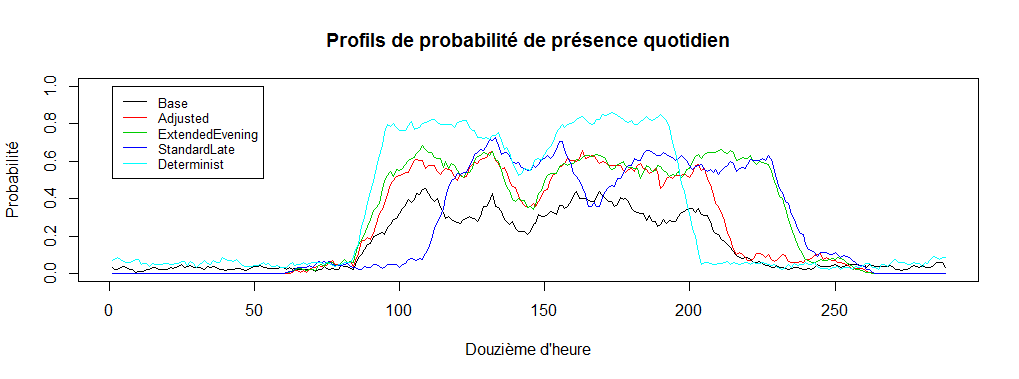
\includegraphics[scale=0.45]{Images/PageActivities/PresenceQ}
\caption{Profils de probabilité de présence quotidien moyens pour un agent simulé sur 1 année complète}
\label{fig:PresenceQ}
\end{figure}

\begin{figure}
\centering
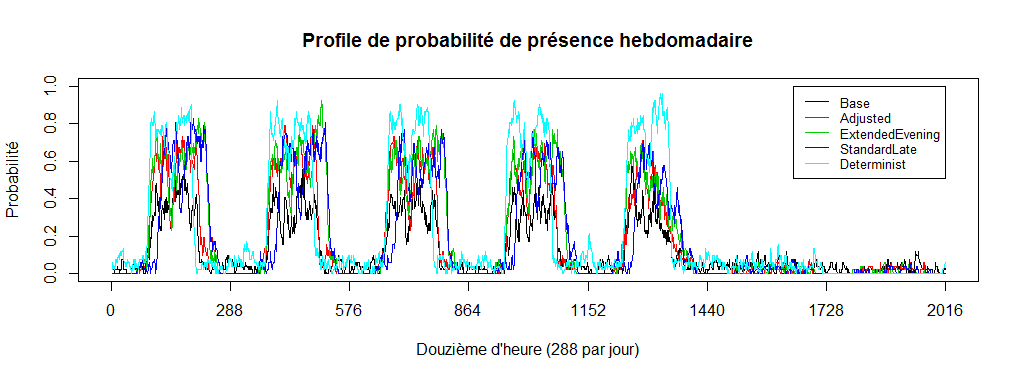
\includegraphics[scale=0.45]{Images/PageActivities/PresenceH}
\caption{Profils de probabilité de présence hebdomadaire moyens pour un agent simulé sur 1 année complète}
\label{fig:PresenceH}
\end{figure}

\begin{figure}
\centering
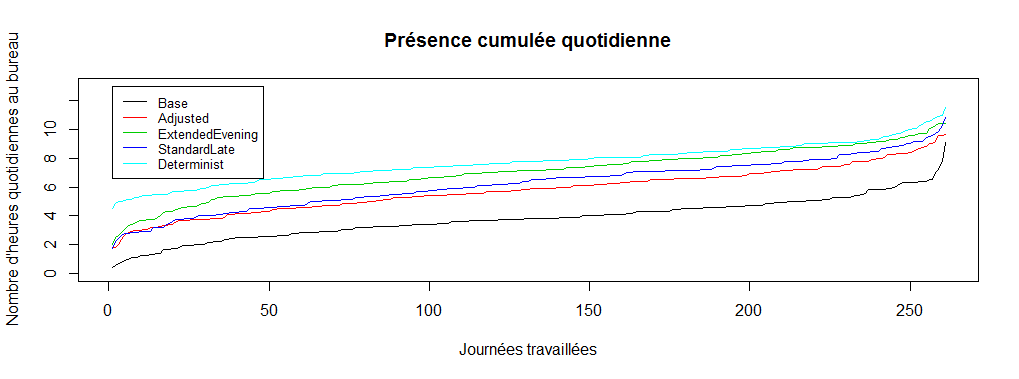
\includegraphics[scale=0.45]{Images/PageActivities/PresenceCumulee}
\caption{Distributions du nombre d'heures quotidiennes de présence pour un agent simulé sur 1 année complète}
\label{fig:PresenceCumulee}
\end{figure}

\begin{figure}
\centering
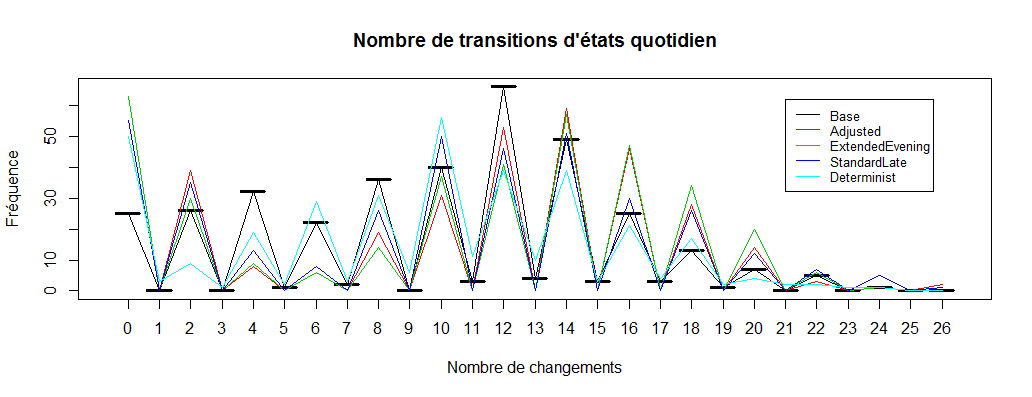
\includegraphics[scale=0.45]{Images/PageActivities/NbTransitions}
\caption{Distributions du nombre de transitions quotidien pour un agent simulé sur 1 année complète}
\label{fig:NbTransitions}
\end{figure}

\begin{figure}
\centering
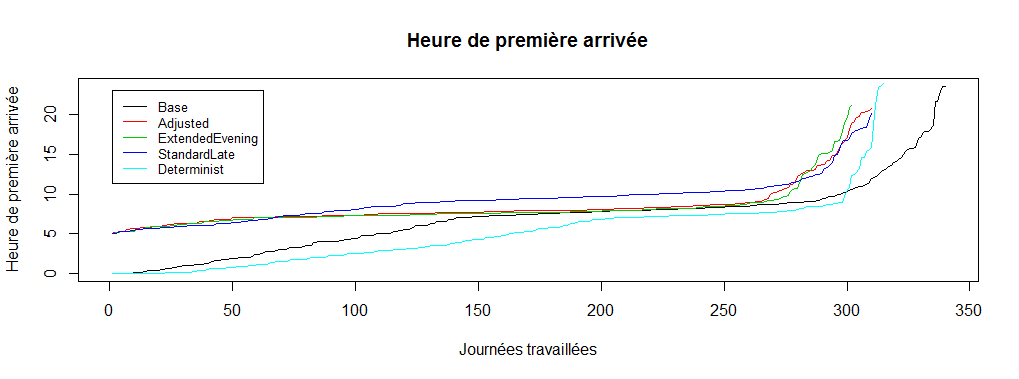
\includegraphics[scale=0.45]{Images/PageActivities/PremiereArrivee}
\caption{Distributions de l'heure de première arrivée dans le bureau pour un agent simulé sur 1 année complète}
\label{fig:PremiereArrivee}
\end{figure}

\begin{figure}
\centering
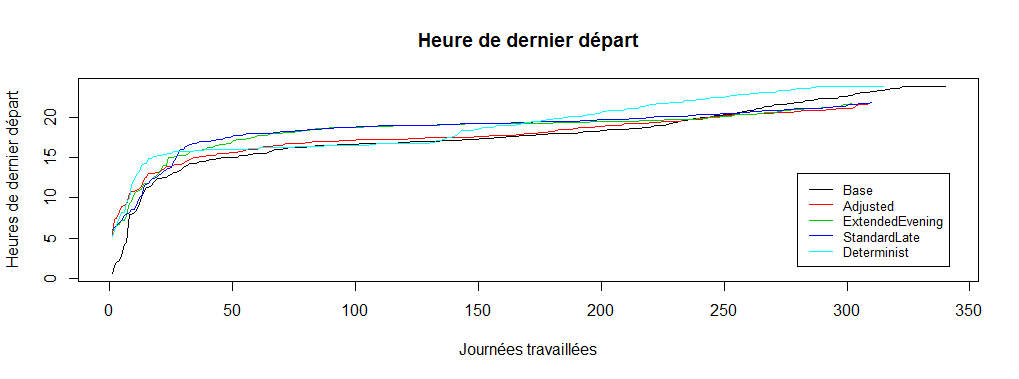
\includegraphics[scale=0.45]{Images/PageActivities/DernierDepart}
\caption{Distributions de l'heure de dernier départ dans le bureau pour un agent simulé sur 1 année complète}
\label{fig:DernierDepart}
\end{figure}

\newpage
\section{Activités dans les logements}
\label{ActivitésLogements}

Le fonctionnement général du modèle d'activités des logements est forcément très différent de celui des bureaux. Un point commun est qu'il est défini entièrement lors du pre-processus de la simulation. A la différence des bureaux, les activités dans les logements sont variées et ne sont donc pas limitées à la présence. Ces activités impliquent des comportements différents, des apports métaboliques différents dans les différentes zones du logement. La première partie de cette section présente l'état de l'art et plus particulièrement deux modèles qui nous ont interpellé et que nous avons opposé. La seconde partie porte sur la présentation détaillée du modèle de Jaboob \cite{Jaboob-16} répondant à nos exigences avec parcimonie. Le modèle idéal comporte un nombre de paramètres d'entrée limité, il rend compte de la diversité des activités en fonction du type d'habitants et produit des profils d'activités différents pour des individus semblables. Un modèle d'activités stochastique dans les logements convient alors parfaitement à la nature stochastiques des comportements humains.

\subsection{État de l'art}

L'état de l'art a permis de déterminer que l'ensemble des modèles d'activités proposés se base sur des enquêtes emploi du temps. Ces enquêtes se basent sur des échantillons de population larges (de l'ordre de 10000 participants) qui assurent une bonne représentativité des comportements de la vie quotidienne. Chaque répondant d'une enquête est associé à un descriptif socio-démographique et un carnet d'activités renseigné précisément sur une ou plusieurs journées. Le traitement de ces résultats permet de confronter les activités en cours avec les caractéristiques des individus. Ce traitement de données a mené à plusieurs modèles élaborés par Tanimoto et al. \cite{Tanimoto-08}, Widèn et al. \cite{Widen-12} ou encore Aerts et al. \cite{Aerts-14}, sans être exhaustif. Nous proposons dans la suite de détailler deux modèles qui ont particulièrement attirés notre attention, celui de Wilke et al. \cite{Wilke-13} et celui de Jaboob \cite{Jaboob-16}.

Vorger \cite{Vorger-14} reprend la stratégie de modélisation des activités dans les logements de Wilke et al. \cite{Wilke-13}. La base de données utilisée est issue de l'étude de 1998-1999\footnote{L'Enquête Emploi du Temps (EET) n'est plus disponible en ligne et a été remplacée par l'enquête plus récente de 2009-2010} de l'INSEE sur 7949 ménages et 15441 individus français qui ont noté leurs activités sur une journée toutes les 10 minutes. Le modèle proposé issu de cet EET permet dans une première étape de générer pour chaque occupant des périodes de présence et d'absence. Lorsqu'une période de présence débute, une des 20 activités débute également, suivant un modèle de Markov, et une durée lui est attribuée, suivant une loi de Weibull. Si l'activité prend fin avant la période d'absence alors une autre activité débute. En revanche, si une période d'absence commence avant la fin de l'activité alors cette dernière est abrogée. Les modèles de Markov et Weibull sont influencés par l'heure de la journée, par des caractéristiques du ménage et par des caractéristiques individuelles des occupants, rendant les profils d'activités très spécifique à chaque occupant. On peut néanmoins noter que ce modèle hybride présente quelques légers point d'amélioration à apporter. En effet, en raison de la non-continuité de l'enquête emploi du temps à minuit, les activités sont interrompus chaque jour à minuit conduisant à un début de période de sommeil quasi général à minuit et très rarement avant minuit. L'enquête datant de 1999, on peut également se demander si l'évolution des pratiques n'est pas suffisamment significative pour considérer une mise à jour. Aussi, le nombre de vingt activités renseignées nous semble excessif pour un exercice de modélisation de la performance énergétique.

Jaboob \cite{Jaboob-16} a plus récemment proposé un nouveau modèle d'activités basé sur une enquête emploi du temps anglaise datant de 2000-2001. La base de données est issue de questionnaires également renseignés toutes les 10 minutes sur une journée par 6500 ménages et 11700 individus. A partir de ces données, 10 modèles ont été développés et comparés. Il est conclu que le modèle de hybride Markov + Weibull fonctionne le mieux mais que le modèle de Bernoulli seul est recommandé pour sa simplicité et son faible nombre de paramètre d'entrées (240 contre 2880) tout en étant que très légèrement moins performant que le modèle hybride. Sur la base de ces conclusions, Chapman \cite{Chapman-16} utilise pour la prédiction des activités résidentiels ce modèle parcimonieux de Bernoulli, celui-ci ayant été recommandé. La qualité des modèles a été jugé en se basant sur 5 critères de validation et d'évaluation: 
\begin{itemize}
\item la sensibilité qui évalue la capacité du modèle à donner un résultat positif lorsqu'une hypothèse est vérifiée
\item la spécificité qui évalue la capacité du modèle à donner un résultat négatif lorsque l'hypothèse n'est pas vérifiée.
\item la précision qui regroupe la sensibilité et la spécificité
\item l'écart moyen à la moyenne, qui évalue l'amplitude de la différences de probabilité entre les simulations et les mesures.
\item l'indice de Brier, qui évalue la précision des probabilités du modèle
\end{itemize}

Or, nous notons qu'aucun de ces paramètres n'évalue le nombre de transitions d'état, qui nous semble pourtant fondamental pour reproduire des emplois du temps probables. Pour cette raison, il nous semble plus approprié d'utiliser un modèle d'activités hybride qui associe à chaque activité commencée une durée. Mahdavi et Tahmasebi \cite{Mahdavi-15} proposent un indicateur, sans unité, qu'ils appellent erreur du nombre de transitions et qui est défini par le nombre de transitions prédit moins le nombre de transitions mesurées. Ne possédant pas la base de donnée utilisée par Jaboob pour le développement du modèle, nous proposons dans la suite de simplement calculer le nombre de transitions d'état par jour issu des modèles et de les comparer.

\subsection{Processus de Bernoulli}

A partir de l'EET Anglaise, Jaboob \cite{Jaboob-16} propose un modèle permettant de générer 10 activités. En pré-processus, le modèle calcule pour chaque pas de temps l'activité réalisée pour les occupants. Le Tableau \ref{tab:Activités} les synthétise et associe à chaque activité le lieu où elles se produisent et l'état de l'occupant associé.

La diversité entre agents impacte leurs activités. Les variables explicatives des activités dans les logements sont relatives aux occupants (age, statut civique, genre, retraité/actif, chômeur/actif, niveau éducatif), au ménage (situation familiale, possession d'un ordinateur) et à l'environnement (heure de la journée, jour, saison). Le Tableau \ref{VariablesActivité} détaille ces variables et leurs différents niveaux.

\begin{table} [H]
\centering
\begin{tabular}{|p{5 cm}||p{5 cm}|p{5 cm}|}
\hline Activités & Localisation & État de l'occupant (Clo et Met [$W/m^{2}$]) \\
\hline
\hline 0- Dormir & Chambre & Clo = 2.55 \newline Met = 46 \\
\hline 1- Passif & Salon & Clo = 1 \newline Met = 58 \\
\hline 2- Audio-visuel & Salon & Clo = 1 \newline Met = 70 \\
\hline 3- Bureautique & Bureau ou chambre & Clo = 1 \newline Met = 116 \\
\hline 4- Cuisine & Cuisine & Clo = 1 \newline Met = 116 \\
\hline 5- Nettoyage & Cuisine & Clo = 1 \newline Met = 116 \\
\hline 6- Toilette corporelle & Salle de bain & Clo = 0 \newline Met = 116 \\
\hline 7- Vaisselle et machine à laver & Cuisine & Clo = 1 \newline Met = 93 \\
\hline 8- Bricolage & Salon & Clo = 1 \newline Met = 93 \\
\hline 9- Absent & Extérieur & .  \\
\hline
\end{tabular}
\normalsize
\caption{Nature des activités et états associés}
\label{tab:Activités}
\end{table}

\begin{table} [H]
\centering
\begin{tabular}{|p{4 cm}||p{11 cm}|}
\hline Variables & Niveaux - \textit{Codes} \\
\hline
\hline Age & Plus de 59 ans - \textit{age1} \newline Entre 36 et 59 and - \textit{age2} \newline Moins de 36 ans - \textit{age3} \\
\hline Statut civique & En couple (marié, concubinage, partenaire civique) - \textit{civstat1} \newline Célibataire - \textit{civstat2} \\
\hline Genre & Homme - \textit{sex1} \newline Femme - \textit{sex2} \\
\hline Retraité & Actif - \textit{retired0} \newline Retraité - \textit{retired1} \\
\hline Chômeur & Actif - \textit{unemp0} \newline Chômeur - \textit{unemp1} \\
\hline Éducation & Lycée ou moins - \textit{edtry1} \newline Premier cycle - \textit{edtry2} \newline Second cycle et plus - \textit{edtry3}  \\
\hline Situation familiale & Adulte(s) sans enfants - \textit{famstat0} \newline Adulte(s) avec bébé (moins de 5 ans) - \textit{famstat1} \newline Adulte(s) avec enfants (entre 5 et 18 ans) - \textit{famstat2} \newline Adulte de plus de 40 ans sans enfants - \textit{famstat3} \newline Enfant avec parents ou garde - \textit{famstat4} \newline Enfant sans parents ou garde - \textit{famstat5} \\
\hline Possession d'ordinateur & Non - \textit{computer0} \newline Oui - \textit{conputer1} \\
\hline Heure & \textit{1 - 24} \\
\hline Jour & Lundi : Dimanche - \textit{day1} : \textit{day7} \\
\hline Saison & Printemps - \textit{season1} \newline Eté - \textit{season2} \newline Automne - \textit{season3} \newline Hiver - \textit{season4} \\
\hline
\end{tabular}
\normalsize
\caption{Variables sélectionnées pour expliquer les activités des occupants}
\label{VariablesActivité}
\end{table}

L'équation ci-dessous, issue de la régression logistique multinomial de l'EET, permet de calculer la probabilité, $P_{j}(x,t)$ de commencer une nouvelle activité.

\begin{equation}
P_{j}(x,t)=\frac{exp(A_{j}(x))}{\sum\limits_{j=1}^{N}exp(A_{j}(x))}, j = 1, .., N et A_{j}(x)= \alpha_{j}+\sum\limits_{k=1}^{n}\beta_{jk}x_{jk}
\end{equation}

N correspond au nombre d'activités total, soit 10, n correspond au nombre de prédicteurs, soit 10 (nombre de variables dans le Tableau \ref{VariablesActivité} excepté l'heure), $\alpha$ et $\beta$ sont respectivement l'interception et la pente. Les probabilités de commencer une activité dépendent ainsi des caractéristiques des occupants mais également du temps, en émane donc pour chaque occupant une matrice à 4 dimensions [10][24][7][4] (activités, heures, jour de la semaine et saison, respectivement).

\subsection{Modèle hybride}

Le modèle hybride couple au modèle de Bernoulli un modèle de Weibull. Ainsi, lorsqu'une activité débute, une durée correspondante y est associée. Wilke propose dans son modèle d'activités des coefficients de durée désagrégés. Bien sûr, les fonctions de Weibull diffèrent temporellement, la durée de l'activité de sommeil est plus longue si elle commence en début de nuit qu'en début d'après-midi, mais elle diffèrent également selon les caractéristiques des occupants, la durée d'un repas pour un retraité est plus longue que pour un actif. Pour considérer ces caractéristiques liées aux occupants les données sont structurées en arbres binaires. Pour chaque activité et chaque heure de la journée un arbre binaire est proposé, les nœuds de celui-ci étant formé par les attributs des occupants.

Au contraire, Jaboob \cite{Jaboob-16} fourni dans sa thèse les coefficients de forme et d'échelle de manière agrégés pour chaque heure et activité de la simulation, mais pas en fonction des caractéristiques des occupants. L'auteur justifie ce choix par un modèle davantage parcimonieux et une plus-value discutable de la désagrégation, les distinctions étant très peu intuitives et les caractéristiques des individus  multi-colinéaires. Pour ces raisons, nous décidons d'utiliser les coefficients agrégés de Jaboob.

La durée de l'équation est alors définie par l'équation ci-dessous, U étant un nombre aléatoire tiré entre 0 et 1. 

\begin{equation}
t_{j}=\frac{(-log(U))^{\frac{1}{k}}}{\lambda}
\end{equation}

Les paramètres de forme $k$ et d'échelle $\lambda$, déterminés par la méthode du maximum de vraisemblance, maximisent la probabilité de reproduire, par une loi de Weibull, la distribution observée de l'enquête emploi du temps.

Il est à noter que les coefficients de la loi de Weibull ne sont pas connus pour l'activité informatique (\textit{IT}) lorsqu'elle a lieu de 2 à 4 heures du matin dans la base de donnés de Jaboob. Cela est la conséquence d'un événement peu ou pas présent à ces heures dans la base de données. Pour s'affranchir de cette méconnaissance problématique pour le modèle, nous proposons une simple interpolation linéaire basée sur les intervalles de temps précédent et suivant:
\begin{equation}
f(x)=\frac{x_{b}-x}{x_{b}-x_{a}}y_{a}+\frac{x-x_{a}}{x_{b}-x_{a}}y_{b}
\end{equation}
Sachant que $\lambda(2)=61.806$ et que $\lambda(5)=40.125$ on a alors $\lambda(3)=54.579$ et $\lambda(4)=47.352$. Et sachant que $k(2)=1.143$ et que $k(5)=0.813$ on a alors $k(3)=1.033$ et $k(4)=0.923$. L'ensemble des coefficients se trouve en Annexe de la thèse de Jaboob \cite{Jaboob-16}.

\subsection{Présentation des résultats}

Afin de tester et visualiser les sorties des modèles d'activités dans les logements, nous avons généré un ensemble de graphiques, Figure \ref{fig:Activités}, qui présente les profils d'activités journaliers de 2 occupants différents, le premier est un jeune homme de 20 ans, avec ordinateur, actif et célibataire alors que le second est un retraité marié de 60 ans, sans ordinateur, sous les deux types de modèles, Bernoulli et hybride. Les profils générés par les deux familles de modèle sont globalement en accord avec le sens commun, nous pouvons néanmoins émettre un certain nombre de critiques. Pour la comparaison d'archétype, on retrouve sans surprise une proportion de temps à l'extérieur très supérieur chez l'occupant actif que chez le retraité, une durée devant la télévision supérieure pour le retraité ou encore une période de sieste plus significative chez les retraités. Étonnamment, plusieurs activités sont réparties uniformément sur la période d'éveil, comme l'activité cuisine dont on attendait des pics aux heures de repas. Également étonnamment, on note une importante proportion de l'activité informatique à 9 et 14 heure chez l'occupant retraité. Pour la comparaison des deux modèles on a tendance à penser que le modèle hybride reproduit mieux le sommeil que le modèle de Bernoulli qui génère assez peu d'heures de sommeil et un nombre d'autres activités semble t-il élevé. L'activité douche-toilette se retrouve dans le modèle hybride quant à elle réduite mais les deux pics du matin et du soir restent visibles.

La Figure \ref{fig:ExempleScenario} permet d'évaluer le nombre de transitions entre deux activités. Sans surprise, nous ne notons pas de différences significatives entre le nombre de transitions entre deux catégories d'occupants, au contraire du type de modèle. Sur 150 jours de simulations, le modèle de Bernoulli a généré en moyenne 185 activités quotidienne contre 56 pour le modèle hybride, pour un pas de temps de 5 minutes. Cet indicateur est difficile à interpréter rigoureusement car nous n'avons pas identifié de valeur étalonnée dans la littérature. En effet, l'enquête emploi du temps est à pas de temps fixe, plusieurs activités peuvent alors avoir lieu sur un même pas de temps sans être prise en compte dans l'enquête. Le nombre d'activités recensés dans l'enquête est également de grande influence sur le nombre de changement d'états. Enfin, le pas de temps de simulation, impacte considérablement ce nombre de transitions. Une simulation au pas de temps de 10 minutes a mené à 14 transitions, contre les 56 au pas de 5 minutes. Cet indicateur de nombre de transitions n'est en revanche pas sans intérêt, d'une part car il peut être utilisé pour comparer des modèles, ici le modèle de Bernoulli seul au modèle hybride Bernoulli (pour déterminer le début des activités) + Weibull (pour déterminer les durées des activités) et d'autres part pour mieux appréhender la dynamique des occupants dans ce modèle de prédiction des activités.

Comme nous l'avons indiqué en introduction, nous ne proposons pas pour le modèle d'activités dans les logements résidentiels d'adaptation contextuelle supplémentaire, car le modèle initial comporte de base 11 variables. Nous estimons donc que le développement de ce modèle a suffisamment bien intégré la diversité d'activité des occupants sans devoir à l'accentuer. 

\begin{figure}[H]
\centering
\begin{tabular}{cc}
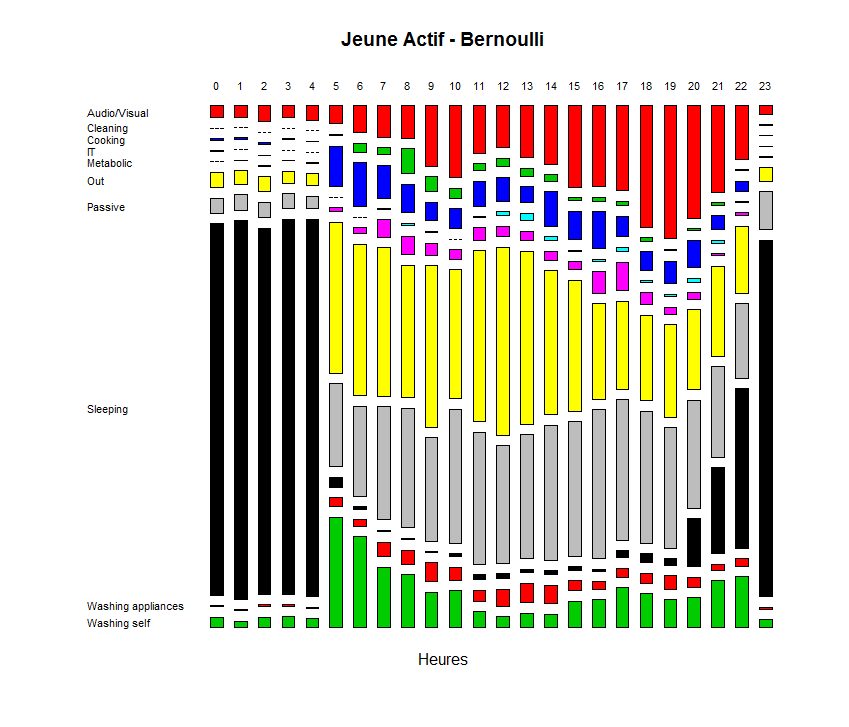
\includegraphics[scale=0.38]{Images/Activites/JeuneActifBernoulli} &
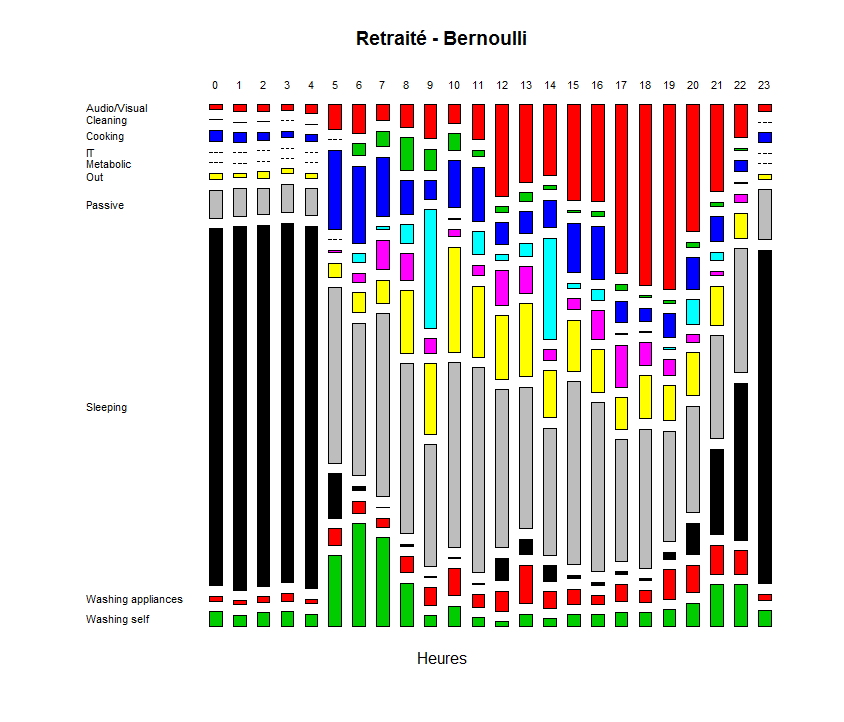
\includegraphics[scale=0.38]{Images/Activites/RetraiteBernoulli} \\
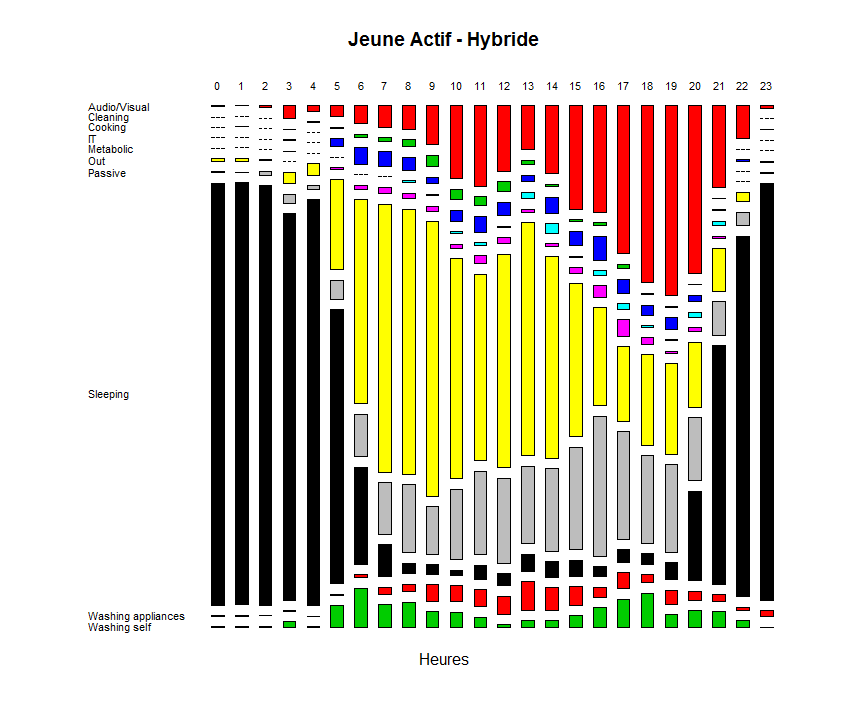
\includegraphics[scale=0.38]{Images/Activites/JeuneActifHybride} &
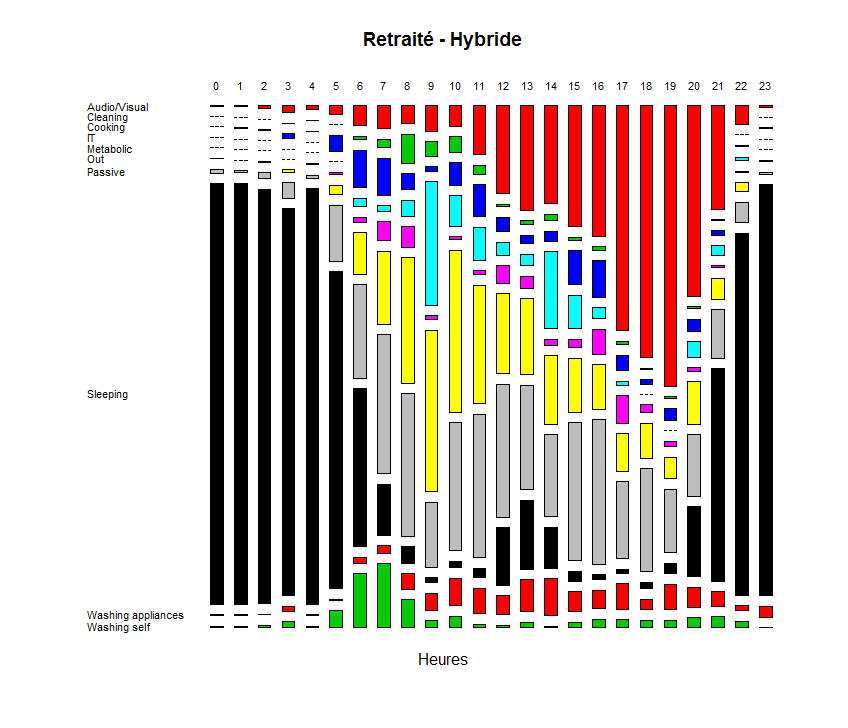
\includegraphics[scale=0.38]{Images/Activites/RetraiteHybride} \\
\end{tabular}
\caption{Chronogramme moyen des activités sur une journée calculé sur 150 jours, pour un jeune actif (à gauche) et pour un retraité (à droite), selon le modèle de Bernoulli (en haut) et le modèle hybride Bernoulli + Weibull(en bas), toutes choses égales par ailleurs}
\label{fig:Activités}
\end{figure}

\begin{figure}[H]
\centering
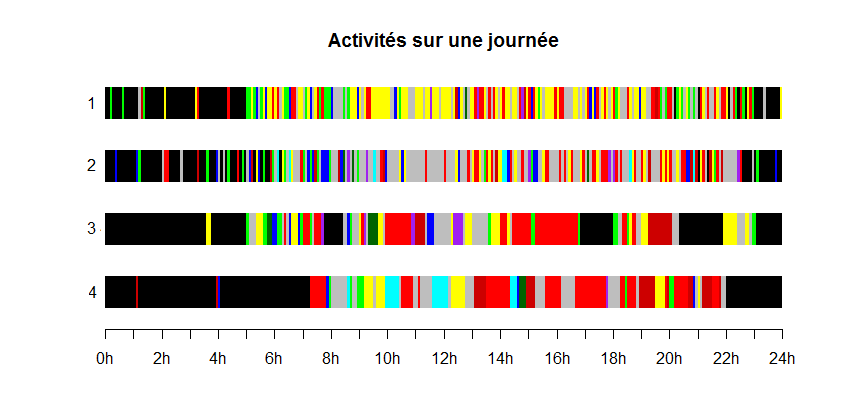
\includegraphics[scale=0.7]{Images/Activites/ActivitesSurUneJournee}
\caption{Exemple de scénarios d'activités pour une journée d'hiver pour; 1- l'actif avec le modèle de Bernoulli, 2- le retraité avec le modèle de Bernoulli, 3- l'actif avec le modèle hybride, 4- le retraité avec le modèle hybride. Le code couleur est le même que pour la Figure \ref{fig:Activités}}
\label{fig:ExempleScenario}
\end{figure}

\part{Application et perspectives}

\chapter{Analyse de sensibilité sur bâtiment résidentiel}

\section{Présentation de l'opération}

Les Terrasses d'Iberville...

\section{•}
\chapter{Discussion}

\section{La problématisation avant la modélisation}

Avant de modéliser un phénomène il faut le problématiser. Cela renvoi à des démarches intellectuelles différentes et d'orientation opposées. Aujourd'hui la modélisation est l'approche communément utilisée par les ingénieurs et la problématisation est plutôt utilisée en sciences humaines et sociales.

2009 - Michelot Christian - Modélisation ou problématisation?

\section{Appropriation de la technologie}

Suite à l'apparition des préoccupations environnementales, les bâtiments sont de plus en plus performants, mais aussi de plus en plus standardisés, car soumis à des réglementations toujours plus exigeantes. Pour répondre à ces exigences, les acteurs du bâtiment n'ont pas eu d'autres choix que d'y intégrer les nouvelles technologies et les habitants n'ont pas eu le choix de les assimiler. Or d'après Beslay \cite{Beslay-08}, s'approprier, c'est transformer. En effet, les bâtiments récents sont exigent en terme d'usage et impliquent de nouvelles habitudes, tout en étant devenus difficiles à régler, à exploiter et à habiter. Cette difficulté d'utilisation des bâtiments performants, résulte alors parfois en des comportements déviant voir absurdes qu'il faut corriger pour atteindre les objectifs environnementaux mais également de confort.

\section{L'accompagnement des usagers}

Modéliser le comportement des usagers des bâtiments, ne va pas résoudre seul le problème de performances énergétiques décevantes. Cela va permettre de mieux comprendre les usages et de mieux les appréhender lors du processus de conception ou rénovation des bâtiments. Cette nouvelle connaissance doit en retour profiter aux occupants, par leur accompagnement. Cet activité, généralement sous le nom d'Assistance à Maitrise d'Usage, est en plein essor. 

En région Rhône-Alpes, Vie to B\footnote{Site officiel de Vie to B: \url{http://vie-to-b.fr/}, visité le 23/02/2016} est spécialisé dans l'accompagnement de l'usage de bâtiments performants. Ils ont pour missions principales d'accompagner les occupants dans l'appropriation de leur logement et de les accompagner dans la conciliation entre confort et performance énergétique.

Brisepierre et al. \cite{Brisepierre-15}, dans l'ouvrage "l'accompagnement des occupants: Une évidence à déconstruire", démontrent tout l'intérêt  ...

Lenormand et al. \cite{Lenormand-15}, lors des Journées Internationales de la Sociologie de l'Energie, ont remis en cause les pratiques des énergéticiens qu'ils jugent décorélées des usages quotidiens.


\section{Conclusion}

Nous avons vu dans les chapitres précédents que la sociologie est une science qui permet d'aider au développement de modèles physiques, d'une part dans l'élaboration de questionnaires, d'interviews ou de suivi de mesures mais également dans le traitement des résultats et de l'interprétation qui peut en être faite.

Ce chapitre démontre également que la seule modélisation ne peut pas résoudre les défaillances d'usages, mais qu'un accompagnement personnalisé des usagers est en revanche une solution fiable et durable à mettre en avant dans les prochaines opérations neuves ou de rénovations.

\bibliographystyle{ieeetr}
\bibliography{mabiblio}

\end{document}


